% !TeX program = lualatex
% !TeX spellcheck = en_US
% !TeX encoding = UTF-8

%https://www.forrestthewoods.com/blog/memory-bandwidth-napkin-math/

% COMPILE WITH:
% latexmk -pdflatex=lualatex -pdf -outdir=build %
% You need lualatex and biber (in all TeXLive distributions)
\documentclass{beamer}
\usepackage{fontawesome} %using symbols
\usepackage{ifthen} %conditional commands
\usepackage{xstring} %for string comparisons
\usepackage{adjustbox}
\usepackage{tabularx}
\usepackage{tikz}
\usepackage{ulem}
\usepackage[american]{babel} %ngerman
\usepackage{graphicx}
\usepackage{pgf}
\usepackage{layouts} %DEBUG
%\usepackage{svg}
\usepackage{amsmath}
\usepackage{unicode-math}   % lädt auch fontspec!
\usepackage{mathtools}
%usepackage{polyglossia}
%\setdefaultlanguage[variant=american]{english}
%\setmainlanguage{german}
%\usepackage{luacode}
\usepackage{csquotes}
\usepackage{cancel}
\usepackage{url}
\usepackage{multirow}

%\usepackage{enumerate}
%\usepackage[nowarn,acronym]{glossaries}
\usepackage[nolist,nohyperlinks]{acronym}
\usepackage{verbatim}
\usepackage{pdfpages}

%\usepackage{tikz}
\usepackage{caption}
\usepackage{subcaption}
\usepackage{wrapfig} %NEEDS height or might break page
\usepackage{tcolorbox}
\usepackage{adjustbox}
%\usepackage{wraptable} %DOES NOT EXIST
%\usepackage{showframe} %DEBUG LAYOUT
%\usepackage{pgfplots}	%USE PGF
%\usepgfplotslibrary{external} %external BROKEN
\usepackage[linesnumbered,ruled,vlined]{algorithm2e}
%\usepackage[plainpages=false]{hyperref} %doesnt work in beamer
%\usepackage{algorithm}
%\usepackage{algpseudocode}
\usepackage[backend=biber]{biblatex}

\begin{acronym}
  \acro{srg}[SRG]{Seeded Region Growing}
  \acro{ccl}[CCL]{Connected Components Labeling}
  \acro{simpa}[\texttt{simpaSRG}]{\texttt{simple parallel Seeded Region Growing}}
  \acro{rbrg}[RBRG]{Raster Based Region Growing}
  \acro{sbrg}[SBRG]{Superpixel-based Region Growing}
  \acro{mad}[MAD]{Memory access delay}
  \acro{ns}[ns]{nanoseconds}
\end{acronym}

\bibliography{references.bib}

%https://tex.stackexchange.com/questions/285578/how-to-draw-parallelepiped-and-cube-with-latex/288101#288101
%for loops https://tex.stackexchange.com/questions/29877/need-help-creating-a-3d-cube-from-a-2d-set-of-nodes-in-tikz
\newcommand{\tikzcuboid}[4]{% width, height, depth, scale
\begin{tikzpicture}[scale=#4]
\foreach \x in {0,...,#1}
{   \draw (\x ,0  ,#3 ) -- (\x ,#2 ,#3 );
    \draw (\x ,#2 ,#3 ) -- (\x ,#2 ,0  );
}
\foreach \x in {0,...,#2}
{   \draw (#1 ,\x ,#3 ) -- (#1 ,\x ,0  );
    \draw (0  ,\x ,#3 ) -- (#1 ,\x ,#3 );
}
\foreach \x in {0,...,#3}
{   \draw (#1 ,0  ,\x ) -- (#1 ,#2 ,\x );
    \draw (0  ,#2 ,\x ) -- (#1 ,#2 ,\x );
}
\end{tikzpicture}
}
\newcommand{\tikzcube}[2]{% length, scale
\tikzcuboid{#1}{#1}{#1}{#2}
}
\newcommand{\floor}[1]{\lfloor #1 \rfloor}
\captionsetup[figure]{font=small}
\captionsetup[subfigure]{singlelinecheck=off,justification=raggedright,font=scriptsize}
%\captionsetup{singlelinecheck=off,justification=raggedleft,labelformat=empty,labelsep=none}

\title{Robust, in-place, parallelized Seeded Region Growing for 3D image segmentation}
\subtitle{
  Studienarbeit \textsl{Medizin}
}
  %\\[1ex]
  %\insertdate\\[1ex]
  %\insertauthor\\[1ex]
\author{Jan Philipp Hafer\\[1ex]
Supervisor Dr. Felix Gremse}
\date{Winter Semester 2020}

\begin{document}
\begin{frame}[plain]
  \titlepage
\end{frame}
\begin{frame}{Table of Contents}
  \tableofcontents
\end{frame}
\section{Algorithm input - shapes of 3D scan data}
\begin{frame}{\insertsection}
\begin{minipage}{0.5\textwidth}%
  Voxel (size 1 Byte):
\tikzcuboid{1}{1}{1}{0.5}\\
  Cube ($4\times 4\times 4=64$B):
\tikzcuboid{4}{4}{4}{0.5}\\
  Cuboid:\\
\tikzcuboid{8}{4}{4}{0.5}
\end{minipage}%
\begin{minipage}{0.5\textwidth}%
  Path: \tikzcuboid{4}{1}{1}{0.5}\\
  Dilation: \tikzcuboid{2}{2}{2}{0.5}\\
  Dilated path: \tikzcuboid{5}{2}{2}{0.5}
\end{minipage}%
\end{frame}
\section{Seeded Region Growing}
\begin{frame}
  \tableofcontents[currentsection]
\end{frame}
\subsection{Why Seeded Region Growing?}
\begin{frame}{Why~\ac{srg}?}
  Purpose of~\ac{srg}:\\
  Determine and visualize connected voxel of a 3D scan for patient treatment from a user-defined starting point.\\
  %voxel do not need to be cubic!
  \vspace{1cm}
  \begin{enumerate}
      \item simple
      \item fast
      \item robust
  \end{enumerate}
\end{frame}

\begin{frame}{\Ac{srg} in 2D}
\centering
\begin{tcolorbox}[boxsep=1pt,left=0pt,right=0pt,top=0pt,bottom=0pt,title=round 0]
\begin{figure}[h]
\begin{subfigure}[b]{0.15\linewidth}%
\centering
  \includegraphics[width=0.8\linewidth]{figures/srg1.pdf}
  %\\queue:\cancel{(1,1)}}
\end{subfigure}%a)
\end{figure}
\end{tcolorbox}
\begin{tcolorbox}[boxsep=1pt,left=0pt,right=0pt,top=0pt,bottom=0pt,title=round 1]
\begin{figure}[h]
\begin{subfigure}[b]{0.15\linewidth}%
\centering
  \includegraphics[width=0.8\linewidth]{figures/srg2.pdf}
  %\\queue:}
\end{subfigure}%b)
\begin{subfigure}[b]{0.15\linewidth}%
\centering
  \includegraphics[width=0.8\linewidth]{figures/srg3.pdf}
  %\\queue:}
\end{subfigure}%c)
\begin{subfigure}[b]{0.15\linewidth}%
\centering
  \includegraphics[width=0.8\linewidth]{figures/srg4.pdf}
  %\\queue:(2,3)}
\end{subfigure}%d)
\begin{subfigure}[b]{0.15\linewidth}%
\centering
  \includegraphics[width=0.8\linewidth]{figures/srg5.pdf}
  %\\queue:(2,3),(3,2)}
\end{subfigure}%e)
\end{figure}
\end{tcolorbox}
\begin{tcolorbox}[boxsep=1pt,left=0pt,right=0pt,top=0pt,bottom=0pt,title=round 2]
\begin{figure}[h]
\begin{subfigure}[b]{0.15\linewidth}%
\centering
  \includegraphics[width=0.8\linewidth]{figures/srg6.pdf}
  %\\queue:\cancel{(2,3)},(3,2)}
\end{subfigure}%f)
\begin{subfigure}[b]{0.15\linewidth}%
\centering
  \includegraphics[width=0.8\linewidth]{figures/srg7.pdf}
  %\\queue:(3,2)}
\end{subfigure}%g)
\begin{subfigure}[b]{0.15\linewidth}%
\centering
  \includegraphics[width=0.8\linewidth]{figures/srg8.pdf}
  %\\queue:(3,2)}
\end{subfigure}%h)
\begin{subfigure}[b]{0.15\linewidth}%
\centering
  \includegraphics[width=0.8\linewidth]{figures/srg9.pdf}
  %\\queue:(3,2),(3,3)}
\end{subfigure}%i)
\begin{subfigure}[b]{0.15\linewidth}%
\centering
  \includegraphics[width=0.8\linewidth]{figures/srg10.pdf}
  %\\queue:\cancel{(3,2)},(3,3)}
\end{subfigure}%j)
\begin{subfigure}[b]{0.15\linewidth}%
\centering
  \includegraphics[width=0.8\linewidth]{figures/srg11.pdf}
  %\\queue:(3,3)}
\end{subfigure}%k)
\end{figure}
\end{tcolorbox}
\begin{tcolorbox}[boxsep=1pt,left=0pt,right=0pt,top=0pt,bottom=0pt,title=round 3]
\begin{figure}
\begin{subfigure}[b]{0.15\linewidth}%
\centering
  \includegraphics[width=0.8\linewidth]{figures/srg12.pdf}
  %\\queue:\cancel{(3,3)}}
\end{subfigure}%l)
\begin{subfigure}[b]{0.15\linewidth}%
\centering
  \includegraphics[width=0.8\linewidth]{figures/srg13.pdf}
  %\\queue:}
\end{subfigure}%m)
\begin{subfigure}[b]{0.15\linewidth}%
\centering
  \includegraphics[width=0.8\linewidth]{figures/srg14.pdf}
  %\\queue:}
\end{subfigure}%n)
\end{figure}
\end{tcolorbox}
\end{frame}

\subsection{\Ac{srg} in 3D}
\begin{frame}{\insertsubsection : round 1}
  %\centering \vspace{-0.55cm}
  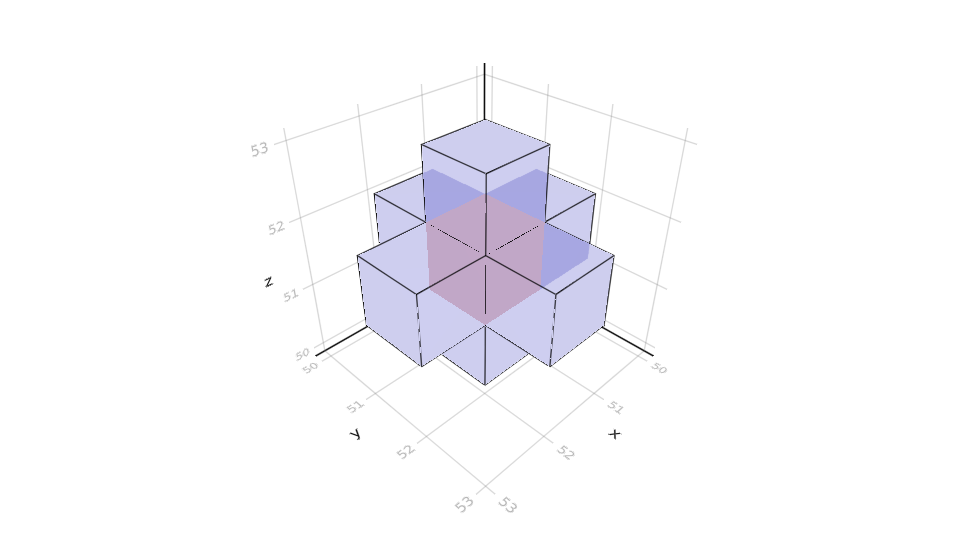
\includegraphics[trim=5cm 0.7cm 5cm 3cm, clip, width=1\linewidth]{algorithm_visualisation/srgsteps/srgstep0.png}\\
  \rightline{\color{gray} theory}
\end{frame}
\begin{frame}{\insertsubsection : round 2}
  %\centering \vspace{-0.55cm}
  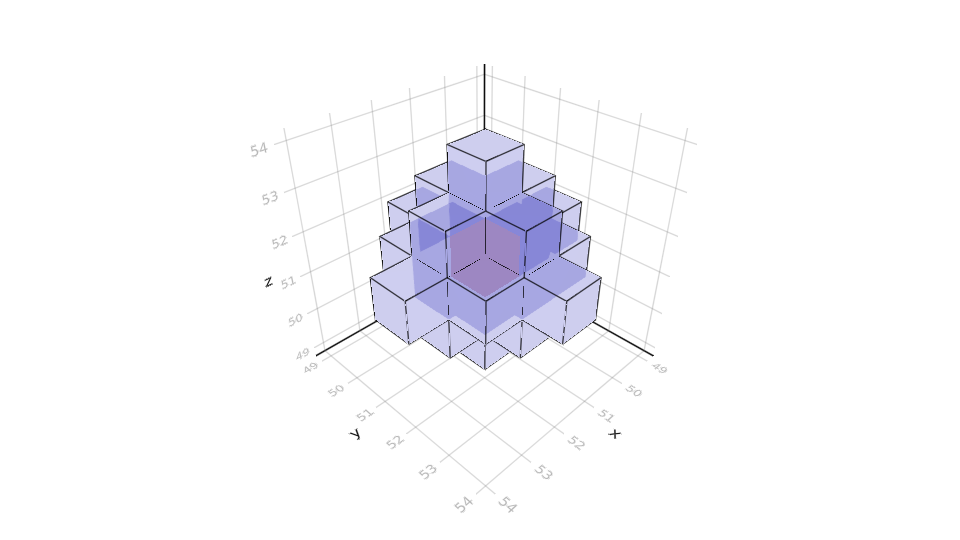
\includegraphics[trim=5cm 0.7cm 5cm 3cm, clip, width=1\linewidth]{algorithm_visualisation/srgsteps/srgstep1.png}\\
  \rightline{\color{gray} theory}
\end{frame}
\begin{frame}{\insertsubsection : round 3}
  %\centering \vspace{-0.55cm}
  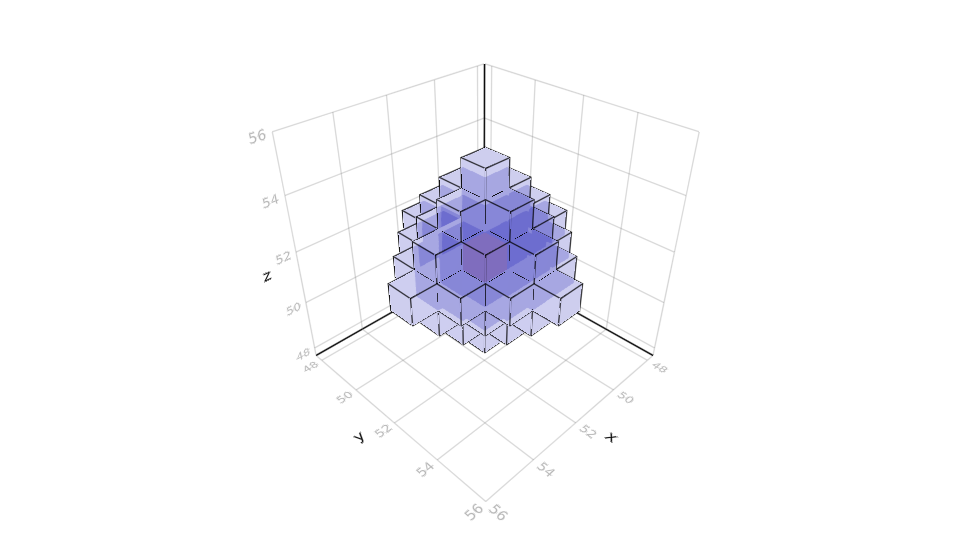
\includegraphics[trim=5cm 0.7cm 5cm 3cm, clip, width=1\linewidth]{algorithm_visualisation/srgsteps/srgstep2.png}\\
  \rightline{\color{gray} theory}
\end{frame}
\begin{frame}{\insertsubsection : round 4}
  %\centering \vspace{-0.55cm}
  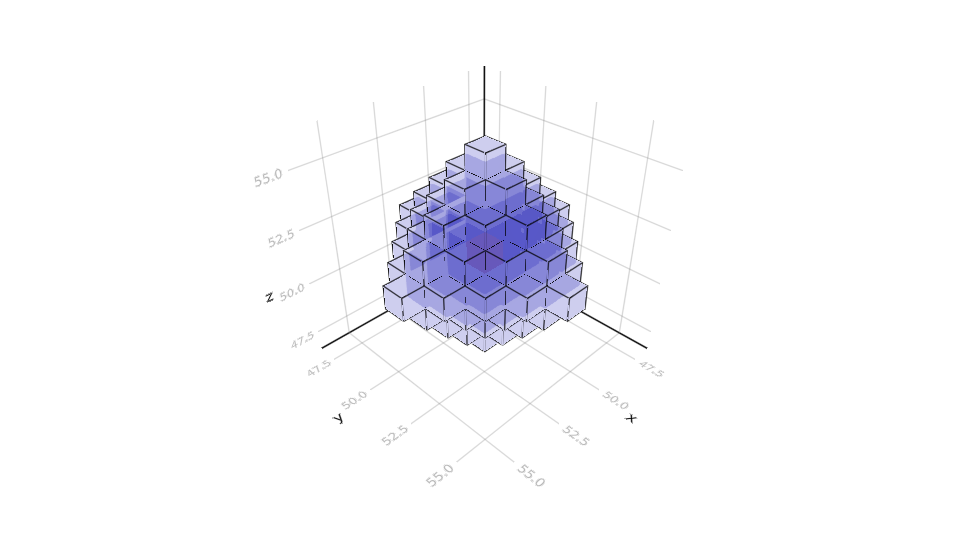
\includegraphics[trim=5cm 0.7cm 5cm 3cm, clip, width=1\linewidth]{algorithm_visualisation/srgsteps/srgstep3.png}\\
  \rightline{\color{gray} theory}
\end{frame}
\begin{frame}{\insertsubsection : round 5}
  %\centering \vspace{-0.55cm}
  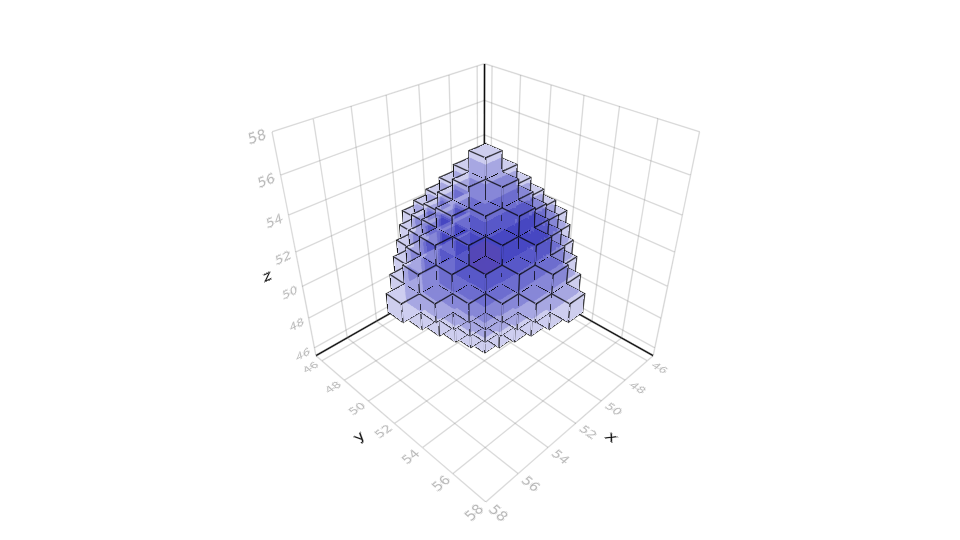
\includegraphics[trim=5cm 0.7cm 5cm 3cm, clip, width=1\linewidth]{algorithm_visualisation/srgsteps/srgstep4.png}\\
  \rightline{\color{gray} theory}
\end{frame}
\begin{frame}{\insertsubsection : round 6}
  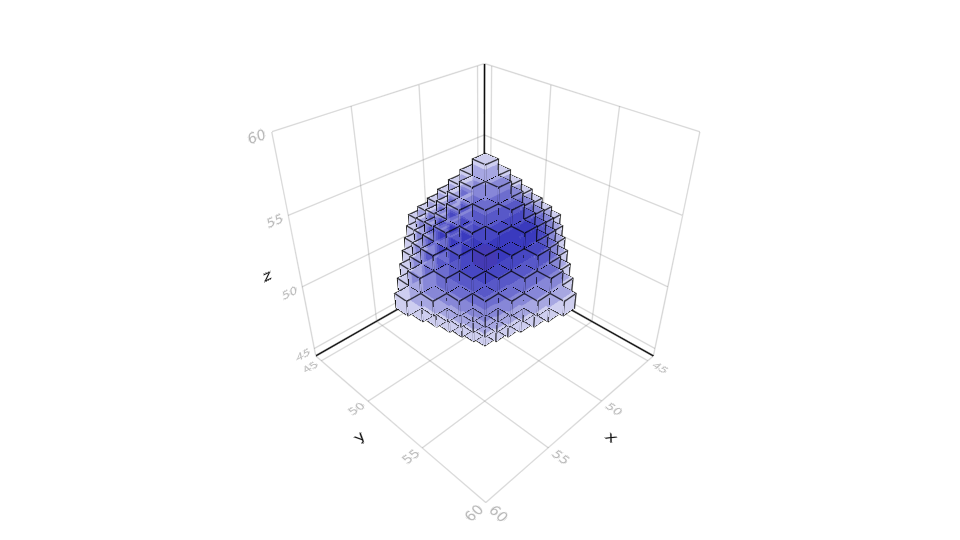
\includegraphics[trim=5cm 0.7cm 5cm 3cm, clip, width=1\linewidth]{algorithm_visualisation/srgsteps/srgstep5.png}\\
  \rightline{\color{gray} theory}
\end{frame}
\begin{frame}{\insertsubsection : round 7}
  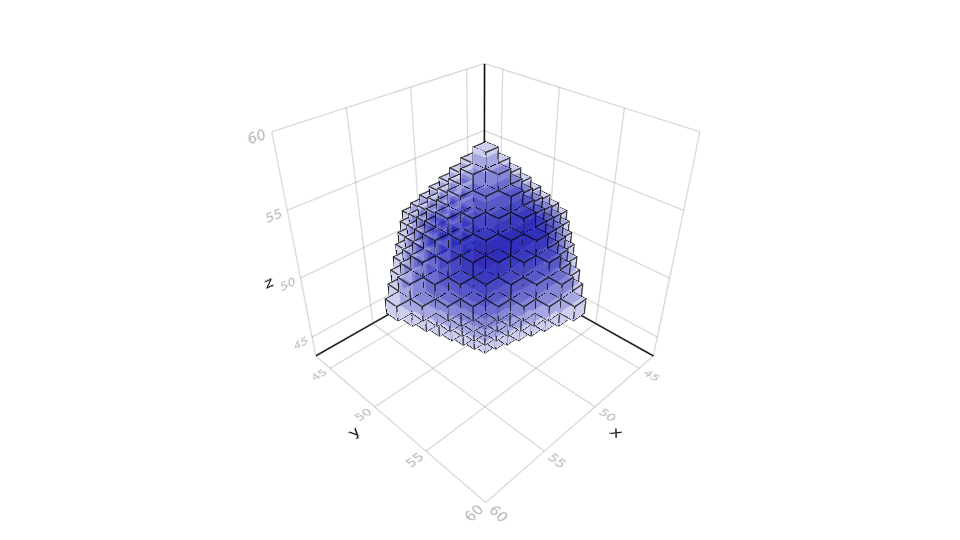
\includegraphics[trim=5cm 0.7cm 5cm 3cm, clip, width=1\linewidth]{algorithm_visualisation/srgsteps/srgstep6.png}\\
  \rightline{\color{gray} theory}
\end{frame}
\begin{frame}{\insertsubsection : round 11}
  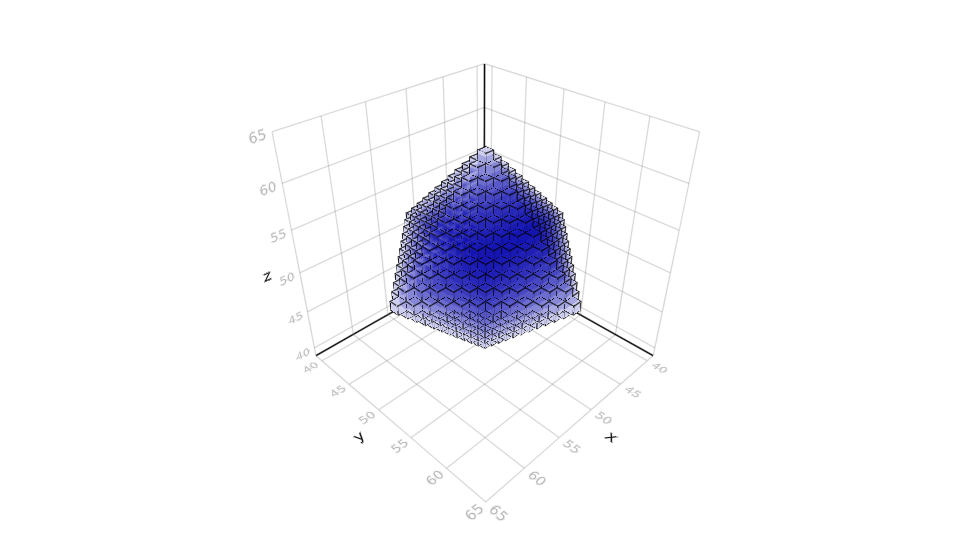
\includegraphics[trim=5cm 0.7cm 5cm 3cm, clip, width=1\linewidth]{algorithm_visualisation/srgsteps/srgstep10.png}\\
  \rightline{\color{gray} theory}
\end{frame}
\begin{frame}{\insertsubsection : round 46}
  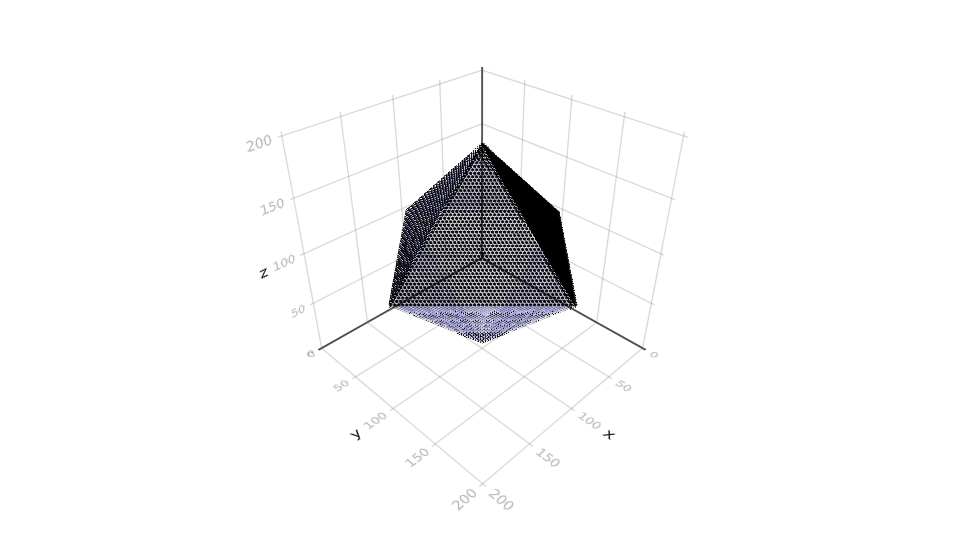
\includegraphics[trim=5cm 0.7cm 5cm 3cm, clip, width=1\linewidth]{algorithm_visualisation/srgsteps/srgstep45.png}\\
  octahedron - dual object to cube\\
  \rightline{\color{gray} theory}
\end{frame}
%\SetAlCapNameFnt{\scriptsize}
%\SetAlCapFnt{\scriptsize}
%\begin{algorithm}[H]
%  \DontPrintSemicolon
%  %\algsetup{linenosize=\scriptsize}
% \scriptsize
%  \caption{\Ac{srg} by Adams and Bischoff} \label{alg:srg}
%  \KwData{Vector \texttt{data} as voxels with values 0(invalid) or 1(valid)}
%  \KwResult{Vector \texttt{data} as voxels with values 0(invalid), 1(unmarked) and 255(marked)}
%  queue.push(seeding\_point); \tcp*{$(x,y,z)$} 
%  \While{queue.empty() == false}{
%    first\_element =  queue.front(); \tcp*{$(x,y,z)$}
%    queue.pop();\\
%    \ForAll{neighbors of first\_element}{
%      \tcc*{neighbor $\in \{(x\pm 1,y,z),(x,y\pm 1,z),(x,y,z\pm 1)\}$}
%      \If {neighbor $\in \text{Cuboid}(x_\text{max},y_\text{max},z_\text{max})$} {
%        %\tcc*{neighbor $(x,y,z)$ is in Cuboid-shaped input data}
%        offset $= x_\text{max}*y_\text{max}*z+x_\text{max}*y+x$;\\
%        neighborValue = \texttt{data}[offset];\\
%        \If{neighborValue == 1}{
%          neighborValue = 255;\\
%          queue.push(neighbor);
%        }
%      }
%    }
% }
%\end{algorithm}
\subsection{Memory access delay}
\begin{frame}{\insertsubsection}
  \centering
  \ac{mad}: Time delay of accessing data for modification in CPU core
  \begin{table}
    \small
    \caption{Memory types with~\ac{mad} on Intel x86\_64 as of 2020\footnote{\url{https://stackoverflow.com/questions/4087280/approximate-cost-to-access-various-caches-and-main-memory/33065382\#33065382}}}
    \begin{tabularx}{\textwidth}{l|l|l}
      \textbf{Memory type}      & \textbf{size}         & \textbf{time delay} \\
      \hline
      CPU core register(16 register) & 1024B                 & 0ns (no port contention)\\
      L1 data cache(L1d)        & 32\enspace\enspace KB & ca. 0.5ns (cache hit) \\
      L2 cache(per core)        & 512\enspace KB        & ca. 3-4ns (cache hit) \\
      \textbf{L3 cache(shared)} & 32\enspace\enspace MB & ca. 19ns (cache hit) \\
      RAM (ie DDR4)             & 64\enspace\enspace GB & ca. 100ns
    \end{tabularx}
  \end{table}
  \textit{Example}: Multiplication takes typically 1ns.\\
  \textbf{Additionally} CPU core: port contention.

  %CPU cores: On ports computation is done. 
  %4 ports with ALU support, 2 ports for read, 1 port for write instructions.\\
\end{frame}
\subsection{Cache lines}
\begin{frame}{\insertsubsection (simplified = 4 Byte) : round 1}
  \centering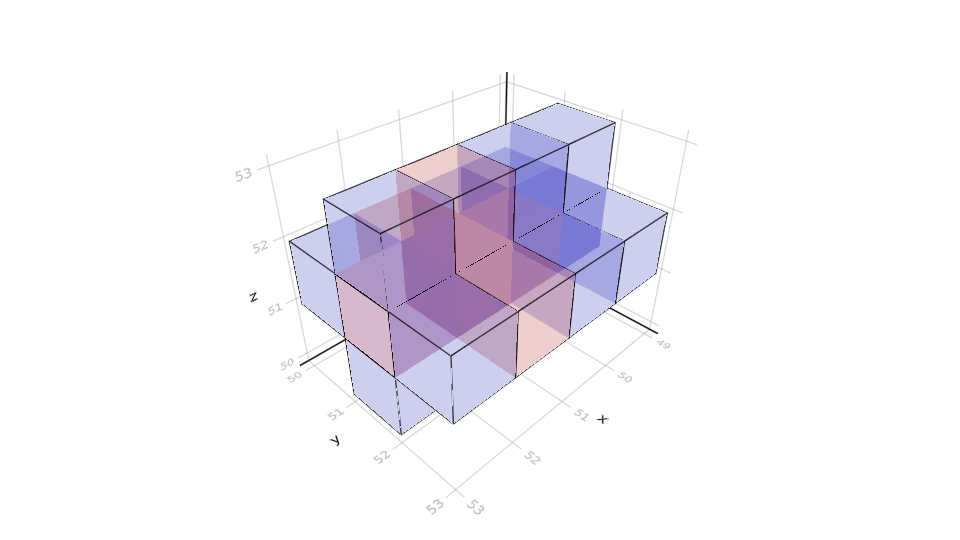
\includegraphics[trim=5cm 0.7cm 5cm 3cm, clip, width=1\linewidth]{algorithm_visualisation/srgcache4/srgcache_step0.png}\\
  \rightline{\color{gray} practice}
\end{frame}
\begin{frame}{\insertsubsection (simplified = 4 Byte) : round 2}
  \centering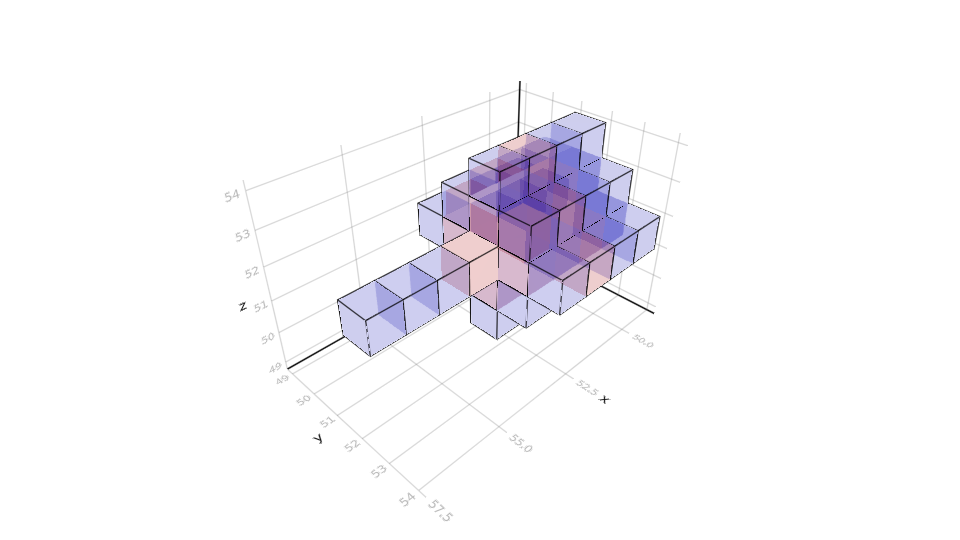
\includegraphics[trim=5cm 0.7cm 5cm 3cm, clip, width=1\linewidth]{algorithm_visualisation/srgcache4/srgcache_step1.png}\\
  \rightline{\color{gray} practice}
\end{frame}
\begin{frame}{\insertsubsection (simplified = 4 Byte) : round 3}
  \centering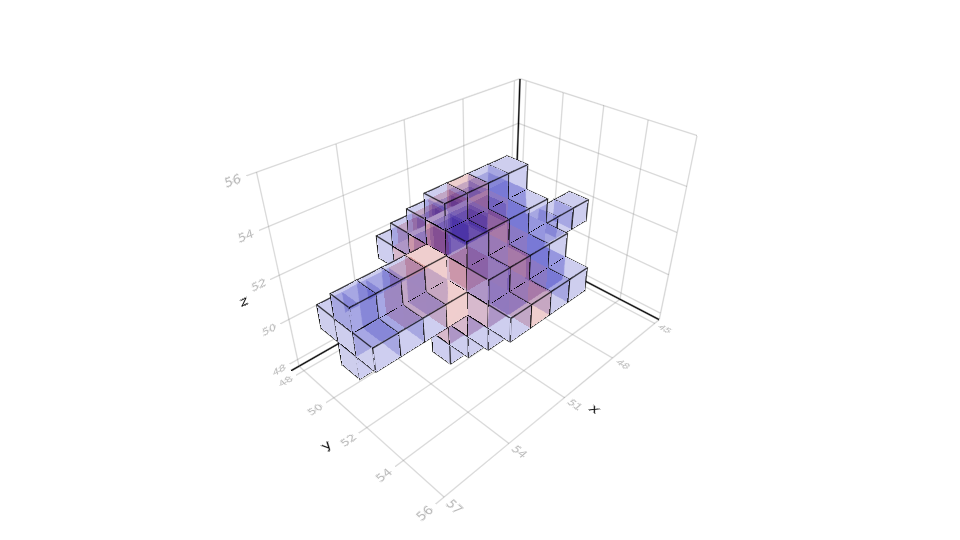
\includegraphics[trim=5cm 0.7cm 5cm 3cm, clip, width=1\linewidth]{algorithm_visualisation/srgcache4/srgcache_step2.png}\\
  \rightline{\color{gray} practice}
\end{frame}
\begin{frame}{\insertsubsection (simplified = 4 Byte) : round 5}
  \centering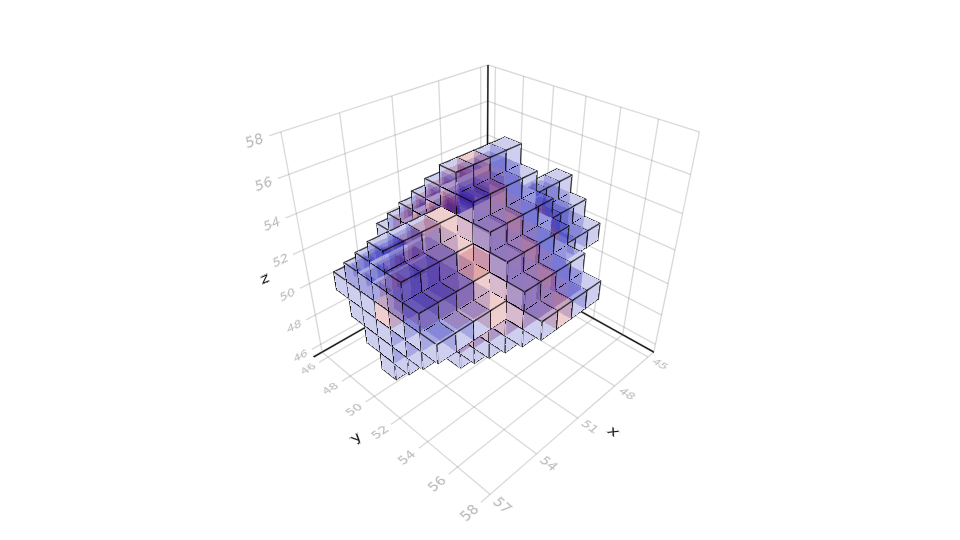
\includegraphics[trim=5cm 0.7cm 5cm 3cm, clip, width=1\linewidth]{algorithm_visualisation/srgcache4/srgcache_step4.png}\\
  \rightline{\color{gray} practice}
\end{frame}
\begin{frame}{\insertsubsection (simplified = 4 Byte) : round 9}
  \centering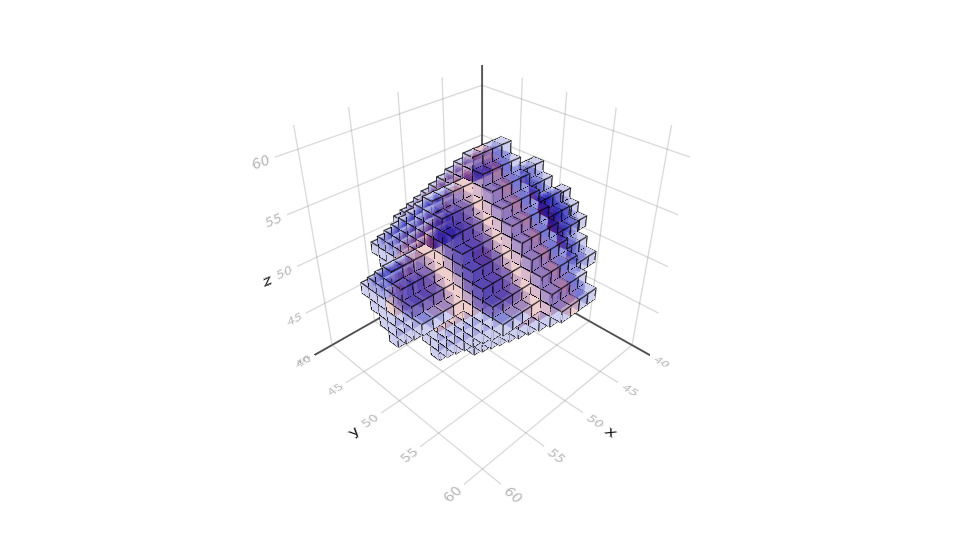
\includegraphics[trim=5cm 0.7cm 5cm 3cm, clip, width=1\linewidth]{algorithm_visualisation/srgcache4/srgcache_step8.png}\\
  \rightline{\color{gray} practice}
\end{frame}
\begin{frame}{\insertsubsection (simplified = 4 Byte) : round 13}
  \centering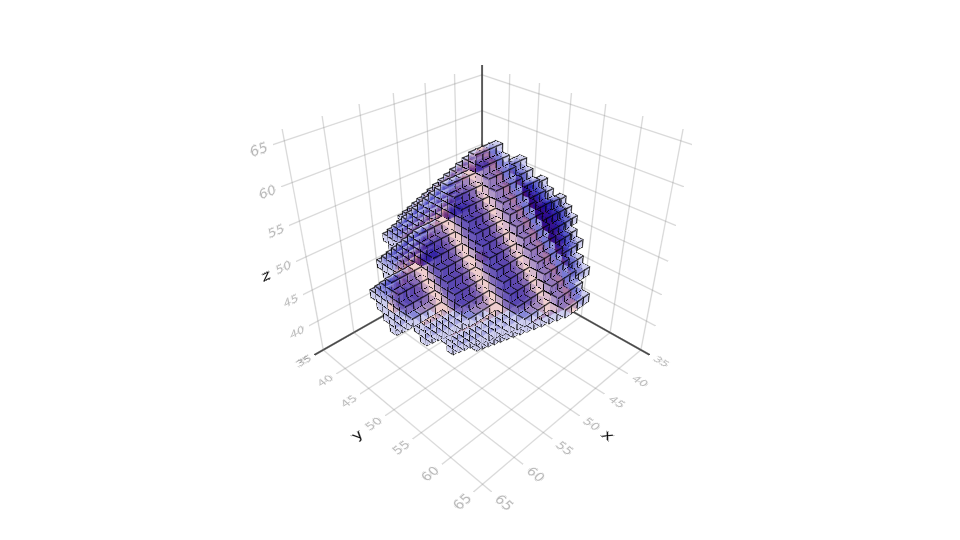
\includegraphics[trim=5cm 0.7cm 5cm 3cm, clip, width=1\linewidth]{algorithm_visualisation/srgcache4/srgcache_step12.png}\\
  \textbf{notable overhead}, visualization out of memory\\
  \rightline{\color{gray} practice}
\end{frame}
\begin{frame}{\insertsubsection (real = 64 Byte) : round 1}
  \centering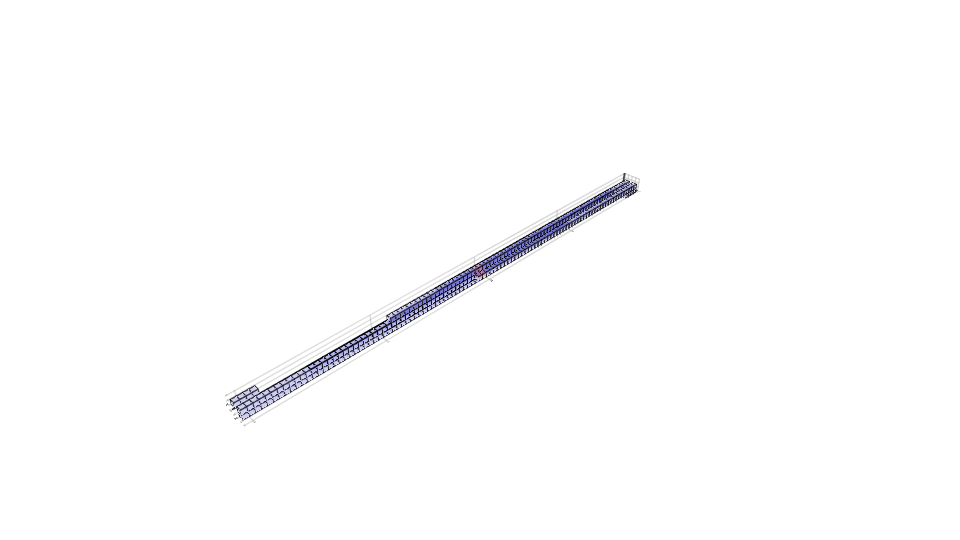
\includegraphics[trim=5cm 0.7cm 5cm 3cm, clip, width=1\linewidth]{algorithm_visualisation/srgcache64/srgcache_step0.png}\\
  \rightline{\color{gray} practice}
\end{frame}
\begin{frame}{\insertsubsection (real = 64 Byte) : round 2}
  \centering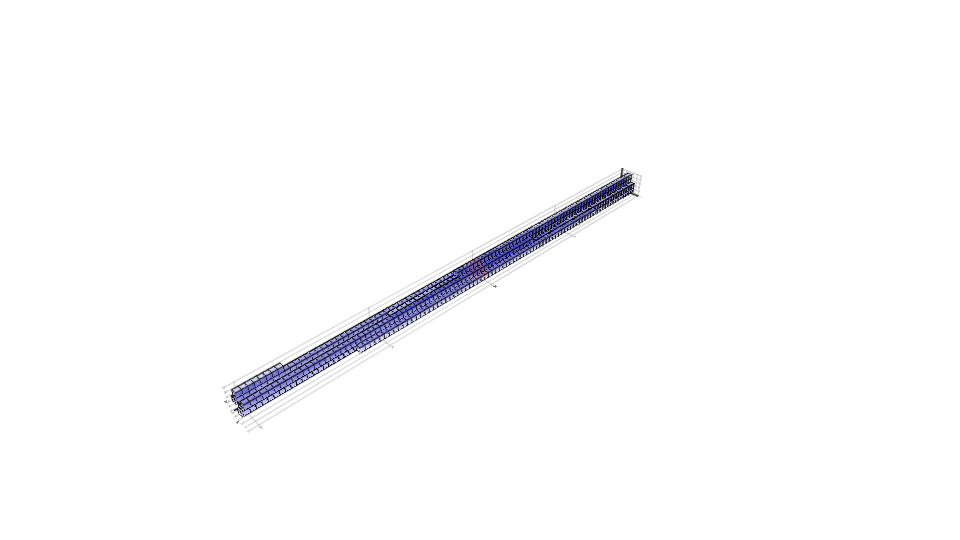
\includegraphics[trim=5cm 0.7cm 5cm 3cm, clip, width=1\linewidth]{algorithm_visualisation/srgcache64/srgcache_step1.png}\\
  \rightline{\color{gray} practice}
\end{frame}
\begin{frame}{\insertsubsection (real = 64 Byte) : round 3}
  \centering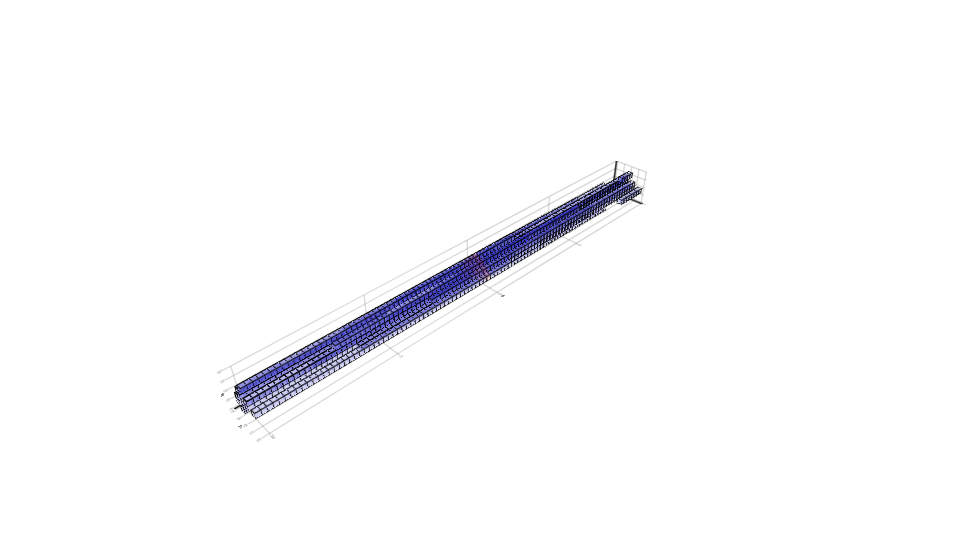
\includegraphics[trim=5cm 0.7cm 5cm 3cm, clip, width=1\linewidth]{algorithm_visualisation/srgcache64/srgcache_step2.png}\\
  \textbf{high overhead}, visualization out of memory\\
  \rightline{\color{gray} practice}
\end{frame}
\begin{frame}{\insertsubsection (approximation)}
  1.1 (shown in our paper) Worst case surface: $O_\text{max} = a^2+2$, $a$ edge length of Cube\\
  1.2 (shown in our paper) surface doubles in every round\\
  1.3 $a=[200,400,800] \Rightarrow O_\text{max} = [40\_000,160\_000,640\_000]$ voxel\\
  \vspace{0.3cm}
  2.1 position of surface voxel in queue: 12 Byte\\
  2.2 due to 1.2: 64 byte(2x)\\
  2.3 $\frac{\text{L3 cache size}}{\text{memory per Voxel}}=\frac{32\text{MB}}{2*64+12\text{B}} = \frac{32\text{MB}}{140\text{B}} = 239\_674 \approx 489^2$\\
  \vspace{0.3cm}
  %3.1 ignore that L3 cache is physically addressed (pages as continous chunks of 4KB or 4MB size mapping to RAM region)\\
  3.1 ignore overhead for cache management (highly architecture dependent\footnote{Patterson and Hennessey Computer Organisation and Design, example \url{https://stackoverflow.com/a/12505900}})\\
  3.2 ignore unknown influence of other processes, Kernel, ...\\
  3.3 ignore small sizes and tips of octahedron (near min/max of y and z of the algorithm surface)
\end{frame}

%\begin{frame}{\Ac{srg} with~\ac{mad} annotated}
%\centering
%\SetAlCapNameFnt{\scriptsize}
%\SetAlCapFnt{\scriptsize}
%\begin{algorithm}[H]
%  \DontPrintSemicolon
%  %\algsetup{linenosize=\scriptsize}
% \scriptsize
%  \caption{\Ac{srg} by Adams and Bischoff} \label{alg:srg}
%  \KwData{Vector \texttt{data} as voxels with values 0(invalid) or 1(valid)}
%  \KwResult{Vector \texttt{data} as voxels with values 0(invalid), 1(unmarked) and 255(marked)}
%  queue.push(seeding\_point); \tcp*{$(x,y,z)$}
%  \While{queue.empty() == false}{
%    first\_element =  queue.front(); \tcp*{$(x,y,z)$, \color{red}\ac{mad}}
%    queue.pop(); \\
%    \ForAll{neighbors of first\_element}{
%      \tcc*{neighbor $\in \{(x\pm 1,y,z),(x,y\pm 1,z),(x,y,z\pm 1)\}$}
%      \If {neighbor $\in \text{Cuboid}(x_\text{max},y_\text{max},z_\text{max})$} {
%        \tcc*{neighbor $(x,y,z)$ is in Cuboid-shaped input data}
%        offset $= x_\text{max}*y_\text{max}*z+x_\text{max}*y+x$;\\
%        neighborValue = \texttt{data}[offset]; \tcp*{\color{red}MAD}
%        \If{neighborValue == 1} {
%          neighborValue = 255;\\
%          queue.push(neighbor);
%        }
%      }
%    }
%  }
%\end{algorithm}
%  It depends, where elements of \textbf{queue} and \textbf{data} are!
%\end{frame}

\subsection{Scan data examples}
\begin{frame}{\insertsubsection: Helixes}
\begin{figure}[h]
\centering
  \begin{subfigure}[t]{0.5\textwidth}
    \centering
  \vskip 0pt
    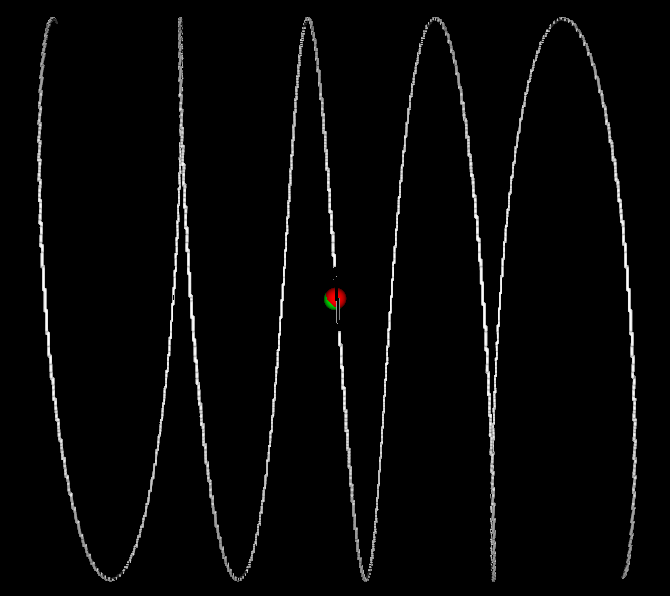
\includegraphics[width=0.9\textwidth]{images/helixd1_800.png}
    \caption{Dilation by Cube with edge length 1.}\label{fig:helixd1_800}
  \end{subfigure}%
  \begin{subfigure}[t]{0.5\textwidth}
    \centering
  \vskip 0pt
    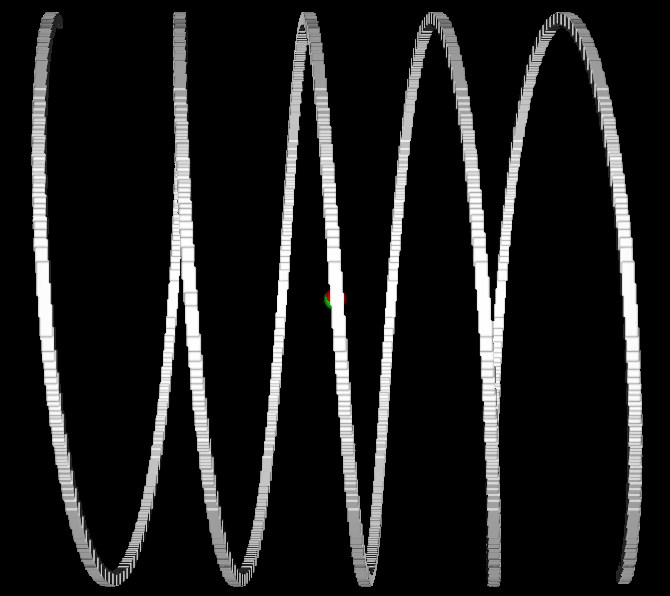
\includegraphics[width=0.9\textwidth]{images/helixd4_800.png}
    \caption{Dilation by Cube with edge length 4.}\label{fig:helixd4_800}
  \end{subfigure}%
  %\caption{Example \texttt{Helix}, size $800\times 800\times 800$}\label{fig:helixes}%
\end{figure}
  edge length: 200, 400 and 800 voxel\\
  reason: measure data-contention (on parallelization) 
\end{frame}

\begin{frame}{\insertsubsection: Maus\_mit\_Draht}
\begin{figure}
\centering
\begin{subfigure}{.5\textwidth}
  \centering
  
\includegraphics[width=.9\linewidth]{images/maus_mit_draht_unprocessed.png}
  \caption{Unprocessed \texttt{maus\_mit\_draht}.}
\end{subfigure}%
\begin{subfigure}{.5\textwidth}
  \centering
  
\includegraphics[width=.9\linewidth]{images/maus_mit_draht_processed.png}
  \caption{Processed \texttt{maus\_mit\_draht}.}
\end{subfigure}
\end{figure}
  reason: measure data-contention (on parallelization) 
\end{frame}

\begin{frame}{\insertsubsection: BoneMaskHigh}
\begin{figure}
\centering
  \begin{subfigure}[b]{.5\textwidth}
  \centering
  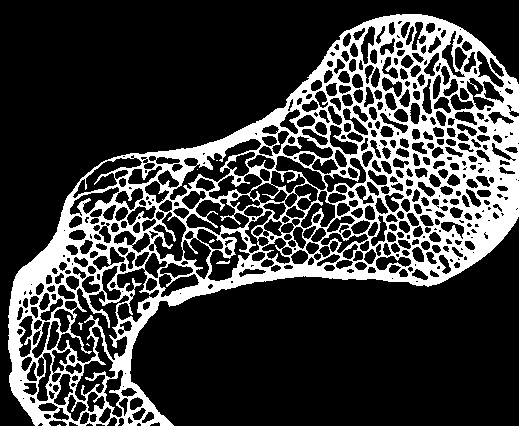
\includegraphics[width=0.9\textwidth]{images/bonemaskhigh_slice_unprocessed.png}
  \caption{Slice of \texttt{BoneMaskHigh}.}
  \end{subfigure}%
  \begin{subfigure}[b]{.5\textwidth}
  \centering
  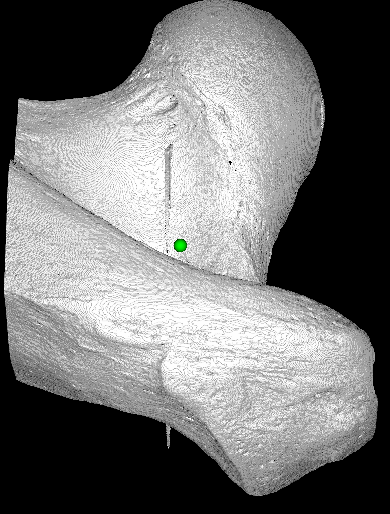
\includegraphics[width=0.9\textwidth]{images/bonemaskhigh_unprocessed.png}
  \caption{3D visualization of \texttt{BoneMaskHigh}.}
  \end{subfigure}
\end{figure}
  reason: relation of forked structures and data-contention (on parallelization)
\end{frame}

\subsection{Results}
\begin{frame}{\Ac{srg} performance}
\centering
\small
\begin{tabularx}{\textwidth}{c|c|c|c|c}
\centering
\textbf{Example} & \textbf{size}[MB] & \textbf{written}[MB] & \textbf{speed}$[\frac{\texttt{voxel}}{\mu s}]$ & \textbf{time}[s]\\
\hline
  Helix\_D1-D5 & 7.63       & 0.007 - 0.177 & 28.1-56.6 & <3.2e-3\\
  Helix\_D1-D5 & 61.04      & 0.014 - 0.356 & 26.8-57.9 & <6.5e-3\\
  Helix\_D1-D5 & 488.28     & 0.03 - 0.72   & 24.5-47.2 & <15e-3 \\
  Maus\_mit\_Draht & 472.88 & 4.9           & 51.5      & 0.10 \\
  BoneMaskHigh & 2028.8     & 134.11        & 19.2      & 7.33
\end{tabularx}
\\
  \vspace{1cm}
  small surface in each~\ac{srg} round $\Rightarrow$ high voxel writing speed ($> 50\frac{\texttt{voxel}}{\mu s}$)\\
  big surface in many~\ac{srg} rounds $\Rightarrow$ small voxel writing speed ($\approx 17\frac{\texttt{voxel}}{\mu s}$)

\end{frame}
\section{Parallelized Seeded Region Growing}
\begin{frame}
  \tableofcontents[currentsection]
\end{frame}
\subsection{Why parallelized Seeded Region Growing?}
\begin{frame}{\insertsubsection}
\centering
  Purpose: Determine and visualize connected voxel of a 3D scan for patient treatment from a user-defined starting point.\\
  \vspace{1cm}
  \begin{enumerate}
      \item simple
      \item fast\textbf{er}: parallelized, \textbf{bigger data sets}
      \item robust
      \item \textbf{in-place} % limit overall memory, so no further volume allocation
  \end{enumerate}
\end{frame}
\subsection{Data-contention between CPU cores}
\begin{frame}{\insertsubsection}
  Cache coherency by current widespread hardware (ARM, Intel, AMD): Every CPU cache must have a valid representation of current data.\\
  Cache line in multiple L1 or L2 cache of other cores: Changes get automatically synchronized.\\
  \vspace{1cm}
\begin{minipage}{0.5\linewidth}
Ideal case of 2 threads\\
  \vspace{0.3cm}
  \includegraphics[width=.95\linewidth]{figures/datacont2.pdf}
\end{minipage}%
\begin{minipage}{0.5\linewidth}
Data contention of 2 threads\\
  \vspace{0.3cm}
  \includegraphics[width=.95\linewidth]{figures/datacont1.pdf}
\end{minipage}%
\end{frame}
\begin{frame}{\insertsubsection : step 1}
\centering
\begin{minipage}{0.5\linewidth}
\begin{figure}[h]%
  \begin{subfigure}[b]{\linewidth}%
  \includegraphics[width=.95\linewidth]{figures/datacontAbad1.pdf}
  \end{subfigure}\\
  \vspace{1cm}
  \begin{subfigure}[b]{\linewidth}%
  \includegraphics[width=.95\linewidth]{figures/datacontAbad2.pdf}
  \end{subfigure}%
  \caption{Thread A}
\end{figure}%
\end{minipage}%
\begin{minipage}{0.5\linewidth}
\begin{figure}[h]%
  \begin{subfigure}[b]{\linewidth}%
  \includegraphics[width=.95\linewidth]{figures/datacontBbad1.pdf}
  \end{subfigure}\\
  \vspace{1cm}
  \begin{subfigure}[b]{\linewidth}%
  \includegraphics[width=.95\linewidth]{figures/datacontBbad2.pdf}
  \end{subfigure}%
  \caption{Thread B}
\end{figure}%
\end{minipage}
\end{frame}
\begin{frame}{\insertsubsection : step 2}
\centering
\begin{minipage}{0.5\linewidth}
\begin{figure}[h]%
  \begin{subfigure}[b]{\linewidth}%
  \includegraphics[width=.95\linewidth]{figures/datacontAbad2.pdf}
  \end{subfigure}\\
  \vspace{1cm}
  \begin{subfigure}[b]{\linewidth}%
  \includegraphics[width=.95\linewidth]{figures/datacontAbad3.pdf}
  \end{subfigure}%
  \caption{Thread A}
\end{figure}%
\end{minipage}%
\begin{minipage}{0.5\linewidth}
\begin{figure}[h]%
  \begin{subfigure}[b]{\linewidth}%
  \includegraphics[width=.95\linewidth]{figures/datacontBbad2.pdf}
  \end{subfigure}\\
  \vspace{1cm}
  \begin{subfigure}[b]{\linewidth}%
  \includegraphics[width=.95\linewidth]{figures/datacontBbad3.pdf}
  \end{subfigure}%
  \caption{Thread B}
\end{figure}%
\end{minipage}
\end{frame}
\begin{frame}{\insertsubsection : step 3}
\centering
\begin{minipage}{0.5\linewidth}
\begin{figure}[h]%
  \begin{subfigure}[b]{\linewidth}%
  \includegraphics[width=.95\linewidth]{figures/datacontAbad3.pdf}
  \end{subfigure}\\
  \vspace{1cm}
  \begin{subfigure}[b]{\linewidth}%
  \includegraphics[width=.95\linewidth]{figures/datacontAbad4.pdf}
  \end{subfigure}%
  \caption{Thread A}
\end{figure}%
\end{minipage}%
\begin{minipage}{0.5\linewidth}
\begin{figure}[h]%
  \begin{subfigure}[b]{\linewidth}%
  \includegraphics[width=.95\linewidth]{figures/datacontBbad3.pdf}
  \end{subfigure}\\
  \vspace{1cm}
  \begin{subfigure}[b]{\linewidth}%
  \includegraphics[width=.95\linewidth]{figures/datacontBbad4.pdf}
  \end{subfigure}%
  \caption{Thread B}
\end{figure}%
\end{minipage}
\end{frame}
\begin{frame}{\insertsubsection : step 4}
\centering
\begin{minipage}{0.5\linewidth}
\begin{figure}[h]%
  \begin{subfigure}[b]{\linewidth}%
  \includegraphics[width=.95\linewidth]{figures/datacontAbad4.pdf}
  \end{subfigure}\\
  \vspace{1cm}
  \begin{subfigure}[b]{\linewidth}%
  \includegraphics[width=.95\linewidth]{figures/datacontAbad5.pdf}
  \end{subfigure}%
  \caption{Thread A}
\end{figure}%
\end{minipage}%
\begin{minipage}{0.5\linewidth}
\begin{figure}[h]%
  \begin{subfigure}[b]{\linewidth}%
  \includegraphics[width=.95\linewidth]{figures/datacontBbad4.pdf}
  \end{subfigure}\\
  \vspace{1cm}
  \begin{subfigure}[b]{\linewidth}%
  \includegraphics[width=.95\linewidth]{figures/datacontBbad5.pdf}
  \end{subfigure}%
  \caption{Thread B}
\end{figure}%
\end{minipage}
forwarding data results in processing delay
\end{frame}
\begin{frame}{\insertsubsection : step 5}
\centering
\begin{minipage}{0.5\linewidth}
\begin{figure}[h]%
  \begin{subfigure}[b]{\linewidth}%
  \includegraphics[width=.95\linewidth]{figures/datacontAbad5.pdf}
  \end{subfigure}\\
  \vspace{1cm}
  \begin{subfigure}[b]{\linewidth}%
  \includegraphics[width=.95\linewidth]{figures/datacontAbad6.pdf}
  \end{subfigure}%
  \caption{Thread A}
\end{figure}%
\end{minipage}%
\begin{minipage}{0.5\linewidth}
\begin{figure}[h]%
  \begin{subfigure}[b]{\linewidth}%
  \includegraphics[width=.95\linewidth]{figures/datacontBbad5.pdf}
  \end{subfigure}\\
  \vspace{1cm}
  \begin{subfigure}[b]{\linewidth}%
  \includegraphics[width=.95\linewidth]{figures/datacontBbad6.pdf}
  \end{subfigure}%
  \caption{Thread B}
\end{figure}%
\end{minipage}
forwarding data results in processing delay, AGAIN...
\end{frame}
\subsection{\texttt{simple parallel Seeded Region Growing (simpaSRG)}}
\begin{frame}{\insertsubsection}
  Idea for~\ac{simpa}: 
  \begin{enumerate}
    \item Every 1000 successfull voxel markings, try to start a new thread with~\ac{srg}.
    \item Every thread with~\ac{srg} works independent and deactivates itself, when finding no valid voxels.
  \end{enumerate}
\end{frame}
\begin{frame}{\texttt{simpaSRG} : round 0}
  %\vspace{-0.5cm}
\includegraphics[trim=5cm 0.7cm 5cm 3cm, clip, width=1\linewidth]{algorithm_visualisation/srgthreads2/srg2threads0.png}\\
  \rightline{\color{gray} theory}
\end{frame}
\begin{frame}{\texttt{simpaSRG} : round 1}
  %\vspace{-0.5cm}
\includegraphics[trim=5cm 0.7cm 5cm 3cm, clip, width=1\linewidth]{algorithm_visualisation/srgthreads2/srg2threads1.png}\\
  \rightline{\color{gray} theory}
\end{frame}
\begin{frame}{\texttt{simpaSRG} : round 2}
  %\vspace{-0.5cm}
\includegraphics[trim=5cm 0.7cm 5cm 3cm, clip, width=1\linewidth]{algorithm_visualisation/srgthreads2/srg2threads2.png}\\
  \rightline{\color{gray} theory}
\end{frame}
\begin{frame}{\texttt{simpaSRG} : round 3}
  %\vspace{-0.5cm}
\includegraphics[trim=5cm 0.7cm 5cm 3cm, clip, width=1\linewidth]{algorithm_visualisation/srgthreads2/srg2threads3.png}\\
  \rightline{\color{gray} theory}
\end{frame}
\begin{frame}{\texttt{simpaSRG} : round 4}
  %\vspace{-0.5cm}
\includegraphics[trim=5cm 0.7cm 5cm 3cm, clip, width=1\linewidth]{algorithm_visualisation/srgthreads2/srg2threads4.png}\\
  \rightline{\color{gray} theory}
\end{frame}
\begin{frame}{\texttt{simpaSRG} : round 5}
  %\vspace{-0.5cm}
\includegraphics[trim=5cm 0.7cm 5cm 3cm, clip, width=1\linewidth]{algorithm_visualisation/srgthreads2/srg2threads5.png}\\
  red voxel: new thread with SRG \rightline{\color{gray} theory}
\end{frame}
\begin{frame}{\texttt{simpaSRG} : round 6}
  %\vspace{-0.5cm}
\includegraphics[trim=5cm 0.7cm 5cm 3cm, clip, width=1\linewidth]{algorithm_visualisation/srgthreads2/srg2threads6.png}\\
  \rightline{\color{gray} theory}
\end{frame}
\begin{frame}{\texttt{simpaSRG} : round 7}
  %\vspace{-0.5cm}
\includegraphics[trim=5cm 0.7cm 5cm 3cm, clip, width=1\linewidth]{algorithm_visualisation/srgthreads2/srg2threads7.png}\\
  \rightline{\color{gray} theory}
\end{frame}
\begin{frame}{\texttt{simpaSRG} : round 8}
  %\vspace{-0.5cm}
\includegraphics[trim=5cm 0.7cm 5cm 3cm, clip, width=1\linewidth]{algorithm_visualisation/srgthreads2/srg2threads8.png}\\
  \rightline{\color{gray} theory}
\end{frame}
\begin{frame}{\texttt{simpaSRG} : round 9}
  %\vspace{-0.5cm}
\includegraphics[trim=5cm 0.7cm 5cm 3cm, clip, width=1\linewidth]{algorithm_visualisation/srgthreads2/srg2threads9.png}\\
  smaller surface of red SRG $\Rightarrow$ faster growing\\
	\rightline{\color{gray} theory}
\end{frame}
\begin{frame}{\texttt{simpaSRG} : round 10}
  %\vspace{-0.5cm}
\includegraphics[trim=5cm 0.7cm 5cm 3cm, clip, width=1\linewidth]{algorithm_visualisation/srgthreads2/srg2threads10.png}\\
  \rightline{\color{gray} theory}
\end{frame}
\begin{frame}{\texttt{simpaSRG} : round 11}
  %\vspace{-0.5cm}
\includegraphics[trim=5cm 0.7cm 5cm 3cm, clip, width=1\linewidth]{algorithm_visualisation/srgthreads2/srg2threads11.png}\\
  \rightline{\color{gray} theory}
\end{frame}
%\SetAlCapNameFnt{\tiny}
%\SetAlCapFnt{\tiny}
%\SetKwProg{Fn}{Function}{}{end}
%\SetKwFunction{FnWatcher}{FnWatcherThread}%
%\SetKwFunction{FnWorker}{FnWorkerThread}%
%\SetKwFunction{Deactivate}{DeactivateCurrentThread}%
%\SetAlgoLongEnd
%\begin{algorithm}[H]
%  \DontPrintSemicolon
%  \caption{\acf{simpa} 1/2} \label{alg:srgpar}
%  \tiny
%  \KwData{Vector \texttt{data} as voxels with values 0(invalid) or 1(valid)}
%  \KwResult{Vector \texttt{data} as voxels with values 0(invalid), 1(unmarked) and 255(marked)}
%  \Fn(){\FnWatcher{seedpoint,data,$\ldots$}}{
%    read\_data\_from\_disk(); \\
%    start \FnWorker() in new thread; \\
%    \While{AnyWorkerThread.running == true}{
%      sleep\_for\_100milliseconds();
%    }
%    save\_data\_to\_disk();
%  }
%  %
%\end{algorithm}
%\end{frame}
%\begin{frame}{\insertsubsection (2/2)}
%\centering
%\SetAlCapNameFnt{\tiny}
%\SetAlCapFnt{\tiny}
%\SetKwProg{Fn}{Function}{}{end}
%\SetKwFunction{FnWatcher}{FnWatcherThread}%
%\SetKwFunction{FnWorker}{FnWorkerThread}%
%\SetKwFunction{Deactivate}{DeactivateCurrentThread}%
%\SetAlgoLongEnd
%\begin{algorithm}[H]
%  \DontPrintSemicolon
%  \caption{\acf{simpa} 2/2} \label{alg:srgpar}
%  \tiny
%  \KwData{Vector \texttt{data} as voxels with values 0(invalid) or 1(valid)}
%  \KwResult{Vector \texttt{data} as voxels with values 0(invalid), 1(unmarked) and 255(marked)}
%  \Fn(){\FnWorker{seedpoint,data,$\ldots$}}{
%    queue.push(seeding\_point); \\
%    countdown = 1000; \\
%    \While{queue.empty() == false}{
%      first\_element =  queue.front(); \tcp*{$(x,y,z)$, \color{red}\ac{mad}}
%      queue.pop(); \\
%      \ForAll{neighbors of first\_element}{
%        \tcc*{neighbor $\in \{(x\pm 1,y,z),(x,y\pm 1,z),(x,y,z\pm 1)\}$}
%        \If {neighbor $\in \text{Cuboid}(x_\text{max},y_\text{max},z_\text{max})$} {
%          \tcc*{neighbor $(x,y,z)$ is in Cuboid-shaped input data}
%          offset $= x_\text{max}*y_\text{max}*z+x_\text{max}*y+x$;\\
%          neighborValue = \texttt{data}[offset]; \tcp*{\color{red}MAD}
%          \If{neighborValue == 1} {
%            \eIf{countdown == 0}{
%              countdown = 1000; \\
%              \If{try\_to\_start\_\FnWorker() == failure}{
%                neighborValue = 255; \\
%                queue.push(neighbor); \\
%                countdown = countdown-1;
%              }
%            }%else
%            {
%              neighborValue = 255; \\
%              queue.push(neighbor); \\
%              countdown = countdown-1;
%            }
%          }
%        }
%      }
%    }
%    \Deactivate();
%  }
%  %
%\end{algorithm}
%\end{frame}
\subsection{Results}
\begin{frame}{Result for Helixes}
  \begin{adjustbox}{max totalsize={.9\textwidth}{.9\textheight},center}
    {%% Creator: Matplotlib, PGF backend
%%
%% To include the figure in your LaTeX document, write
%%   \input{<filename>.pgf}
%%
%% Make sure the required packages are loaded in your preamble
%%   \usepackage{pgf}
%%
%% and, on pdftex
%%   \usepackage[utf8]{inputenc}\DeclareUnicodeCharacter{2212}{-}
%%
%% or, on luatex and xetex
%%   \usepackage{unicode-math}
%%
%% Figures using additional raster images can only be included by \input if
%% they are in the same directory as the main LaTeX file. For loading figures
%% from other directories you can use the `import` package
%%   \usepackage{import}
%%
%% and then include the figures with
%%   \import{<path to file>}{<filename>.pgf}
%%
%% Matplotlib used the following preamble
%%   \usepackage{fontspec}
%%
\begingroup%
\makeatletter%
\begin{pgfpicture}%
\pgfpathrectangle{\pgfpointorigin}{\pgfqpoint{2.900852in}{3.692771in}}%
\pgfusepath{use as bounding box, clip}%
\begin{pgfscope}%
\pgfsetbuttcap%
\pgfsetmiterjoin%
\definecolor{currentfill}{rgb}{1.000000,1.000000,1.000000}%
\pgfsetfillcolor{currentfill}%
\pgfsetlinewidth{0.000000pt}%
\definecolor{currentstroke}{rgb}{1.000000,1.000000,1.000000}%
\pgfsetstrokecolor{currentstroke}%
\pgfsetdash{}{0pt}%
\pgfpathmoveto{\pgfqpoint{0.000000in}{0.000000in}}%
\pgfpathlineto{\pgfqpoint{2.900852in}{0.000000in}}%
\pgfpathlineto{\pgfqpoint{2.900852in}{3.692771in}}%
\pgfpathlineto{\pgfqpoint{0.000000in}{3.692771in}}%
\pgfpathclose%
\pgfusepath{fill}%
\end{pgfscope}%
\begin{pgfscope}%
\pgfsetbuttcap%
\pgfsetmiterjoin%
\definecolor{currentfill}{rgb}{1.000000,1.000000,1.000000}%
\pgfsetfillcolor{currentfill}%
\pgfsetlinewidth{0.000000pt}%
\definecolor{currentstroke}{rgb}{0.000000,0.000000,0.000000}%
\pgfsetstrokecolor{currentstroke}%
\pgfsetstrokeopacity{0.000000}%
\pgfsetdash{}{0pt}%
\pgfpathmoveto{\pgfqpoint{0.306837in}{0.855472in}}%
\pgfpathlineto{\pgfqpoint{2.900852in}{0.855472in}}%
\pgfpathlineto{\pgfqpoint{2.900852in}{3.550472in}}%
\pgfpathlineto{\pgfqpoint{0.306837in}{3.550472in}}%
\pgfpathclose%
\pgfusepath{fill}%
\end{pgfscope}%
\begin{pgfscope}%
\pgfpathrectangle{\pgfqpoint{0.306837in}{0.855472in}}{\pgfqpoint{2.594014in}{2.695000in}}%
\pgfusepath{clip}%
\pgfsetbuttcap%
\pgfsetmiterjoin%
\definecolor{currentfill}{rgb}{0.121569,0.466667,0.705882}%
\pgfsetfillcolor{currentfill}%
\pgfsetlinewidth{0.000000pt}%
\definecolor{currentstroke}{rgb}{0.000000,0.000000,0.000000}%
\pgfsetstrokecolor{currentstroke}%
\pgfsetstrokeopacity{0.000000}%
\pgfsetdash{}{0pt}%
\pgfpathmoveto{\pgfqpoint{0.424747in}{0.855472in}}%
\pgfpathlineto{\pgfqpoint{0.472228in}{0.855472in}}%
\pgfpathlineto{\pgfqpoint{0.472228in}{2.102654in}}%
\pgfpathlineto{\pgfqpoint{0.424747in}{2.102654in}}%
\pgfpathclose%
\pgfusepath{fill}%
\end{pgfscope}%
\begin{pgfscope}%
\pgfpathrectangle{\pgfqpoint{0.306837in}{0.855472in}}{\pgfqpoint{2.594014in}{2.695000in}}%
\pgfusepath{clip}%
\pgfsetbuttcap%
\pgfsetmiterjoin%
\definecolor{currentfill}{rgb}{0.121569,0.466667,0.705882}%
\pgfsetfillcolor{currentfill}%
\pgfsetlinewidth{0.000000pt}%
\definecolor{currentstroke}{rgb}{0.000000,0.000000,0.000000}%
\pgfsetstrokecolor{currentstroke}%
\pgfsetstrokeopacity{0.000000}%
\pgfsetdash{}{0pt}%
\pgfpathmoveto{\pgfqpoint{0.583015in}{0.855472in}}%
\pgfpathlineto{\pgfqpoint{0.630496in}{0.855472in}}%
\pgfpathlineto{\pgfqpoint{0.630496in}{2.041329in}}%
\pgfpathlineto{\pgfqpoint{0.583015in}{2.041329in}}%
\pgfpathclose%
\pgfusepath{fill}%
\end{pgfscope}%
\begin{pgfscope}%
\pgfpathrectangle{\pgfqpoint{0.306837in}{0.855472in}}{\pgfqpoint{2.594014in}{2.695000in}}%
\pgfusepath{clip}%
\pgfsetbuttcap%
\pgfsetmiterjoin%
\definecolor{currentfill}{rgb}{0.121569,0.466667,0.705882}%
\pgfsetfillcolor{currentfill}%
\pgfsetlinewidth{0.000000pt}%
\definecolor{currentstroke}{rgb}{0.000000,0.000000,0.000000}%
\pgfsetstrokecolor{currentstroke}%
\pgfsetstrokeopacity{0.000000}%
\pgfsetdash{}{0pt}%
\pgfpathmoveto{\pgfqpoint{0.741283in}{0.855472in}}%
\pgfpathlineto{\pgfqpoint{0.788764in}{0.855472in}}%
\pgfpathlineto{\pgfqpoint{0.788764in}{1.942018in}}%
\pgfpathlineto{\pgfqpoint{0.741283in}{1.942018in}}%
\pgfpathclose%
\pgfusepath{fill}%
\end{pgfscope}%
\begin{pgfscope}%
\pgfpathrectangle{\pgfqpoint{0.306837in}{0.855472in}}{\pgfqpoint{2.594014in}{2.695000in}}%
\pgfusepath{clip}%
\pgfsetbuttcap%
\pgfsetmiterjoin%
\definecolor{currentfill}{rgb}{0.121569,0.466667,0.705882}%
\pgfsetfillcolor{currentfill}%
\pgfsetlinewidth{0.000000pt}%
\definecolor{currentstroke}{rgb}{0.000000,0.000000,0.000000}%
\pgfsetstrokecolor{currentstroke}%
\pgfsetstrokeopacity{0.000000}%
\pgfsetdash{}{0pt}%
\pgfpathmoveto{\pgfqpoint{0.899551in}{0.855472in}}%
\pgfpathlineto{\pgfqpoint{0.947032in}{0.855472in}}%
\pgfpathlineto{\pgfqpoint{0.947032in}{2.458027in}}%
\pgfpathlineto{\pgfqpoint{0.899551in}{2.458027in}}%
\pgfpathclose%
\pgfusepath{fill}%
\end{pgfscope}%
\begin{pgfscope}%
\pgfpathrectangle{\pgfqpoint{0.306837in}{0.855472in}}{\pgfqpoint{2.594014in}{2.695000in}}%
\pgfusepath{clip}%
\pgfsetbuttcap%
\pgfsetmiterjoin%
\definecolor{currentfill}{rgb}{0.121569,0.466667,0.705882}%
\pgfsetfillcolor{currentfill}%
\pgfsetlinewidth{0.000000pt}%
\definecolor{currentstroke}{rgb}{0.000000,0.000000,0.000000}%
\pgfsetstrokecolor{currentstroke}%
\pgfsetstrokeopacity{0.000000}%
\pgfsetdash{}{0pt}%
\pgfpathmoveto{\pgfqpoint{1.057820in}{0.855472in}}%
\pgfpathlineto{\pgfqpoint{1.105300in}{0.855472in}}%
\pgfpathlineto{\pgfqpoint{1.105300in}{2.767943in}}%
\pgfpathlineto{\pgfqpoint{1.057820in}{2.767943in}}%
\pgfpathclose%
\pgfusepath{fill}%
\end{pgfscope}%
\begin{pgfscope}%
\pgfpathrectangle{\pgfqpoint{0.306837in}{0.855472in}}{\pgfqpoint{2.594014in}{2.695000in}}%
\pgfusepath{clip}%
\pgfsetbuttcap%
\pgfsetmiterjoin%
\definecolor{currentfill}{rgb}{0.121569,0.466667,0.705882}%
\pgfsetfillcolor{currentfill}%
\pgfsetlinewidth{0.000000pt}%
\definecolor{currentstroke}{rgb}{0.000000,0.000000,0.000000}%
\pgfsetstrokecolor{currentstroke}%
\pgfsetstrokeopacity{0.000000}%
\pgfsetdash{}{0pt}%
\pgfpathmoveto{\pgfqpoint{1.216088in}{0.855472in}}%
\pgfpathlineto{\pgfqpoint{1.263568in}{0.855472in}}%
\pgfpathlineto{\pgfqpoint{1.263568in}{2.420640in}}%
\pgfpathlineto{\pgfqpoint{1.216088in}{2.420640in}}%
\pgfpathclose%
\pgfusepath{fill}%
\end{pgfscope}%
\begin{pgfscope}%
\pgfpathrectangle{\pgfqpoint{0.306837in}{0.855472in}}{\pgfqpoint{2.594014in}{2.695000in}}%
\pgfusepath{clip}%
\pgfsetbuttcap%
\pgfsetmiterjoin%
\definecolor{currentfill}{rgb}{0.121569,0.466667,0.705882}%
\pgfsetfillcolor{currentfill}%
\pgfsetlinewidth{0.000000pt}%
\definecolor{currentstroke}{rgb}{0.000000,0.000000,0.000000}%
\pgfsetstrokecolor{currentstroke}%
\pgfsetstrokeopacity{0.000000}%
\pgfsetdash{}{0pt}%
\pgfpathmoveto{\pgfqpoint{1.374356in}{0.855472in}}%
\pgfpathlineto{\pgfqpoint{1.421836in}{0.855472in}}%
\pgfpathlineto{\pgfqpoint{1.421836in}{2.969514in}}%
\pgfpathlineto{\pgfqpoint{1.374356in}{2.969514in}}%
\pgfpathclose%
\pgfusepath{fill}%
\end{pgfscope}%
\begin{pgfscope}%
\pgfpathrectangle{\pgfqpoint{0.306837in}{0.855472in}}{\pgfqpoint{2.594014in}{2.695000in}}%
\pgfusepath{clip}%
\pgfsetbuttcap%
\pgfsetmiterjoin%
\definecolor{currentfill}{rgb}{0.121569,0.466667,0.705882}%
\pgfsetfillcolor{currentfill}%
\pgfsetlinewidth{0.000000pt}%
\definecolor{currentstroke}{rgb}{0.000000,0.000000,0.000000}%
\pgfsetstrokecolor{currentstroke}%
\pgfsetstrokeopacity{0.000000}%
\pgfsetdash{}{0pt}%
\pgfpathmoveto{\pgfqpoint{1.532624in}{0.855472in}}%
\pgfpathlineto{\pgfqpoint{1.580104in}{0.855472in}}%
\pgfpathlineto{\pgfqpoint{1.580104in}{2.737334in}}%
\pgfpathlineto{\pgfqpoint{1.532624in}{2.737334in}}%
\pgfpathclose%
\pgfusepath{fill}%
\end{pgfscope}%
\begin{pgfscope}%
\pgfpathrectangle{\pgfqpoint{0.306837in}{0.855472in}}{\pgfqpoint{2.594014in}{2.695000in}}%
\pgfusepath{clip}%
\pgfsetbuttcap%
\pgfsetmiterjoin%
\definecolor{currentfill}{rgb}{0.121569,0.466667,0.705882}%
\pgfsetfillcolor{currentfill}%
\pgfsetlinewidth{0.000000pt}%
\definecolor{currentstroke}{rgb}{0.000000,0.000000,0.000000}%
\pgfsetstrokecolor{currentstroke}%
\pgfsetstrokeopacity{0.000000}%
\pgfsetdash{}{0pt}%
\pgfpathmoveto{\pgfqpoint{1.690892in}{0.855472in}}%
\pgfpathlineto{\pgfqpoint{1.738372in}{0.855472in}}%
\pgfpathlineto{\pgfqpoint{1.738372in}{2.755912in}}%
\pgfpathlineto{\pgfqpoint{1.690892in}{2.755912in}}%
\pgfpathclose%
\pgfusepath{fill}%
\end{pgfscope}%
\begin{pgfscope}%
\pgfpathrectangle{\pgfqpoint{0.306837in}{0.855472in}}{\pgfqpoint{2.594014in}{2.695000in}}%
\pgfusepath{clip}%
\pgfsetbuttcap%
\pgfsetmiterjoin%
\definecolor{currentfill}{rgb}{0.121569,0.466667,0.705882}%
\pgfsetfillcolor{currentfill}%
\pgfsetlinewidth{0.000000pt}%
\definecolor{currentstroke}{rgb}{0.000000,0.000000,0.000000}%
\pgfsetstrokecolor{currentstroke}%
\pgfsetstrokeopacity{0.000000}%
\pgfsetdash{}{0pt}%
\pgfpathmoveto{\pgfqpoint{1.849160in}{0.855472in}}%
\pgfpathlineto{\pgfqpoint{1.896640in}{0.855472in}}%
\pgfpathlineto{\pgfqpoint{1.896640in}{3.122762in}}%
\pgfpathlineto{\pgfqpoint{1.849160in}{3.122762in}}%
\pgfpathclose%
\pgfusepath{fill}%
\end{pgfscope}%
\begin{pgfscope}%
\pgfpathrectangle{\pgfqpoint{0.306837in}{0.855472in}}{\pgfqpoint{2.594014in}{2.695000in}}%
\pgfusepath{clip}%
\pgfsetbuttcap%
\pgfsetmiterjoin%
\definecolor{currentfill}{rgb}{0.121569,0.466667,0.705882}%
\pgfsetfillcolor{currentfill}%
\pgfsetlinewidth{0.000000pt}%
\definecolor{currentstroke}{rgb}{0.000000,0.000000,0.000000}%
\pgfsetstrokecolor{currentstroke}%
\pgfsetstrokeopacity{0.000000}%
\pgfsetdash{}{0pt}%
\pgfpathmoveto{\pgfqpoint{2.007428in}{0.855472in}}%
\pgfpathlineto{\pgfqpoint{2.054909in}{0.855472in}}%
\pgfpathlineto{\pgfqpoint{2.054909in}{2.923467in}}%
\pgfpathlineto{\pgfqpoint{2.007428in}{2.923467in}}%
\pgfpathclose%
\pgfusepath{fill}%
\end{pgfscope}%
\begin{pgfscope}%
\pgfpathrectangle{\pgfqpoint{0.306837in}{0.855472in}}{\pgfqpoint{2.594014in}{2.695000in}}%
\pgfusepath{clip}%
\pgfsetbuttcap%
\pgfsetmiterjoin%
\definecolor{currentfill}{rgb}{0.121569,0.466667,0.705882}%
\pgfsetfillcolor{currentfill}%
\pgfsetlinewidth{0.000000pt}%
\definecolor{currentstroke}{rgb}{0.000000,0.000000,0.000000}%
\pgfsetstrokecolor{currentstroke}%
\pgfsetstrokeopacity{0.000000}%
\pgfsetdash{}{0pt}%
\pgfpathmoveto{\pgfqpoint{2.165696in}{0.855472in}}%
\pgfpathlineto{\pgfqpoint{2.213177in}{0.855472in}}%
\pgfpathlineto{\pgfqpoint{2.213177in}{2.961080in}}%
\pgfpathlineto{\pgfqpoint{2.165696in}{2.961080in}}%
\pgfpathclose%
\pgfusepath{fill}%
\end{pgfscope}%
\begin{pgfscope}%
\pgfpathrectangle{\pgfqpoint{0.306837in}{0.855472in}}{\pgfqpoint{2.594014in}{2.695000in}}%
\pgfusepath{clip}%
\pgfsetbuttcap%
\pgfsetmiterjoin%
\definecolor{currentfill}{rgb}{0.121569,0.466667,0.705882}%
\pgfsetfillcolor{currentfill}%
\pgfsetlinewidth{0.000000pt}%
\definecolor{currentstroke}{rgb}{0.000000,0.000000,0.000000}%
\pgfsetstrokecolor{currentstroke}%
\pgfsetstrokeopacity{0.000000}%
\pgfsetdash{}{0pt}%
\pgfpathmoveto{\pgfqpoint{2.323964in}{0.855472in}}%
\pgfpathlineto{\pgfqpoint{2.371445in}{0.855472in}}%
\pgfpathlineto{\pgfqpoint{2.371445in}{3.363855in}}%
\pgfpathlineto{\pgfqpoint{2.323964in}{3.363855in}}%
\pgfpathclose%
\pgfusepath{fill}%
\end{pgfscope}%
\begin{pgfscope}%
\pgfpathrectangle{\pgfqpoint{0.306837in}{0.855472in}}{\pgfqpoint{2.594014in}{2.695000in}}%
\pgfusepath{clip}%
\pgfsetbuttcap%
\pgfsetmiterjoin%
\definecolor{currentfill}{rgb}{0.121569,0.466667,0.705882}%
\pgfsetfillcolor{currentfill}%
\pgfsetlinewidth{0.000000pt}%
\definecolor{currentstroke}{rgb}{0.000000,0.000000,0.000000}%
\pgfsetstrokecolor{currentstroke}%
\pgfsetstrokeopacity{0.000000}%
\pgfsetdash{}{0pt}%
\pgfpathmoveto{\pgfqpoint{2.482232in}{0.855472in}}%
\pgfpathlineto{\pgfqpoint{2.529713in}{0.855472in}}%
\pgfpathlineto{\pgfqpoint{2.529713in}{3.422139in}}%
\pgfpathlineto{\pgfqpoint{2.482232in}{3.422139in}}%
\pgfpathclose%
\pgfusepath{fill}%
\end{pgfscope}%
\begin{pgfscope}%
\pgfpathrectangle{\pgfqpoint{0.306837in}{0.855472in}}{\pgfqpoint{2.594014in}{2.695000in}}%
\pgfusepath{clip}%
\pgfsetbuttcap%
\pgfsetmiterjoin%
\definecolor{currentfill}{rgb}{0.121569,0.466667,0.705882}%
\pgfsetfillcolor{currentfill}%
\pgfsetlinewidth{0.000000pt}%
\definecolor{currentstroke}{rgb}{0.000000,0.000000,0.000000}%
\pgfsetstrokecolor{currentstroke}%
\pgfsetstrokeopacity{0.000000}%
\pgfsetdash{}{0pt}%
\pgfpathmoveto{\pgfqpoint{2.640501in}{0.855472in}}%
\pgfpathlineto{\pgfqpoint{2.687981in}{0.855472in}}%
\pgfpathlineto{\pgfqpoint{2.687981in}{2.949198in}}%
\pgfpathlineto{\pgfqpoint{2.640501in}{2.949198in}}%
\pgfpathclose%
\pgfusepath{fill}%
\end{pgfscope}%
\begin{pgfscope}%
\pgfpathrectangle{\pgfqpoint{0.306837in}{0.855472in}}{\pgfqpoint{2.594014in}{2.695000in}}%
\pgfusepath{clip}%
\pgfsetbuttcap%
\pgfsetmiterjoin%
\definecolor{currentfill}{rgb}{1.000000,0.498039,0.054902}%
\pgfsetfillcolor{currentfill}%
\pgfsetlinewidth{0.000000pt}%
\definecolor{currentstroke}{rgb}{0.000000,0.000000,0.000000}%
\pgfsetstrokecolor{currentstroke}%
\pgfsetstrokeopacity{0.000000}%
\pgfsetdash{}{0pt}%
\pgfpathmoveto{\pgfqpoint{0.472228in}{0.855472in}}%
\pgfpathlineto{\pgfqpoint{0.519708in}{0.855472in}}%
\pgfpathlineto{\pgfqpoint{0.519708in}{0.856116in}}%
\pgfpathlineto{\pgfqpoint{0.472228in}{0.856116in}}%
\pgfpathclose%
\pgfusepath{fill}%
\end{pgfscope}%
\begin{pgfscope}%
\pgfpathrectangle{\pgfqpoint{0.306837in}{0.855472in}}{\pgfqpoint{2.594014in}{2.695000in}}%
\pgfusepath{clip}%
\pgfsetbuttcap%
\pgfsetmiterjoin%
\definecolor{currentfill}{rgb}{1.000000,0.498039,0.054902}%
\pgfsetfillcolor{currentfill}%
\pgfsetlinewidth{0.000000pt}%
\definecolor{currentstroke}{rgb}{0.000000,0.000000,0.000000}%
\pgfsetstrokecolor{currentstroke}%
\pgfsetstrokeopacity{0.000000}%
\pgfsetdash{}{0pt}%
\pgfpathmoveto{\pgfqpoint{0.630496in}{0.855472in}}%
\pgfpathlineto{\pgfqpoint{0.677976in}{0.855472in}}%
\pgfpathlineto{\pgfqpoint{0.677976in}{0.856782in}}%
\pgfpathlineto{\pgfqpoint{0.630496in}{0.856782in}}%
\pgfpathclose%
\pgfusepath{fill}%
\end{pgfscope}%
\begin{pgfscope}%
\pgfpathrectangle{\pgfqpoint{0.306837in}{0.855472in}}{\pgfqpoint{2.594014in}{2.695000in}}%
\pgfusepath{clip}%
\pgfsetbuttcap%
\pgfsetmiterjoin%
\definecolor{currentfill}{rgb}{1.000000,0.498039,0.054902}%
\pgfsetfillcolor{currentfill}%
\pgfsetlinewidth{0.000000pt}%
\definecolor{currentstroke}{rgb}{0.000000,0.000000,0.000000}%
\pgfsetstrokecolor{currentstroke}%
\pgfsetstrokeopacity{0.000000}%
\pgfsetdash{}{0pt}%
\pgfpathmoveto{\pgfqpoint{0.788764in}{0.855472in}}%
\pgfpathlineto{\pgfqpoint{0.836244in}{0.855472in}}%
\pgfpathlineto{\pgfqpoint{0.836244in}{1.790853in}}%
\pgfpathlineto{\pgfqpoint{0.788764in}{1.790853in}}%
\pgfpathclose%
\pgfusepath{fill}%
\end{pgfscope}%
\begin{pgfscope}%
\pgfpathrectangle{\pgfqpoint{0.306837in}{0.855472in}}{\pgfqpoint{2.594014in}{2.695000in}}%
\pgfusepath{clip}%
\pgfsetbuttcap%
\pgfsetmiterjoin%
\definecolor{currentfill}{rgb}{1.000000,0.498039,0.054902}%
\pgfsetfillcolor{currentfill}%
\pgfsetlinewidth{0.000000pt}%
\definecolor{currentstroke}{rgb}{0.000000,0.000000,0.000000}%
\pgfsetstrokecolor{currentstroke}%
\pgfsetstrokeopacity{0.000000}%
\pgfsetdash{}{0pt}%
\pgfpathmoveto{\pgfqpoint{0.947032in}{0.855472in}}%
\pgfpathlineto{\pgfqpoint{0.994512in}{0.855472in}}%
\pgfpathlineto{\pgfqpoint{0.994512in}{0.858070in}}%
\pgfpathlineto{\pgfqpoint{0.947032in}{0.858070in}}%
\pgfpathclose%
\pgfusepath{fill}%
\end{pgfscope}%
\begin{pgfscope}%
\pgfpathrectangle{\pgfqpoint{0.306837in}{0.855472in}}{\pgfqpoint{2.594014in}{2.695000in}}%
\pgfusepath{clip}%
\pgfsetbuttcap%
\pgfsetmiterjoin%
\definecolor{currentfill}{rgb}{1.000000,0.498039,0.054902}%
\pgfsetfillcolor{currentfill}%
\pgfsetlinewidth{0.000000pt}%
\definecolor{currentstroke}{rgb}{0.000000,0.000000,0.000000}%
\pgfsetstrokecolor{currentstroke}%
\pgfsetstrokeopacity{0.000000}%
\pgfsetdash{}{0pt}%
\pgfpathmoveto{\pgfqpoint{1.105300in}{0.855472in}}%
\pgfpathlineto{\pgfqpoint{1.152780in}{0.855472in}}%
\pgfpathlineto{\pgfqpoint{1.152780in}{0.860728in}}%
\pgfpathlineto{\pgfqpoint{1.105300in}{0.860728in}}%
\pgfpathclose%
\pgfusepath{fill}%
\end{pgfscope}%
\begin{pgfscope}%
\pgfpathrectangle{\pgfqpoint{0.306837in}{0.855472in}}{\pgfqpoint{2.594014in}{2.695000in}}%
\pgfusepath{clip}%
\pgfsetbuttcap%
\pgfsetmiterjoin%
\definecolor{currentfill}{rgb}{1.000000,0.498039,0.054902}%
\pgfsetfillcolor{currentfill}%
\pgfsetlinewidth{0.000000pt}%
\definecolor{currentstroke}{rgb}{0.000000,0.000000,0.000000}%
\pgfsetstrokecolor{currentstroke}%
\pgfsetstrokeopacity{0.000000}%
\pgfsetdash{}{0pt}%
\pgfpathmoveto{\pgfqpoint{1.263568in}{0.855472in}}%
\pgfpathlineto{\pgfqpoint{1.311049in}{0.855472in}}%
\pgfpathlineto{\pgfqpoint{1.311049in}{2.165827in}}%
\pgfpathlineto{\pgfqpoint{1.263568in}{2.165827in}}%
\pgfpathclose%
\pgfusepath{fill}%
\end{pgfscope}%
\begin{pgfscope}%
\pgfpathrectangle{\pgfqpoint{0.306837in}{0.855472in}}{\pgfqpoint{2.594014in}{2.695000in}}%
\pgfusepath{clip}%
\pgfsetbuttcap%
\pgfsetmiterjoin%
\definecolor{currentfill}{rgb}{1.000000,0.498039,0.054902}%
\pgfsetfillcolor{currentfill}%
\pgfsetlinewidth{0.000000pt}%
\definecolor{currentstroke}{rgb}{0.000000,0.000000,0.000000}%
\pgfsetstrokecolor{currentstroke}%
\pgfsetstrokeopacity{0.000000}%
\pgfsetdash{}{0pt}%
\pgfpathmoveto{\pgfqpoint{1.421836in}{0.855472in}}%
\pgfpathlineto{\pgfqpoint{1.469317in}{0.855472in}}%
\pgfpathlineto{\pgfqpoint{1.469317in}{0.861332in}}%
\pgfpathlineto{\pgfqpoint{1.421836in}{0.861332in}}%
\pgfpathclose%
\pgfusepath{fill}%
\end{pgfscope}%
\begin{pgfscope}%
\pgfpathrectangle{\pgfqpoint{0.306837in}{0.855472in}}{\pgfqpoint{2.594014in}{2.695000in}}%
\pgfusepath{clip}%
\pgfsetbuttcap%
\pgfsetmiterjoin%
\definecolor{currentfill}{rgb}{1.000000,0.498039,0.054902}%
\pgfsetfillcolor{currentfill}%
\pgfsetlinewidth{0.000000pt}%
\definecolor{currentstroke}{rgb}{0.000000,0.000000,0.000000}%
\pgfsetstrokecolor{currentstroke}%
\pgfsetstrokeopacity{0.000000}%
\pgfsetdash{}{0pt}%
\pgfpathmoveto{\pgfqpoint{1.580104in}{0.855472in}}%
\pgfpathlineto{\pgfqpoint{1.627585in}{0.855472in}}%
\pgfpathlineto{\pgfqpoint{1.627585in}{0.867289in}}%
\pgfpathlineto{\pgfqpoint{1.580104in}{0.867289in}}%
\pgfpathclose%
\pgfusepath{fill}%
\end{pgfscope}%
\begin{pgfscope}%
\pgfpathrectangle{\pgfqpoint{0.306837in}{0.855472in}}{\pgfqpoint{2.594014in}{2.695000in}}%
\pgfusepath{clip}%
\pgfsetbuttcap%
\pgfsetmiterjoin%
\definecolor{currentfill}{rgb}{1.000000,0.498039,0.054902}%
\pgfsetfillcolor{currentfill}%
\pgfsetlinewidth{0.000000pt}%
\definecolor{currentstroke}{rgb}{0.000000,0.000000,0.000000}%
\pgfsetstrokecolor{currentstroke}%
\pgfsetstrokeopacity{0.000000}%
\pgfsetdash{}{0pt}%
\pgfpathmoveto{\pgfqpoint{1.738372in}{0.855472in}}%
\pgfpathlineto{\pgfqpoint{1.785853in}{0.855472in}}%
\pgfpathlineto{\pgfqpoint{1.785853in}{2.402959in}}%
\pgfpathlineto{\pgfqpoint{1.738372in}{2.402959in}}%
\pgfpathclose%
\pgfusepath{fill}%
\end{pgfscope}%
\begin{pgfscope}%
\pgfpathrectangle{\pgfqpoint{0.306837in}{0.855472in}}{\pgfqpoint{2.594014in}{2.695000in}}%
\pgfusepath{clip}%
\pgfsetbuttcap%
\pgfsetmiterjoin%
\definecolor{currentfill}{rgb}{1.000000,0.498039,0.054902}%
\pgfsetfillcolor{currentfill}%
\pgfsetlinewidth{0.000000pt}%
\definecolor{currentstroke}{rgb}{0.000000,0.000000,0.000000}%
\pgfsetstrokecolor{currentstroke}%
\pgfsetstrokeopacity{0.000000}%
\pgfsetdash{}{0pt}%
\pgfpathmoveto{\pgfqpoint{1.896640in}{0.855472in}}%
\pgfpathlineto{\pgfqpoint{1.944121in}{0.855472in}}%
\pgfpathlineto{\pgfqpoint{1.944121in}{0.865892in}}%
\pgfpathlineto{\pgfqpoint{1.896640in}{0.865892in}}%
\pgfpathclose%
\pgfusepath{fill}%
\end{pgfscope}%
\begin{pgfscope}%
\pgfpathrectangle{\pgfqpoint{0.306837in}{0.855472in}}{\pgfqpoint{2.594014in}{2.695000in}}%
\pgfusepath{clip}%
\pgfsetbuttcap%
\pgfsetmiterjoin%
\definecolor{currentfill}{rgb}{1.000000,0.498039,0.054902}%
\pgfsetfillcolor{currentfill}%
\pgfsetlinewidth{0.000000pt}%
\definecolor{currentstroke}{rgb}{0.000000,0.000000,0.000000}%
\pgfsetstrokecolor{currentstroke}%
\pgfsetstrokeopacity{0.000000}%
\pgfsetdash{}{0pt}%
\pgfpathmoveto{\pgfqpoint{2.054909in}{0.855472in}}%
\pgfpathlineto{\pgfqpoint{2.102389in}{0.855472in}}%
\pgfpathlineto{\pgfqpoint{2.102389in}{0.876424in}}%
\pgfpathlineto{\pgfqpoint{2.054909in}{0.876424in}}%
\pgfpathclose%
\pgfusepath{fill}%
\end{pgfscope}%
\begin{pgfscope}%
\pgfpathrectangle{\pgfqpoint{0.306837in}{0.855472in}}{\pgfqpoint{2.594014in}{2.695000in}}%
\pgfusepath{clip}%
\pgfsetbuttcap%
\pgfsetmiterjoin%
\definecolor{currentfill}{rgb}{1.000000,0.498039,0.054902}%
\pgfsetfillcolor{currentfill}%
\pgfsetlinewidth{0.000000pt}%
\definecolor{currentstroke}{rgb}{0.000000,0.000000,0.000000}%
\pgfsetstrokecolor{currentstroke}%
\pgfsetstrokeopacity{0.000000}%
\pgfsetdash{}{0pt}%
\pgfpathmoveto{\pgfqpoint{2.213177in}{0.855472in}}%
\pgfpathlineto{\pgfqpoint{2.260657in}{0.855472in}}%
\pgfpathlineto{\pgfqpoint{2.260657in}{2.506286in}}%
\pgfpathlineto{\pgfqpoint{2.213177in}{2.506286in}}%
\pgfpathclose%
\pgfusepath{fill}%
\end{pgfscope}%
\begin{pgfscope}%
\pgfpathrectangle{\pgfqpoint{0.306837in}{0.855472in}}{\pgfqpoint{2.594014in}{2.695000in}}%
\pgfusepath{clip}%
\pgfsetbuttcap%
\pgfsetmiterjoin%
\definecolor{currentfill}{rgb}{1.000000,0.498039,0.054902}%
\pgfsetfillcolor{currentfill}%
\pgfsetlinewidth{0.000000pt}%
\definecolor{currentstroke}{rgb}{0.000000,0.000000,0.000000}%
\pgfsetstrokecolor{currentstroke}%
\pgfsetstrokeopacity{0.000000}%
\pgfsetdash{}{0pt}%
\pgfpathmoveto{\pgfqpoint{2.371445in}{0.855472in}}%
\pgfpathlineto{\pgfqpoint{2.418925in}{0.855472in}}%
\pgfpathlineto{\pgfqpoint{2.418925in}{0.871730in}}%
\pgfpathlineto{\pgfqpoint{2.371445in}{0.871730in}}%
\pgfpathclose%
\pgfusepath{fill}%
\end{pgfscope}%
\begin{pgfscope}%
\pgfpathrectangle{\pgfqpoint{0.306837in}{0.855472in}}{\pgfqpoint{2.594014in}{2.695000in}}%
\pgfusepath{clip}%
\pgfsetbuttcap%
\pgfsetmiterjoin%
\definecolor{currentfill}{rgb}{1.000000,0.498039,0.054902}%
\pgfsetfillcolor{currentfill}%
\pgfsetlinewidth{0.000000pt}%
\definecolor{currentstroke}{rgb}{0.000000,0.000000,0.000000}%
\pgfsetstrokecolor{currentstroke}%
\pgfsetstrokeopacity{0.000000}%
\pgfsetdash{}{0pt}%
\pgfpathmoveto{\pgfqpoint{2.529713in}{0.855472in}}%
\pgfpathlineto{\pgfqpoint{2.577193in}{0.855472in}}%
\pgfpathlineto{\pgfqpoint{2.577193in}{0.888085in}}%
\pgfpathlineto{\pgfqpoint{2.529713in}{0.888085in}}%
\pgfpathclose%
\pgfusepath{fill}%
\end{pgfscope}%
\begin{pgfscope}%
\pgfpathrectangle{\pgfqpoint{0.306837in}{0.855472in}}{\pgfqpoint{2.594014in}{2.695000in}}%
\pgfusepath{clip}%
\pgfsetbuttcap%
\pgfsetmiterjoin%
\definecolor{currentfill}{rgb}{1.000000,0.498039,0.054902}%
\pgfsetfillcolor{currentfill}%
\pgfsetlinewidth{0.000000pt}%
\definecolor{currentstroke}{rgb}{0.000000,0.000000,0.000000}%
\pgfsetstrokecolor{currentstroke}%
\pgfsetstrokeopacity{0.000000}%
\pgfsetdash{}{0pt}%
\pgfpathmoveto{\pgfqpoint{2.687981in}{0.855472in}}%
\pgfpathlineto{\pgfqpoint{2.735461in}{0.855472in}}%
\pgfpathlineto{\pgfqpoint{2.735461in}{2.779250in}}%
\pgfpathlineto{\pgfqpoint{2.687981in}{2.779250in}}%
\pgfpathclose%
\pgfusepath{fill}%
\end{pgfscope}%
\begin{pgfscope}%
\pgfpathrectangle{\pgfqpoint{0.306837in}{0.855472in}}{\pgfqpoint{2.594014in}{2.695000in}}%
\pgfusepath{clip}%
\pgfsetbuttcap%
\pgfsetmiterjoin%
\definecolor{currentfill}{rgb}{0.172549,0.627451,0.172549}%
\pgfsetfillcolor{currentfill}%
\pgfsetlinewidth{0.000000pt}%
\definecolor{currentstroke}{rgb}{0.000000,0.000000,0.000000}%
\pgfsetstrokecolor{currentstroke}%
\pgfsetstrokeopacity{0.000000}%
\pgfsetdash{}{0pt}%
\pgfpathmoveto{\pgfqpoint{0.519708in}{0.855472in}}%
\pgfpathlineto{\pgfqpoint{0.567188in}{0.855472in}}%
\pgfpathlineto{\pgfqpoint{0.567188in}{0.856115in}}%
\pgfpathlineto{\pgfqpoint{0.519708in}{0.856115in}}%
\pgfpathclose%
\pgfusepath{fill}%
\end{pgfscope}%
\begin{pgfscope}%
\pgfpathrectangle{\pgfqpoint{0.306837in}{0.855472in}}{\pgfqpoint{2.594014in}{2.695000in}}%
\pgfusepath{clip}%
\pgfsetbuttcap%
\pgfsetmiterjoin%
\definecolor{currentfill}{rgb}{0.172549,0.627451,0.172549}%
\pgfsetfillcolor{currentfill}%
\pgfsetlinewidth{0.000000pt}%
\definecolor{currentstroke}{rgb}{0.000000,0.000000,0.000000}%
\pgfsetstrokecolor{currentstroke}%
\pgfsetstrokeopacity{0.000000}%
\pgfsetdash{}{0pt}%
\pgfpathmoveto{\pgfqpoint{0.677976in}{0.855472in}}%
\pgfpathlineto{\pgfqpoint{0.725457in}{0.855472in}}%
\pgfpathlineto{\pgfqpoint{0.725457in}{0.856781in}}%
\pgfpathlineto{\pgfqpoint{0.677976in}{0.856781in}}%
\pgfpathclose%
\pgfusepath{fill}%
\end{pgfscope}%
\begin{pgfscope}%
\pgfpathrectangle{\pgfqpoint{0.306837in}{0.855472in}}{\pgfqpoint{2.594014in}{2.695000in}}%
\pgfusepath{clip}%
\pgfsetbuttcap%
\pgfsetmiterjoin%
\definecolor{currentfill}{rgb}{0.172549,0.627451,0.172549}%
\pgfsetfillcolor{currentfill}%
\pgfsetlinewidth{0.000000pt}%
\definecolor{currentstroke}{rgb}{0.000000,0.000000,0.000000}%
\pgfsetstrokecolor{currentstroke}%
\pgfsetstrokeopacity{0.000000}%
\pgfsetdash{}{0pt}%
\pgfpathmoveto{\pgfqpoint{0.836244in}{0.855472in}}%
\pgfpathlineto{\pgfqpoint{0.883725in}{0.855472in}}%
\pgfpathlineto{\pgfqpoint{0.883725in}{1.616679in}}%
\pgfpathlineto{\pgfqpoint{0.836244in}{1.616679in}}%
\pgfpathclose%
\pgfusepath{fill}%
\end{pgfscope}%
\begin{pgfscope}%
\pgfpathrectangle{\pgfqpoint{0.306837in}{0.855472in}}{\pgfqpoint{2.594014in}{2.695000in}}%
\pgfusepath{clip}%
\pgfsetbuttcap%
\pgfsetmiterjoin%
\definecolor{currentfill}{rgb}{0.172549,0.627451,0.172549}%
\pgfsetfillcolor{currentfill}%
\pgfsetlinewidth{0.000000pt}%
\definecolor{currentstroke}{rgb}{0.000000,0.000000,0.000000}%
\pgfsetstrokecolor{currentstroke}%
\pgfsetstrokeopacity{0.000000}%
\pgfsetdash{}{0pt}%
\pgfpathmoveto{\pgfqpoint{0.994512in}{0.855472in}}%
\pgfpathlineto{\pgfqpoint{1.041993in}{0.855472in}}%
\pgfpathlineto{\pgfqpoint{1.041993in}{0.858067in}}%
\pgfpathlineto{\pgfqpoint{0.994512in}{0.858067in}}%
\pgfpathclose%
\pgfusepath{fill}%
\end{pgfscope}%
\begin{pgfscope}%
\pgfpathrectangle{\pgfqpoint{0.306837in}{0.855472in}}{\pgfqpoint{2.594014in}{2.695000in}}%
\pgfusepath{clip}%
\pgfsetbuttcap%
\pgfsetmiterjoin%
\definecolor{currentfill}{rgb}{0.172549,0.627451,0.172549}%
\pgfsetfillcolor{currentfill}%
\pgfsetlinewidth{0.000000pt}%
\definecolor{currentstroke}{rgb}{0.000000,0.000000,0.000000}%
\pgfsetstrokecolor{currentstroke}%
\pgfsetstrokeopacity{0.000000}%
\pgfsetdash{}{0pt}%
\pgfpathmoveto{\pgfqpoint{1.152780in}{0.855472in}}%
\pgfpathlineto{\pgfqpoint{1.200261in}{0.855472in}}%
\pgfpathlineto{\pgfqpoint{1.200261in}{0.860713in}}%
\pgfpathlineto{\pgfqpoint{1.152780in}{0.860713in}}%
\pgfpathclose%
\pgfusepath{fill}%
\end{pgfscope}%
\begin{pgfscope}%
\pgfpathrectangle{\pgfqpoint{0.306837in}{0.855472in}}{\pgfqpoint{2.594014in}{2.695000in}}%
\pgfusepath{clip}%
\pgfsetbuttcap%
\pgfsetmiterjoin%
\definecolor{currentfill}{rgb}{0.172549,0.627451,0.172549}%
\pgfsetfillcolor{currentfill}%
\pgfsetlinewidth{0.000000pt}%
\definecolor{currentstroke}{rgb}{0.000000,0.000000,0.000000}%
\pgfsetstrokecolor{currentstroke}%
\pgfsetstrokeopacity{0.000000}%
\pgfsetdash{}{0pt}%
\pgfpathmoveto{\pgfqpoint{1.311049in}{0.855472in}}%
\pgfpathlineto{\pgfqpoint{1.358529in}{0.855472in}}%
\pgfpathlineto{\pgfqpoint{1.358529in}{1.748126in}}%
\pgfpathlineto{\pgfqpoint{1.311049in}{1.748126in}}%
\pgfpathclose%
\pgfusepath{fill}%
\end{pgfscope}%
\begin{pgfscope}%
\pgfpathrectangle{\pgfqpoint{0.306837in}{0.855472in}}{\pgfqpoint{2.594014in}{2.695000in}}%
\pgfusepath{clip}%
\pgfsetbuttcap%
\pgfsetmiterjoin%
\definecolor{currentfill}{rgb}{0.172549,0.627451,0.172549}%
\pgfsetfillcolor{currentfill}%
\pgfsetlinewidth{0.000000pt}%
\definecolor{currentstroke}{rgb}{0.000000,0.000000,0.000000}%
\pgfsetstrokecolor{currentstroke}%
\pgfsetstrokeopacity{0.000000}%
\pgfsetdash{}{0pt}%
\pgfpathmoveto{\pgfqpoint{1.469317in}{0.855472in}}%
\pgfpathlineto{\pgfqpoint{1.516797in}{0.855472in}}%
\pgfpathlineto{\pgfqpoint{1.516797in}{0.861318in}}%
\pgfpathlineto{\pgfqpoint{1.469317in}{0.861318in}}%
\pgfpathclose%
\pgfusepath{fill}%
\end{pgfscope}%
\begin{pgfscope}%
\pgfpathrectangle{\pgfqpoint{0.306837in}{0.855472in}}{\pgfqpoint{2.594014in}{2.695000in}}%
\pgfusepath{clip}%
\pgfsetbuttcap%
\pgfsetmiterjoin%
\definecolor{currentfill}{rgb}{0.172549,0.627451,0.172549}%
\pgfsetfillcolor{currentfill}%
\pgfsetlinewidth{0.000000pt}%
\definecolor{currentstroke}{rgb}{0.000000,0.000000,0.000000}%
\pgfsetstrokecolor{currentstroke}%
\pgfsetstrokeopacity{0.000000}%
\pgfsetdash{}{0pt}%
\pgfpathmoveto{\pgfqpoint{1.627585in}{0.855472in}}%
\pgfpathlineto{\pgfqpoint{1.675065in}{0.855472in}}%
\pgfpathlineto{\pgfqpoint{1.675065in}{0.867188in}}%
\pgfpathlineto{\pgfqpoint{1.627585in}{0.867188in}}%
\pgfpathclose%
\pgfusepath{fill}%
\end{pgfscope}%
\begin{pgfscope}%
\pgfpathrectangle{\pgfqpoint{0.306837in}{0.855472in}}{\pgfqpoint{2.594014in}{2.695000in}}%
\pgfusepath{clip}%
\pgfsetbuttcap%
\pgfsetmiterjoin%
\definecolor{currentfill}{rgb}{0.172549,0.627451,0.172549}%
\pgfsetfillcolor{currentfill}%
\pgfsetlinewidth{0.000000pt}%
\definecolor{currentstroke}{rgb}{0.000000,0.000000,0.000000}%
\pgfsetstrokecolor{currentstroke}%
\pgfsetstrokeopacity{0.000000}%
\pgfsetdash{}{0pt}%
\pgfpathmoveto{\pgfqpoint{1.785853in}{0.855472in}}%
\pgfpathlineto{\pgfqpoint{1.833333in}{0.855472in}}%
\pgfpathlineto{\pgfqpoint{1.833333in}{1.881557in}}%
\pgfpathlineto{\pgfqpoint{1.785853in}{1.881557in}}%
\pgfpathclose%
\pgfusepath{fill}%
\end{pgfscope}%
\begin{pgfscope}%
\pgfpathrectangle{\pgfqpoint{0.306837in}{0.855472in}}{\pgfqpoint{2.594014in}{2.695000in}}%
\pgfusepath{clip}%
\pgfsetbuttcap%
\pgfsetmiterjoin%
\definecolor{currentfill}{rgb}{0.172549,0.627451,0.172549}%
\pgfsetfillcolor{currentfill}%
\pgfsetlinewidth{0.000000pt}%
\definecolor{currentstroke}{rgb}{0.000000,0.000000,0.000000}%
\pgfsetstrokecolor{currentstroke}%
\pgfsetstrokeopacity{0.000000}%
\pgfsetdash{}{0pt}%
\pgfpathmoveto{\pgfqpoint{1.944121in}{0.855472in}}%
\pgfpathlineto{\pgfqpoint{1.991601in}{0.855472in}}%
\pgfpathlineto{\pgfqpoint{1.991601in}{0.865854in}}%
\pgfpathlineto{\pgfqpoint{1.944121in}{0.865854in}}%
\pgfpathclose%
\pgfusepath{fill}%
\end{pgfscope}%
\begin{pgfscope}%
\pgfpathrectangle{\pgfqpoint{0.306837in}{0.855472in}}{\pgfqpoint{2.594014in}{2.695000in}}%
\pgfusepath{clip}%
\pgfsetbuttcap%
\pgfsetmiterjoin%
\definecolor{currentfill}{rgb}{0.172549,0.627451,0.172549}%
\pgfsetfillcolor{currentfill}%
\pgfsetlinewidth{0.000000pt}%
\definecolor{currentstroke}{rgb}{0.000000,0.000000,0.000000}%
\pgfsetstrokecolor{currentstroke}%
\pgfsetstrokeopacity{0.000000}%
\pgfsetdash{}{0pt}%
\pgfpathmoveto{\pgfqpoint{2.102389in}{0.855472in}}%
\pgfpathlineto{\pgfqpoint{2.149869in}{0.855472in}}%
\pgfpathlineto{\pgfqpoint{2.149869in}{0.876254in}}%
\pgfpathlineto{\pgfqpoint{2.102389in}{0.876254in}}%
\pgfpathclose%
\pgfusepath{fill}%
\end{pgfscope}%
\begin{pgfscope}%
\pgfpathrectangle{\pgfqpoint{0.306837in}{0.855472in}}{\pgfqpoint{2.594014in}{2.695000in}}%
\pgfusepath{clip}%
\pgfsetbuttcap%
\pgfsetmiterjoin%
\definecolor{currentfill}{rgb}{0.172549,0.627451,0.172549}%
\pgfsetfillcolor{currentfill}%
\pgfsetlinewidth{0.000000pt}%
\definecolor{currentstroke}{rgb}{0.000000,0.000000,0.000000}%
\pgfsetstrokecolor{currentstroke}%
\pgfsetstrokeopacity{0.000000}%
\pgfsetdash{}{0pt}%
\pgfpathmoveto{\pgfqpoint{2.260657in}{0.855472in}}%
\pgfpathlineto{\pgfqpoint{2.308138in}{0.855472in}}%
\pgfpathlineto{\pgfqpoint{2.308138in}{1.982947in}}%
\pgfpathlineto{\pgfqpoint{2.260657in}{1.982947in}}%
\pgfpathclose%
\pgfusepath{fill}%
\end{pgfscope}%
\begin{pgfscope}%
\pgfpathrectangle{\pgfqpoint{0.306837in}{0.855472in}}{\pgfqpoint{2.594014in}{2.695000in}}%
\pgfusepath{clip}%
\pgfsetbuttcap%
\pgfsetmiterjoin%
\definecolor{currentfill}{rgb}{0.172549,0.627451,0.172549}%
\pgfsetfillcolor{currentfill}%
\pgfsetlinewidth{0.000000pt}%
\definecolor{currentstroke}{rgb}{0.000000,0.000000,0.000000}%
\pgfsetstrokecolor{currentstroke}%
\pgfsetstrokeopacity{0.000000}%
\pgfsetdash{}{0pt}%
\pgfpathmoveto{\pgfqpoint{2.418925in}{0.855472in}}%
\pgfpathlineto{\pgfqpoint{2.466406in}{0.855472in}}%
\pgfpathlineto{\pgfqpoint{2.466406in}{0.871691in}}%
\pgfpathlineto{\pgfqpoint{2.418925in}{0.871691in}}%
\pgfpathclose%
\pgfusepath{fill}%
\end{pgfscope}%
\begin{pgfscope}%
\pgfpathrectangle{\pgfqpoint{0.306837in}{0.855472in}}{\pgfqpoint{2.594014in}{2.695000in}}%
\pgfusepath{clip}%
\pgfsetbuttcap%
\pgfsetmiterjoin%
\definecolor{currentfill}{rgb}{0.172549,0.627451,0.172549}%
\pgfsetfillcolor{currentfill}%
\pgfsetlinewidth{0.000000pt}%
\definecolor{currentstroke}{rgb}{0.000000,0.000000,0.000000}%
\pgfsetstrokecolor{currentstroke}%
\pgfsetstrokeopacity{0.000000}%
\pgfsetdash{}{0pt}%
\pgfpathmoveto{\pgfqpoint{2.577193in}{0.855472in}}%
\pgfpathlineto{\pgfqpoint{2.624674in}{0.855472in}}%
\pgfpathlineto{\pgfqpoint{2.624674in}{0.887697in}}%
\pgfpathlineto{\pgfqpoint{2.577193in}{0.887697in}}%
\pgfpathclose%
\pgfusepath{fill}%
\end{pgfscope}%
\begin{pgfscope}%
\pgfpathrectangle{\pgfqpoint{0.306837in}{0.855472in}}{\pgfqpoint{2.594014in}{2.695000in}}%
\pgfusepath{clip}%
\pgfsetbuttcap%
\pgfsetmiterjoin%
\definecolor{currentfill}{rgb}{0.172549,0.627451,0.172549}%
\pgfsetfillcolor{currentfill}%
\pgfsetlinewidth{0.000000pt}%
\definecolor{currentstroke}{rgb}{0.000000,0.000000,0.000000}%
\pgfsetstrokecolor{currentstroke}%
\pgfsetstrokeopacity{0.000000}%
\pgfsetdash{}{0pt}%
\pgfpathmoveto{\pgfqpoint{2.735461in}{0.855472in}}%
\pgfpathlineto{\pgfqpoint{2.782942in}{0.855472in}}%
\pgfpathlineto{\pgfqpoint{2.782942in}{2.326671in}}%
\pgfpathlineto{\pgfqpoint{2.735461in}{2.326671in}}%
\pgfpathclose%
\pgfusepath{fill}%
\end{pgfscope}%
\begin{pgfscope}%
\pgfsetbuttcap%
\pgfsetroundjoin%
\definecolor{currentfill}{rgb}{0.000000,0.000000,0.000000}%
\pgfsetfillcolor{currentfill}%
\pgfsetlinewidth{0.803000pt}%
\definecolor{currentstroke}{rgb}{0.000000,0.000000,0.000000}%
\pgfsetstrokecolor{currentstroke}%
\pgfsetdash{}{0pt}%
\pgfsys@defobject{currentmarker}{\pgfqpoint{0.000000in}{-0.048611in}}{\pgfqpoint{0.000000in}{0.000000in}}{%
\pgfpathmoveto{\pgfqpoint{0.000000in}{0.000000in}}%
\pgfpathlineto{\pgfqpoint{0.000000in}{-0.048611in}}%
\pgfusepath{stroke,fill}%
}%
\begin{pgfscope}%
\pgfsys@transformshift{0.495968in}{0.855472in}%
\pgfsys@useobject{currentmarker}{}%
\end{pgfscope}%
\end{pgfscope}%
\begin{pgfscope}%
\definecolor{textcolor}{rgb}{0.000000,0.000000,0.000000}%
\pgfsetstrokecolor{textcolor}%
\pgfsetfillcolor{textcolor}%
\pgftext[x=0.516801in, y=0.101833in, left, base,rotate=90.000000]{\color{textcolor}\rmfamily\fontsize{6.000000}{7.200000}\selectfont Helix\_D1\_8e6}%
\end{pgfscope}%
\begin{pgfscope}%
\pgfsetbuttcap%
\pgfsetroundjoin%
\definecolor{currentfill}{rgb}{0.000000,0.000000,0.000000}%
\pgfsetfillcolor{currentfill}%
\pgfsetlinewidth{0.803000pt}%
\definecolor{currentstroke}{rgb}{0.000000,0.000000,0.000000}%
\pgfsetstrokecolor{currentstroke}%
\pgfsetdash{}{0pt}%
\pgfsys@defobject{currentmarker}{\pgfqpoint{0.000000in}{-0.048611in}}{\pgfqpoint{0.000000in}{0.000000in}}{%
\pgfpathmoveto{\pgfqpoint{0.000000in}{0.000000in}}%
\pgfpathlineto{\pgfqpoint{0.000000in}{-0.048611in}}%
\pgfusepath{stroke,fill}%
}%
\begin{pgfscope}%
\pgfsys@transformshift{0.654236in}{0.855472in}%
\pgfsys@useobject{currentmarker}{}%
\end{pgfscope}%
\end{pgfscope}%
\begin{pgfscope}%
\definecolor{textcolor}{rgb}{0.000000,0.000000,0.000000}%
\pgfsetstrokecolor{textcolor}%
\pgfsetfillcolor{textcolor}%
\pgftext[x=0.675069in, y=0.050917in, left, base,rotate=90.000000]{\color{textcolor}\rmfamily\fontsize{6.000000}{7.200000}\selectfont Helix\_D1\_64e6}%
\end{pgfscope}%
\begin{pgfscope}%
\pgfsetbuttcap%
\pgfsetroundjoin%
\definecolor{currentfill}{rgb}{0.000000,0.000000,0.000000}%
\pgfsetfillcolor{currentfill}%
\pgfsetlinewidth{0.803000pt}%
\definecolor{currentstroke}{rgb}{0.000000,0.000000,0.000000}%
\pgfsetstrokecolor{currentstroke}%
\pgfsetdash{}{0pt}%
\pgfsys@defobject{currentmarker}{\pgfqpoint{0.000000in}{-0.048611in}}{\pgfqpoint{0.000000in}{0.000000in}}{%
\pgfpathmoveto{\pgfqpoint{0.000000in}{0.000000in}}%
\pgfpathlineto{\pgfqpoint{0.000000in}{-0.048611in}}%
\pgfusepath{stroke,fill}%
}%
\begin{pgfscope}%
\pgfsys@transformshift{0.812504in}{0.855472in}%
\pgfsys@useobject{currentmarker}{}%
\end{pgfscope}%
\end{pgfscope}%
\begin{pgfscope}%
\definecolor{textcolor}{rgb}{0.000000,0.000000,0.000000}%
\pgfsetstrokecolor{textcolor}%
\pgfsetfillcolor{textcolor}%
\pgftext[x=0.833337in, y=-0.000000in, left, base,rotate=90.000000]{\color{textcolor}\rmfamily\fontsize{6.000000}{7.200000}\selectfont Helix\_D1\_512e6}%
\end{pgfscope}%
\begin{pgfscope}%
\pgfsetbuttcap%
\pgfsetroundjoin%
\definecolor{currentfill}{rgb}{0.000000,0.000000,0.000000}%
\pgfsetfillcolor{currentfill}%
\pgfsetlinewidth{0.803000pt}%
\definecolor{currentstroke}{rgb}{0.000000,0.000000,0.000000}%
\pgfsetstrokecolor{currentstroke}%
\pgfsetdash{}{0pt}%
\pgfsys@defobject{currentmarker}{\pgfqpoint{0.000000in}{-0.048611in}}{\pgfqpoint{0.000000in}{0.000000in}}{%
\pgfpathmoveto{\pgfqpoint{0.000000in}{0.000000in}}%
\pgfpathlineto{\pgfqpoint{0.000000in}{-0.048611in}}%
\pgfusepath{stroke,fill}%
}%
\begin{pgfscope}%
\pgfsys@transformshift{0.970772in}{0.855472in}%
\pgfsys@useobject{currentmarker}{}%
\end{pgfscope}%
\end{pgfscope}%
\begin{pgfscope}%
\definecolor{textcolor}{rgb}{0.000000,0.000000,0.000000}%
\pgfsetstrokecolor{textcolor}%
\pgfsetfillcolor{textcolor}%
\pgftext[x=0.991605in, y=0.101833in, left, base,rotate=90.000000]{\color{textcolor}\rmfamily\fontsize{6.000000}{7.200000}\selectfont Helix\_D2\_8e6}%
\end{pgfscope}%
\begin{pgfscope}%
\pgfsetbuttcap%
\pgfsetroundjoin%
\definecolor{currentfill}{rgb}{0.000000,0.000000,0.000000}%
\pgfsetfillcolor{currentfill}%
\pgfsetlinewidth{0.803000pt}%
\definecolor{currentstroke}{rgb}{0.000000,0.000000,0.000000}%
\pgfsetstrokecolor{currentstroke}%
\pgfsetdash{}{0pt}%
\pgfsys@defobject{currentmarker}{\pgfqpoint{0.000000in}{-0.048611in}}{\pgfqpoint{0.000000in}{0.000000in}}{%
\pgfpathmoveto{\pgfqpoint{0.000000in}{0.000000in}}%
\pgfpathlineto{\pgfqpoint{0.000000in}{-0.048611in}}%
\pgfusepath{stroke,fill}%
}%
\begin{pgfscope}%
\pgfsys@transformshift{1.129040in}{0.855472in}%
\pgfsys@useobject{currentmarker}{}%
\end{pgfscope}%
\end{pgfscope}%
\begin{pgfscope}%
\definecolor{textcolor}{rgb}{0.000000,0.000000,0.000000}%
\pgfsetstrokecolor{textcolor}%
\pgfsetfillcolor{textcolor}%
\pgftext[x=1.149874in, y=0.050917in, left, base,rotate=90.000000]{\color{textcolor}\rmfamily\fontsize{6.000000}{7.200000}\selectfont Helix\_D2\_64e6}%
\end{pgfscope}%
\begin{pgfscope}%
\pgfsetbuttcap%
\pgfsetroundjoin%
\definecolor{currentfill}{rgb}{0.000000,0.000000,0.000000}%
\pgfsetfillcolor{currentfill}%
\pgfsetlinewidth{0.803000pt}%
\definecolor{currentstroke}{rgb}{0.000000,0.000000,0.000000}%
\pgfsetstrokecolor{currentstroke}%
\pgfsetdash{}{0pt}%
\pgfsys@defobject{currentmarker}{\pgfqpoint{0.000000in}{-0.048611in}}{\pgfqpoint{0.000000in}{0.000000in}}{%
\pgfpathmoveto{\pgfqpoint{0.000000in}{0.000000in}}%
\pgfpathlineto{\pgfqpoint{0.000000in}{-0.048611in}}%
\pgfusepath{stroke,fill}%
}%
\begin{pgfscope}%
\pgfsys@transformshift{1.287308in}{0.855472in}%
\pgfsys@useobject{currentmarker}{}%
\end{pgfscope}%
\end{pgfscope}%
\begin{pgfscope}%
\definecolor{textcolor}{rgb}{0.000000,0.000000,0.000000}%
\pgfsetstrokecolor{textcolor}%
\pgfsetfillcolor{textcolor}%
\pgftext[x=1.308142in, y=-0.000000in, left, base,rotate=90.000000]{\color{textcolor}\rmfamily\fontsize{6.000000}{7.200000}\selectfont Helix\_D2\_512e6}%
\end{pgfscope}%
\begin{pgfscope}%
\pgfsetbuttcap%
\pgfsetroundjoin%
\definecolor{currentfill}{rgb}{0.000000,0.000000,0.000000}%
\pgfsetfillcolor{currentfill}%
\pgfsetlinewidth{0.803000pt}%
\definecolor{currentstroke}{rgb}{0.000000,0.000000,0.000000}%
\pgfsetstrokecolor{currentstroke}%
\pgfsetdash{}{0pt}%
\pgfsys@defobject{currentmarker}{\pgfqpoint{0.000000in}{-0.048611in}}{\pgfqpoint{0.000000in}{0.000000in}}{%
\pgfpathmoveto{\pgfqpoint{0.000000in}{0.000000in}}%
\pgfpathlineto{\pgfqpoint{0.000000in}{-0.048611in}}%
\pgfusepath{stroke,fill}%
}%
\begin{pgfscope}%
\pgfsys@transformshift{1.445576in}{0.855472in}%
\pgfsys@useobject{currentmarker}{}%
\end{pgfscope}%
\end{pgfscope}%
\begin{pgfscope}%
\definecolor{textcolor}{rgb}{0.000000,0.000000,0.000000}%
\pgfsetstrokecolor{textcolor}%
\pgfsetfillcolor{textcolor}%
\pgftext[x=1.466410in, y=0.101833in, left, base,rotate=90.000000]{\color{textcolor}\rmfamily\fontsize{6.000000}{7.200000}\selectfont Helix\_D3\_8e6}%
\end{pgfscope}%
\begin{pgfscope}%
\pgfsetbuttcap%
\pgfsetroundjoin%
\definecolor{currentfill}{rgb}{0.000000,0.000000,0.000000}%
\pgfsetfillcolor{currentfill}%
\pgfsetlinewidth{0.803000pt}%
\definecolor{currentstroke}{rgb}{0.000000,0.000000,0.000000}%
\pgfsetstrokecolor{currentstroke}%
\pgfsetdash{}{0pt}%
\pgfsys@defobject{currentmarker}{\pgfqpoint{0.000000in}{-0.048611in}}{\pgfqpoint{0.000000in}{0.000000in}}{%
\pgfpathmoveto{\pgfqpoint{0.000000in}{0.000000in}}%
\pgfpathlineto{\pgfqpoint{0.000000in}{-0.048611in}}%
\pgfusepath{stroke,fill}%
}%
\begin{pgfscope}%
\pgfsys@transformshift{1.603845in}{0.855472in}%
\pgfsys@useobject{currentmarker}{}%
\end{pgfscope}%
\end{pgfscope}%
\begin{pgfscope}%
\definecolor{textcolor}{rgb}{0.000000,0.000000,0.000000}%
\pgfsetstrokecolor{textcolor}%
\pgfsetfillcolor{textcolor}%
\pgftext[x=1.624678in, y=0.050917in, left, base,rotate=90.000000]{\color{textcolor}\rmfamily\fontsize{6.000000}{7.200000}\selectfont Helix\_D3\_64e6}%
\end{pgfscope}%
\begin{pgfscope}%
\pgfsetbuttcap%
\pgfsetroundjoin%
\definecolor{currentfill}{rgb}{0.000000,0.000000,0.000000}%
\pgfsetfillcolor{currentfill}%
\pgfsetlinewidth{0.803000pt}%
\definecolor{currentstroke}{rgb}{0.000000,0.000000,0.000000}%
\pgfsetstrokecolor{currentstroke}%
\pgfsetdash{}{0pt}%
\pgfsys@defobject{currentmarker}{\pgfqpoint{0.000000in}{-0.048611in}}{\pgfqpoint{0.000000in}{0.000000in}}{%
\pgfpathmoveto{\pgfqpoint{0.000000in}{0.000000in}}%
\pgfpathlineto{\pgfqpoint{0.000000in}{-0.048611in}}%
\pgfusepath{stroke,fill}%
}%
\begin{pgfscope}%
\pgfsys@transformshift{1.762113in}{0.855472in}%
\pgfsys@useobject{currentmarker}{}%
\end{pgfscope}%
\end{pgfscope}%
\begin{pgfscope}%
\definecolor{textcolor}{rgb}{0.000000,0.000000,0.000000}%
\pgfsetstrokecolor{textcolor}%
\pgfsetfillcolor{textcolor}%
\pgftext[x=1.782946in, y=-0.000000in, left, base,rotate=90.000000]{\color{textcolor}\rmfamily\fontsize{6.000000}{7.200000}\selectfont Helix\_D3\_512e6}%
\end{pgfscope}%
\begin{pgfscope}%
\pgfsetbuttcap%
\pgfsetroundjoin%
\definecolor{currentfill}{rgb}{0.000000,0.000000,0.000000}%
\pgfsetfillcolor{currentfill}%
\pgfsetlinewidth{0.803000pt}%
\definecolor{currentstroke}{rgb}{0.000000,0.000000,0.000000}%
\pgfsetstrokecolor{currentstroke}%
\pgfsetdash{}{0pt}%
\pgfsys@defobject{currentmarker}{\pgfqpoint{0.000000in}{-0.048611in}}{\pgfqpoint{0.000000in}{0.000000in}}{%
\pgfpathmoveto{\pgfqpoint{0.000000in}{0.000000in}}%
\pgfpathlineto{\pgfqpoint{0.000000in}{-0.048611in}}%
\pgfusepath{stroke,fill}%
}%
\begin{pgfscope}%
\pgfsys@transformshift{1.920381in}{0.855472in}%
\pgfsys@useobject{currentmarker}{}%
\end{pgfscope}%
\end{pgfscope}%
\begin{pgfscope}%
\definecolor{textcolor}{rgb}{0.000000,0.000000,0.000000}%
\pgfsetstrokecolor{textcolor}%
\pgfsetfillcolor{textcolor}%
\pgftext[x=1.941214in, y=0.101833in, left, base,rotate=90.000000]{\color{textcolor}\rmfamily\fontsize{6.000000}{7.200000}\selectfont Helix\_D4\_8e6}%
\end{pgfscope}%
\begin{pgfscope}%
\pgfsetbuttcap%
\pgfsetroundjoin%
\definecolor{currentfill}{rgb}{0.000000,0.000000,0.000000}%
\pgfsetfillcolor{currentfill}%
\pgfsetlinewidth{0.803000pt}%
\definecolor{currentstroke}{rgb}{0.000000,0.000000,0.000000}%
\pgfsetstrokecolor{currentstroke}%
\pgfsetdash{}{0pt}%
\pgfsys@defobject{currentmarker}{\pgfqpoint{0.000000in}{-0.048611in}}{\pgfqpoint{0.000000in}{0.000000in}}{%
\pgfpathmoveto{\pgfqpoint{0.000000in}{0.000000in}}%
\pgfpathlineto{\pgfqpoint{0.000000in}{-0.048611in}}%
\pgfusepath{stroke,fill}%
}%
\begin{pgfscope}%
\pgfsys@transformshift{2.078649in}{0.855472in}%
\pgfsys@useobject{currentmarker}{}%
\end{pgfscope}%
\end{pgfscope}%
\begin{pgfscope}%
\definecolor{textcolor}{rgb}{0.000000,0.000000,0.000000}%
\pgfsetstrokecolor{textcolor}%
\pgfsetfillcolor{textcolor}%
\pgftext[x=2.099482in, y=0.050917in, left, base,rotate=90.000000]{\color{textcolor}\rmfamily\fontsize{6.000000}{7.200000}\selectfont Helix\_D4\_64e6}%
\end{pgfscope}%
\begin{pgfscope}%
\pgfsetbuttcap%
\pgfsetroundjoin%
\definecolor{currentfill}{rgb}{0.000000,0.000000,0.000000}%
\pgfsetfillcolor{currentfill}%
\pgfsetlinewidth{0.803000pt}%
\definecolor{currentstroke}{rgb}{0.000000,0.000000,0.000000}%
\pgfsetstrokecolor{currentstroke}%
\pgfsetdash{}{0pt}%
\pgfsys@defobject{currentmarker}{\pgfqpoint{0.000000in}{-0.048611in}}{\pgfqpoint{0.000000in}{0.000000in}}{%
\pgfpathmoveto{\pgfqpoint{0.000000in}{0.000000in}}%
\pgfpathlineto{\pgfqpoint{0.000000in}{-0.048611in}}%
\pgfusepath{stroke,fill}%
}%
\begin{pgfscope}%
\pgfsys@transformshift{2.236917in}{0.855472in}%
\pgfsys@useobject{currentmarker}{}%
\end{pgfscope}%
\end{pgfscope}%
\begin{pgfscope}%
\definecolor{textcolor}{rgb}{0.000000,0.000000,0.000000}%
\pgfsetstrokecolor{textcolor}%
\pgfsetfillcolor{textcolor}%
\pgftext[x=2.257750in, y=-0.000000in, left, base,rotate=90.000000]{\color{textcolor}\rmfamily\fontsize{6.000000}{7.200000}\selectfont Helix\_D4\_512e6}%
\end{pgfscope}%
\begin{pgfscope}%
\pgfsetbuttcap%
\pgfsetroundjoin%
\definecolor{currentfill}{rgb}{0.000000,0.000000,0.000000}%
\pgfsetfillcolor{currentfill}%
\pgfsetlinewidth{0.803000pt}%
\definecolor{currentstroke}{rgb}{0.000000,0.000000,0.000000}%
\pgfsetstrokecolor{currentstroke}%
\pgfsetdash{}{0pt}%
\pgfsys@defobject{currentmarker}{\pgfqpoint{0.000000in}{-0.048611in}}{\pgfqpoint{0.000000in}{0.000000in}}{%
\pgfpathmoveto{\pgfqpoint{0.000000in}{0.000000in}}%
\pgfpathlineto{\pgfqpoint{0.000000in}{-0.048611in}}%
\pgfusepath{stroke,fill}%
}%
\begin{pgfscope}%
\pgfsys@transformshift{2.395185in}{0.855472in}%
\pgfsys@useobject{currentmarker}{}%
\end{pgfscope}%
\end{pgfscope}%
\begin{pgfscope}%
\definecolor{textcolor}{rgb}{0.000000,0.000000,0.000000}%
\pgfsetstrokecolor{textcolor}%
\pgfsetfillcolor{textcolor}%
\pgftext[x=2.416018in, y=0.101833in, left, base,rotate=90.000000]{\color{textcolor}\rmfamily\fontsize{6.000000}{7.200000}\selectfont Helix\_D5\_8e6}%
\end{pgfscope}%
\begin{pgfscope}%
\pgfsetbuttcap%
\pgfsetroundjoin%
\definecolor{currentfill}{rgb}{0.000000,0.000000,0.000000}%
\pgfsetfillcolor{currentfill}%
\pgfsetlinewidth{0.803000pt}%
\definecolor{currentstroke}{rgb}{0.000000,0.000000,0.000000}%
\pgfsetstrokecolor{currentstroke}%
\pgfsetdash{}{0pt}%
\pgfsys@defobject{currentmarker}{\pgfqpoint{0.000000in}{-0.048611in}}{\pgfqpoint{0.000000in}{0.000000in}}{%
\pgfpathmoveto{\pgfqpoint{0.000000in}{0.000000in}}%
\pgfpathlineto{\pgfqpoint{0.000000in}{-0.048611in}}%
\pgfusepath{stroke,fill}%
}%
\begin{pgfscope}%
\pgfsys@transformshift{2.553453in}{0.855472in}%
\pgfsys@useobject{currentmarker}{}%
\end{pgfscope}%
\end{pgfscope}%
\begin{pgfscope}%
\definecolor{textcolor}{rgb}{0.000000,0.000000,0.000000}%
\pgfsetstrokecolor{textcolor}%
\pgfsetfillcolor{textcolor}%
\pgftext[x=2.574286in, y=0.050917in, left, base,rotate=90.000000]{\color{textcolor}\rmfamily\fontsize{6.000000}{7.200000}\selectfont Helix\_D5\_64e6}%
\end{pgfscope}%
\begin{pgfscope}%
\pgfsetbuttcap%
\pgfsetroundjoin%
\definecolor{currentfill}{rgb}{0.000000,0.000000,0.000000}%
\pgfsetfillcolor{currentfill}%
\pgfsetlinewidth{0.803000pt}%
\definecolor{currentstroke}{rgb}{0.000000,0.000000,0.000000}%
\pgfsetstrokecolor{currentstroke}%
\pgfsetdash{}{0pt}%
\pgfsys@defobject{currentmarker}{\pgfqpoint{0.000000in}{-0.048611in}}{\pgfqpoint{0.000000in}{0.000000in}}{%
\pgfpathmoveto{\pgfqpoint{0.000000in}{0.000000in}}%
\pgfpathlineto{\pgfqpoint{0.000000in}{-0.048611in}}%
\pgfusepath{stroke,fill}%
}%
\begin{pgfscope}%
\pgfsys@transformshift{2.711721in}{0.855472in}%
\pgfsys@useobject{currentmarker}{}%
\end{pgfscope}%
\end{pgfscope}%
\begin{pgfscope}%
\definecolor{textcolor}{rgb}{0.000000,0.000000,0.000000}%
\pgfsetstrokecolor{textcolor}%
\pgfsetfillcolor{textcolor}%
\pgftext[x=2.732555in, y=-0.000000in, left, base,rotate=90.000000]{\color{textcolor}\rmfamily\fontsize{6.000000}{7.200000}\selectfont Helix\_D5\_512e6}%
\end{pgfscope}%
\begin{pgfscope}%
\pgfsetbuttcap%
\pgfsetroundjoin%
\definecolor{currentfill}{rgb}{0.000000,0.000000,0.000000}%
\pgfsetfillcolor{currentfill}%
\pgfsetlinewidth{0.803000pt}%
\definecolor{currentstroke}{rgb}{0.000000,0.000000,0.000000}%
\pgfsetstrokecolor{currentstroke}%
\pgfsetdash{}{0pt}%
\pgfsys@defobject{currentmarker}{\pgfqpoint{-0.048611in}{0.000000in}}{\pgfqpoint{-0.000000in}{0.000000in}}{%
\pgfpathmoveto{\pgfqpoint{-0.000000in}{0.000000in}}%
\pgfpathlineto{\pgfqpoint{-0.048611in}{0.000000in}}%
\pgfusepath{stroke,fill}%
}%
\begin{pgfscope}%
\pgfsys@transformshift{0.306837in}{0.855472in}%
\pgfsys@useobject{currentmarker}{}%
\end{pgfscope}%
\end{pgfscope}%
\begin{pgfscope}%
\definecolor{textcolor}{rgb}{0.000000,0.000000,0.000000}%
\pgfsetstrokecolor{textcolor}%
\pgfsetfillcolor{textcolor}%
\pgftext[x=0.158690in, y=0.826556in, left, base]{\color{textcolor}\rmfamily\fontsize{6.000000}{7.200000}\selectfont \(\displaystyle {0}\)}%
\end{pgfscope}%
\begin{pgfscope}%
\pgfsetbuttcap%
\pgfsetroundjoin%
\definecolor{currentfill}{rgb}{0.000000,0.000000,0.000000}%
\pgfsetfillcolor{currentfill}%
\pgfsetlinewidth{0.803000pt}%
\definecolor{currentstroke}{rgb}{0.000000,0.000000,0.000000}%
\pgfsetstrokecolor{currentstroke}%
\pgfsetdash{}{0pt}%
\pgfsys@defobject{currentmarker}{\pgfqpoint{-0.048611in}{0.000000in}}{\pgfqpoint{-0.000000in}{0.000000in}}{%
\pgfpathmoveto{\pgfqpoint{-0.000000in}{0.000000in}}%
\pgfpathlineto{\pgfqpoint{-0.048611in}{0.000000in}}%
\pgfusepath{stroke,fill}%
}%
\begin{pgfscope}%
\pgfsys@transformshift{0.306837in}{1.298686in}%
\pgfsys@useobject{currentmarker}{}%
\end{pgfscope}%
\end{pgfscope}%
\begin{pgfscope}%
\definecolor{textcolor}{rgb}{0.000000,0.000000,0.000000}%
\pgfsetstrokecolor{textcolor}%
\pgfsetfillcolor{textcolor}%
\pgftext[x=0.107765in, y=1.269769in, left, base]{\color{textcolor}\rmfamily\fontsize{6.000000}{7.200000}\selectfont \(\displaystyle {10}\)}%
\end{pgfscope}%
\begin{pgfscope}%
\pgfsetbuttcap%
\pgfsetroundjoin%
\definecolor{currentfill}{rgb}{0.000000,0.000000,0.000000}%
\pgfsetfillcolor{currentfill}%
\pgfsetlinewidth{0.803000pt}%
\definecolor{currentstroke}{rgb}{0.000000,0.000000,0.000000}%
\pgfsetstrokecolor{currentstroke}%
\pgfsetdash{}{0pt}%
\pgfsys@defobject{currentmarker}{\pgfqpoint{-0.048611in}{0.000000in}}{\pgfqpoint{-0.000000in}{0.000000in}}{%
\pgfpathmoveto{\pgfqpoint{-0.000000in}{0.000000in}}%
\pgfpathlineto{\pgfqpoint{-0.048611in}{0.000000in}}%
\pgfusepath{stroke,fill}%
}%
\begin{pgfscope}%
\pgfsys@transformshift{0.306837in}{1.741899in}%
\pgfsys@useobject{currentmarker}{}%
\end{pgfscope}%
\end{pgfscope}%
\begin{pgfscope}%
\definecolor{textcolor}{rgb}{0.000000,0.000000,0.000000}%
\pgfsetstrokecolor{textcolor}%
\pgfsetfillcolor{textcolor}%
\pgftext[x=0.107765in, y=1.712983in, left, base]{\color{textcolor}\rmfamily\fontsize{6.000000}{7.200000}\selectfont \(\displaystyle {20}\)}%
\end{pgfscope}%
\begin{pgfscope}%
\pgfsetbuttcap%
\pgfsetroundjoin%
\definecolor{currentfill}{rgb}{0.000000,0.000000,0.000000}%
\pgfsetfillcolor{currentfill}%
\pgfsetlinewidth{0.803000pt}%
\definecolor{currentstroke}{rgb}{0.000000,0.000000,0.000000}%
\pgfsetstrokecolor{currentstroke}%
\pgfsetdash{}{0pt}%
\pgfsys@defobject{currentmarker}{\pgfqpoint{-0.048611in}{0.000000in}}{\pgfqpoint{-0.000000in}{0.000000in}}{%
\pgfpathmoveto{\pgfqpoint{-0.000000in}{0.000000in}}%
\pgfpathlineto{\pgfqpoint{-0.048611in}{0.000000in}}%
\pgfusepath{stroke,fill}%
}%
\begin{pgfscope}%
\pgfsys@transformshift{0.306837in}{2.185113in}%
\pgfsys@useobject{currentmarker}{}%
\end{pgfscope}%
\end{pgfscope}%
\begin{pgfscope}%
\definecolor{textcolor}{rgb}{0.000000,0.000000,0.000000}%
\pgfsetstrokecolor{textcolor}%
\pgfsetfillcolor{textcolor}%
\pgftext[x=0.107765in, y=2.156196in, left, base]{\color{textcolor}\rmfamily\fontsize{6.000000}{7.200000}\selectfont \(\displaystyle {30}\)}%
\end{pgfscope}%
\begin{pgfscope}%
\pgfsetbuttcap%
\pgfsetroundjoin%
\definecolor{currentfill}{rgb}{0.000000,0.000000,0.000000}%
\pgfsetfillcolor{currentfill}%
\pgfsetlinewidth{0.803000pt}%
\definecolor{currentstroke}{rgb}{0.000000,0.000000,0.000000}%
\pgfsetstrokecolor{currentstroke}%
\pgfsetdash{}{0pt}%
\pgfsys@defobject{currentmarker}{\pgfqpoint{-0.048611in}{0.000000in}}{\pgfqpoint{-0.000000in}{0.000000in}}{%
\pgfpathmoveto{\pgfqpoint{-0.000000in}{0.000000in}}%
\pgfpathlineto{\pgfqpoint{-0.048611in}{0.000000in}}%
\pgfusepath{stroke,fill}%
}%
\begin{pgfscope}%
\pgfsys@transformshift{0.306837in}{2.628326in}%
\pgfsys@useobject{currentmarker}{}%
\end{pgfscope}%
\end{pgfscope}%
\begin{pgfscope}%
\definecolor{textcolor}{rgb}{0.000000,0.000000,0.000000}%
\pgfsetstrokecolor{textcolor}%
\pgfsetfillcolor{textcolor}%
\pgftext[x=0.107765in, y=2.599409in, left, base]{\color{textcolor}\rmfamily\fontsize{6.000000}{7.200000}\selectfont \(\displaystyle {40}\)}%
\end{pgfscope}%
\begin{pgfscope}%
\pgfsetbuttcap%
\pgfsetroundjoin%
\definecolor{currentfill}{rgb}{0.000000,0.000000,0.000000}%
\pgfsetfillcolor{currentfill}%
\pgfsetlinewidth{0.803000pt}%
\definecolor{currentstroke}{rgb}{0.000000,0.000000,0.000000}%
\pgfsetstrokecolor{currentstroke}%
\pgfsetdash{}{0pt}%
\pgfsys@defobject{currentmarker}{\pgfqpoint{-0.048611in}{0.000000in}}{\pgfqpoint{-0.000000in}{0.000000in}}{%
\pgfpathmoveto{\pgfqpoint{-0.000000in}{0.000000in}}%
\pgfpathlineto{\pgfqpoint{-0.048611in}{0.000000in}}%
\pgfusepath{stroke,fill}%
}%
\begin{pgfscope}%
\pgfsys@transformshift{0.306837in}{3.071540in}%
\pgfsys@useobject{currentmarker}{}%
\end{pgfscope}%
\end{pgfscope}%
\begin{pgfscope}%
\definecolor{textcolor}{rgb}{0.000000,0.000000,0.000000}%
\pgfsetstrokecolor{textcolor}%
\pgfsetfillcolor{textcolor}%
\pgftext[x=0.107765in, y=3.042623in, left, base]{\color{textcolor}\rmfamily\fontsize{6.000000}{7.200000}\selectfont \(\displaystyle {50}\)}%
\end{pgfscope}%
\begin{pgfscope}%
\pgfsetbuttcap%
\pgfsetroundjoin%
\definecolor{currentfill}{rgb}{0.000000,0.000000,0.000000}%
\pgfsetfillcolor{currentfill}%
\pgfsetlinewidth{0.803000pt}%
\definecolor{currentstroke}{rgb}{0.000000,0.000000,0.000000}%
\pgfsetstrokecolor{currentstroke}%
\pgfsetdash{}{0pt}%
\pgfsys@defobject{currentmarker}{\pgfqpoint{-0.048611in}{0.000000in}}{\pgfqpoint{-0.000000in}{0.000000in}}{%
\pgfpathmoveto{\pgfqpoint{-0.000000in}{0.000000in}}%
\pgfpathlineto{\pgfqpoint{-0.048611in}{0.000000in}}%
\pgfusepath{stroke,fill}%
}%
\begin{pgfscope}%
\pgfsys@transformshift{0.306837in}{3.514753in}%
\pgfsys@useobject{currentmarker}{}%
\end{pgfscope}%
\end{pgfscope}%
\begin{pgfscope}%
\definecolor{textcolor}{rgb}{0.000000,0.000000,0.000000}%
\pgfsetstrokecolor{textcolor}%
\pgfsetfillcolor{textcolor}%
\pgftext[x=0.107765in, y=3.485836in, left, base]{\color{textcolor}\rmfamily\fontsize{6.000000}{7.200000}\selectfont \(\displaystyle {60}\)}%
\end{pgfscope}%
\begin{pgfscope}%
\definecolor{textcolor}{rgb}{0.000000,0.000000,0.000000}%
\pgfsetstrokecolor{textcolor}%
\pgfsetfillcolor{textcolor}%
\pgftext[x=0.164167in,y=3.442673in,,bottom]{\color{textcolor}\rmfamily\fontsize{8.000000}{9.600000}\selectfont \(\displaystyle \frac{\texttt{Voxel}}{\mu s}\)}%
\end{pgfscope}%
\begin{pgfscope}%
\pgfsetrectcap%
\pgfsetmiterjoin%
\pgfsetlinewidth{0.803000pt}%
\definecolor{currentstroke}{rgb}{0.000000,0.000000,0.000000}%
\pgfsetstrokecolor{currentstroke}%
\pgfsetdash{}{0pt}%
\pgfpathmoveto{\pgfqpoint{0.306837in}{0.855472in}}%
\pgfpathlineto{\pgfqpoint{0.306837in}{3.550473in}}%
\pgfusepath{stroke}%
\end{pgfscope}%
\begin{pgfscope}%
\pgfsetrectcap%
\pgfsetmiterjoin%
\pgfsetlinewidth{0.803000pt}%
\definecolor{currentstroke}{rgb}{0.000000,0.000000,0.000000}%
\pgfsetstrokecolor{currentstroke}%
\pgfsetdash{}{0pt}%
\pgfpathmoveto{\pgfqpoint{2.900852in}{0.855472in}}%
\pgfpathlineto{\pgfqpoint{2.900852in}{3.550473in}}%
\pgfusepath{stroke}%
\end{pgfscope}%
\begin{pgfscope}%
\pgfsetrectcap%
\pgfsetmiterjoin%
\pgfsetlinewidth{0.803000pt}%
\definecolor{currentstroke}{rgb}{0.000000,0.000000,0.000000}%
\pgfsetstrokecolor{currentstroke}%
\pgfsetdash{}{0pt}%
\pgfpathmoveto{\pgfqpoint{0.306837in}{0.855472in}}%
\pgfpathlineto{\pgfqpoint{2.900852in}{0.855472in}}%
\pgfusepath{stroke}%
\end{pgfscope}%
\begin{pgfscope}%
\pgfsetrectcap%
\pgfsetmiterjoin%
\pgfsetlinewidth{0.803000pt}%
\definecolor{currentstroke}{rgb}{0.000000,0.000000,0.000000}%
\pgfsetstrokecolor{currentstroke}%
\pgfsetdash{}{0pt}%
\pgfpathmoveto{\pgfqpoint{0.306837in}{3.550472in}}%
\pgfpathlineto{\pgfqpoint{2.900852in}{3.550472in}}%
\pgfusepath{stroke}%
\end{pgfscope}%
\begin{pgfscope}%
\definecolor{textcolor}{rgb}{0.000000,0.000000,0.000000}%
\pgfsetstrokecolor{textcolor}%
\pgfsetfillcolor{textcolor}%
\pgftext[x=0.469321in, y=2.128680in, left, base,rotate=90.000000]{\color{textcolor}\rmfamily\fontsize{6.000000}{7.200000}\selectfont 28.1}%
\end{pgfscope}%
\begin{pgfscope}%
\definecolor{textcolor}{rgb}{0.000000,0.000000,0.000000}%
\pgfsetstrokecolor{textcolor}%
\pgfsetfillcolor{textcolor}%
\pgftext[x=0.627589in, y=2.071062in, left, base,rotate=90.000000]{\color{textcolor}\rmfamily\fontsize{6.000000}{7.200000}\selectfont 26.8}%
\end{pgfscope}%
\begin{pgfscope}%
\definecolor{textcolor}{rgb}{0.000000,0.000000,0.000000}%
\pgfsetstrokecolor{textcolor}%
\pgfsetfillcolor{textcolor}%
\pgftext[x=0.785857in, y=1.969123in, left, base,rotate=90.000000]{\color{textcolor}\rmfamily\fontsize{6.000000}{7.200000}\selectfont 24.5}%
\end{pgfscope}%
\begin{pgfscope}%
\definecolor{textcolor}{rgb}{0.000000,0.000000,0.000000}%
\pgfsetstrokecolor{textcolor}%
\pgfsetfillcolor{textcolor}%
\pgftext[x=0.944125in, y=2.487683in, left, base,rotate=90.000000]{\color{textcolor}\rmfamily\fontsize{6.000000}{7.200000}\selectfont 36.2}%
\end{pgfscope}%
\begin{pgfscope}%
\definecolor{textcolor}{rgb}{0.000000,0.000000,0.000000}%
\pgfsetstrokecolor{textcolor}%
\pgfsetfillcolor{textcolor}%
\pgftext[x=1.102393in, y=2.797932in, left, base,rotate=90.000000]{\color{textcolor}\rmfamily\fontsize{6.000000}{7.200000}\selectfont 43.2}%
\end{pgfscope}%
\begin{pgfscope}%
\definecolor{textcolor}{rgb}{0.000000,0.000000,0.000000}%
\pgfsetstrokecolor{textcolor}%
\pgfsetfillcolor{textcolor}%
\pgftext[x=1.260661in, y=2.447794in, left, base,rotate=90.000000]{\color{textcolor}\rmfamily\fontsize{6.000000}{7.200000}\selectfont 35.3}%
\end{pgfscope}%
\begin{pgfscope}%
\definecolor{textcolor}{rgb}{0.000000,0.000000,0.000000}%
\pgfsetstrokecolor{textcolor}%
\pgfsetfillcolor{textcolor}%
\pgftext[x=1.418929in, y=2.997378in, left, base,rotate=90.000000]{\color{textcolor}\rmfamily\fontsize{6.000000}{7.200000}\selectfont 47.7}%
\end{pgfscope}%
\begin{pgfscope}%
\definecolor{textcolor}{rgb}{0.000000,0.000000,0.000000}%
\pgfsetstrokecolor{textcolor}%
\pgfsetfillcolor{textcolor}%
\pgftext[x=1.577197in, y=2.766907in, left, base,rotate=90.000000]{\color{textcolor}\rmfamily\fontsize{6.000000}{7.200000}\selectfont 42.5}%
\end{pgfscope}%
\begin{pgfscope}%
\definecolor{textcolor}{rgb}{0.000000,0.000000,0.000000}%
\pgfsetstrokecolor{textcolor}%
\pgfsetfillcolor{textcolor}%
\pgftext[x=1.735466in, y=2.784636in, left, base,rotate=90.000000]{\color{textcolor}\rmfamily\fontsize{6.000000}{7.200000}\selectfont 42.9}%
\end{pgfscope}%
\begin{pgfscope}%
\definecolor{textcolor}{rgb}{0.000000,0.000000,0.000000}%
\pgfsetstrokecolor{textcolor}%
\pgfsetfillcolor{textcolor}%
\pgftext[x=1.893734in, y=3.152503in, left, base,rotate=90.000000]{\color{textcolor}\rmfamily\fontsize{6.000000}{7.200000}\selectfont 51.2}%
\end{pgfscope}%
\begin{pgfscope}%
\definecolor{textcolor}{rgb}{0.000000,0.000000,0.000000}%
\pgfsetstrokecolor{textcolor}%
\pgfsetfillcolor{textcolor}%
\pgftext[x=2.052002in, y=2.953057in, left, base,rotate=90.000000]{\color{textcolor}\rmfamily\fontsize{6.000000}{7.200000}\selectfont 46.7}%
\end{pgfscope}%
\begin{pgfscope}%
\definecolor{textcolor}{rgb}{0.000000,0.000000,0.000000}%
\pgfsetstrokecolor{textcolor}%
\pgfsetfillcolor{textcolor}%
\pgftext[x=2.210270in, y=2.988514in, left, base,rotate=90.000000]{\color{textcolor}\rmfamily\fontsize{6.000000}{7.200000}\selectfont 47.5}%
\end{pgfscope}%
\begin{pgfscope}%
\definecolor{textcolor}{rgb}{0.000000,0.000000,0.000000}%
\pgfsetstrokecolor{textcolor}%
\pgfsetfillcolor{textcolor}%
\pgftext[x=2.347705in,y=3.391838in,,bottom]{\color{textcolor}\rmfamily\fontsize{6.000000}{7.200000}\selectfont 56.6}%
\end{pgfscope}%
\begin{pgfscope}%
\definecolor{textcolor}{rgb}{0.000000,0.000000,0.000000}%
\pgfsetstrokecolor{textcolor}%
\pgfsetfillcolor{textcolor}%
\pgftext[x=2.505973in,y=3.449456in,,bottom]{\color{textcolor}\rmfamily\fontsize{6.000000}{7.200000}\selectfont 57.9}%
\end{pgfscope}%
\begin{pgfscope}%
\definecolor{textcolor}{rgb}{0.000000,0.000000,0.000000}%
\pgfsetstrokecolor{textcolor}%
\pgfsetfillcolor{textcolor}%
\pgftext[x=2.685074in, y=2.975218in, left, base,rotate=90.000000]{\color{textcolor}\rmfamily\fontsize{6.000000}{7.200000}\selectfont 47.2}%
\end{pgfscope}%
\begin{pgfscope}%
\definecolor{textcolor}{rgb}{0.000000,0.000000,0.000000}%
\pgfsetstrokecolor{textcolor}%
\pgfsetfillcolor{textcolor}%
\pgftext[x=0.516801in, y=0.883915in, left, base,rotate=90.000000]{\color{textcolor}\rmfamily\fontsize{6.000000}{7.200000}\selectfont 0.015}%
\end{pgfscope}%
\begin{pgfscope}%
\definecolor{textcolor}{rgb}{0.000000,0.000000,0.000000}%
\pgfsetstrokecolor{textcolor}%
\pgfsetfillcolor{textcolor}%
\pgftext[x=0.675069in, y=0.884580in, left, base,rotate=90.000000]{\color{textcolor}\rmfamily\fontsize{6.000000}{7.200000}\selectfont 0.03}%
\end{pgfscope}%
\begin{pgfscope}%
\definecolor{textcolor}{rgb}{0.000000,0.000000,0.000000}%
\pgfsetstrokecolor{textcolor}%
\pgfsetfillcolor{textcolor}%
\pgftext[x=0.833337in, y=1.818652in, left, base,rotate=90.000000]{\color{textcolor}\rmfamily\fontsize{6.000000}{7.200000}\selectfont 21.105}%
\end{pgfscope}%
\begin{pgfscope}%
\definecolor{textcolor}{rgb}{0.000000,0.000000,0.000000}%
\pgfsetstrokecolor{textcolor}%
\pgfsetfillcolor{textcolor}%
\pgftext[x=0.991605in, y=0.885865in, left, base,rotate=90.000000]{\color{textcolor}\rmfamily\fontsize{6.000000}{7.200000}\selectfont 0.059}%
\end{pgfscope}%
\begin{pgfscope}%
\definecolor{textcolor}{rgb}{0.000000,0.000000,0.000000}%
\pgfsetstrokecolor{textcolor}%
\pgfsetfillcolor{textcolor}%
\pgftext[x=1.149874in, y=0.888525in, left, base,rotate=90.000000]{\color{textcolor}\rmfamily\fontsize{6.000000}{7.200000}\selectfont 0.119}%
\end{pgfscope}%
\begin{pgfscope}%
\definecolor{textcolor}{rgb}{0.000000,0.000000,0.000000}%
\pgfsetstrokecolor{textcolor}%
\pgfsetfillcolor{textcolor}%
\pgftext[x=1.308142in, y=2.193611in, left, base,rotate=90.000000]{\color{textcolor}\rmfamily\fontsize{6.000000}{7.200000}\selectfont 29.565}%
\end{pgfscope}%
\begin{pgfscope}%
\definecolor{textcolor}{rgb}{0.000000,0.000000,0.000000}%
\pgfsetstrokecolor{textcolor}%
\pgfsetfillcolor{textcolor}%
\pgftext[x=1.466410in, y=0.889101in, left, base,rotate=90.000000]{\color{textcolor}\rmfamily\fontsize{6.000000}{7.200000}\selectfont 0.132}%
\end{pgfscope}%
\begin{pgfscope}%
\definecolor{textcolor}{rgb}{0.000000,0.000000,0.000000}%
\pgfsetstrokecolor{textcolor}%
\pgfsetfillcolor{textcolor}%
\pgftext[x=1.624678in, y=0.895084in, left, base,rotate=90.000000]{\color{textcolor}\rmfamily\fontsize{6.000000}{7.200000}\selectfont 0.267}%
\end{pgfscope}%
\begin{pgfscope}%
\definecolor{textcolor}{rgb}{0.000000,0.000000,0.000000}%
\pgfsetstrokecolor{textcolor}%
\pgfsetfillcolor{textcolor}%
\pgftext[x=1.782946in, y=2.430730in, left, base,rotate=90.000000]{\color{textcolor}\rmfamily\fontsize{6.000000}{7.200000}\selectfont 34.915}%
\end{pgfscope}%
\begin{pgfscope}%
\definecolor{textcolor}{rgb}{0.000000,0.000000,0.000000}%
\pgfsetstrokecolor{textcolor}%
\pgfsetfillcolor{textcolor}%
\pgftext[x=1.941214in, y=0.893666in, left, base,rotate=90.000000]{\color{textcolor}\rmfamily\fontsize{6.000000}{7.200000}\selectfont 0.235}%
\end{pgfscope}%
\begin{pgfscope}%
\definecolor{textcolor}{rgb}{0.000000,0.000000,0.000000}%
\pgfsetstrokecolor{textcolor}%
\pgfsetfillcolor{textcolor}%
\pgftext[x=2.099482in, y=0.904214in, left, base,rotate=90.000000]{\color{textcolor}\rmfamily\fontsize{6.000000}{7.200000}\selectfont 0.473}%
\end{pgfscope}%
\begin{pgfscope}%
\definecolor{textcolor}{rgb}{0.000000,0.000000,0.000000}%
\pgfsetstrokecolor{textcolor}%
\pgfsetfillcolor{textcolor}%
\pgftext[x=2.257750in, y=2.534043in, left, base,rotate=90.000000]{\color{textcolor}\rmfamily\fontsize{6.000000}{7.200000}\selectfont 37.246}%
\end{pgfscope}%
\begin{pgfscope}%
\definecolor{textcolor}{rgb}{0.000000,0.000000,0.000000}%
\pgfsetstrokecolor{textcolor}%
\pgfsetfillcolor{textcolor}%
\pgftext[x=2.416018in, y=0.899516in, left, base,rotate=90.000000]{\color{textcolor}\rmfamily\fontsize{6.000000}{7.200000}\selectfont 0.367}%
\end{pgfscope}%
\begin{pgfscope}%
\definecolor{textcolor}{rgb}{0.000000,0.000000,0.000000}%
\pgfsetstrokecolor{textcolor}%
\pgfsetfillcolor{textcolor}%
\pgftext[x=2.574286in, y=0.915871in, left, base,rotate=90.000000]{\color{textcolor}\rmfamily\fontsize{6.000000}{7.200000}\selectfont 0.736}%
\end{pgfscope}%
\begin{pgfscope}%
\definecolor{textcolor}{rgb}{0.000000,0.000000,0.000000}%
\pgfsetstrokecolor{textcolor}%
\pgfsetfillcolor{textcolor}%
\pgftext[x=2.732555in, y=2.807018in, left, base,rotate=90.000000]{\color{textcolor}\rmfamily\fontsize{6.000000}{7.200000}\selectfont 43.405}%
\end{pgfscope}%
\begin{pgfscope}%
\definecolor{textcolor}{rgb}{0.000000,0.000000,0.000000}%
\pgfsetstrokecolor{textcolor}%
\pgfsetfillcolor{textcolor}%
\pgftext[x=0.564282in, y=0.883915in, left, base,rotate=90.000000]{\color{textcolor}\rmfamily\fontsize{6.000000}{7.200000}\selectfont 0.015}%
\end{pgfscope}%
\begin{pgfscope}%
\definecolor{textcolor}{rgb}{0.000000,0.000000,0.000000}%
\pgfsetstrokecolor{textcolor}%
\pgfsetfillcolor{textcolor}%
\pgftext[x=0.722550in, y=0.884580in, left, base,rotate=90.000000]{\color{textcolor}\rmfamily\fontsize{6.000000}{7.200000}\selectfont 0.03}%
\end{pgfscope}%
\begin{pgfscope}%
\definecolor{textcolor}{rgb}{0.000000,0.000000,0.000000}%
\pgfsetstrokecolor{textcolor}%
\pgfsetfillcolor{textcolor}%
\pgftext[x=0.880818in, y=1.644469in, left, base,rotate=90.000000]{\color{textcolor}\rmfamily\fontsize{6.000000}{7.200000}\selectfont 17.175}%
\end{pgfscope}%
\begin{pgfscope}%
\definecolor{textcolor}{rgb}{0.000000,0.000000,0.000000}%
\pgfsetstrokecolor{textcolor}%
\pgfsetfillcolor{textcolor}%
\pgftext[x=1.039086in, y=0.885865in, left, base,rotate=90.000000]{\color{textcolor}\rmfamily\fontsize{6.000000}{7.200000}\selectfont 0.059}%
\end{pgfscope}%
\begin{pgfscope}%
\definecolor{textcolor}{rgb}{0.000000,0.000000,0.000000}%
\pgfsetstrokecolor{textcolor}%
\pgfsetfillcolor{textcolor}%
\pgftext[x=1.197354in, y=0.888480in, left, base,rotate=90.000000]{\color{textcolor}\rmfamily\fontsize{6.000000}{7.200000}\selectfont 0.118}%
\end{pgfscope}%
\begin{pgfscope}%
\definecolor{textcolor}{rgb}{0.000000,0.000000,0.000000}%
\pgfsetstrokecolor{textcolor}%
\pgfsetfillcolor{textcolor}%
\pgftext[x=1.355622in, y=1.775882in, left, base,rotate=90.000000]{\color{textcolor}\rmfamily\fontsize{6.000000}{7.200000}\selectfont 20.14}%
\end{pgfscope}%
\begin{pgfscope}%
\definecolor{textcolor}{rgb}{0.000000,0.000000,0.000000}%
\pgfsetstrokecolor{textcolor}%
\pgfsetfillcolor{textcolor}%
\pgftext[x=1.513890in, y=0.889101in, left, base,rotate=90.000000]{\color{textcolor}\rmfamily\fontsize{6.000000}{7.200000}\selectfont 0.132}%
\end{pgfscope}%
\begin{pgfscope}%
\definecolor{textcolor}{rgb}{0.000000,0.000000,0.000000}%
\pgfsetstrokecolor{textcolor}%
\pgfsetfillcolor{textcolor}%
\pgftext[x=1.672158in, y=0.894951in, left, base,rotate=90.000000]{\color{textcolor}\rmfamily\fontsize{6.000000}{7.200000}\selectfont 0.264}%
\end{pgfscope}%
\begin{pgfscope}%
\definecolor{textcolor}{rgb}{0.000000,0.000000,0.000000}%
\pgfsetstrokecolor{textcolor}%
\pgfsetfillcolor{textcolor}%
\pgftext[x=1.830426in, y=1.909334in, left, base,rotate=90.000000]{\color{textcolor}\rmfamily\fontsize{6.000000}{7.200000}\selectfont 23.151}%
\end{pgfscope}%
\begin{pgfscope}%
\definecolor{textcolor}{rgb}{0.000000,0.000000,0.000000}%
\pgfsetstrokecolor{textcolor}%
\pgfsetfillcolor{textcolor}%
\pgftext[x=1.988694in, y=0.893621in, left, base,rotate=90.000000]{\color{textcolor}\rmfamily\fontsize{6.000000}{7.200000}\selectfont 0.234}%
\end{pgfscope}%
\begin{pgfscope}%
\definecolor{textcolor}{rgb}{0.000000,0.000000,0.000000}%
\pgfsetstrokecolor{textcolor}%
\pgfsetfillcolor{textcolor}%
\pgftext[x=2.146963in, y=0.904037in, left, base,rotate=90.000000]{\color{textcolor}\rmfamily\fontsize{6.000000}{7.200000}\selectfont 0.469}%
\end{pgfscope}%
\begin{pgfscope}%
\definecolor{textcolor}{rgb}{0.000000,0.000000,0.000000}%
\pgfsetstrokecolor{textcolor}%
\pgfsetfillcolor{textcolor}%
\pgftext[x=2.305231in, y=2.010741in, left, base,rotate=90.000000]{\color{textcolor}\rmfamily\fontsize{6.000000}{7.200000}\selectfont 25.439}%
\end{pgfscope}%
\begin{pgfscope}%
\definecolor{textcolor}{rgb}{0.000000,0.000000,0.000000}%
\pgfsetstrokecolor{textcolor}%
\pgfsetfillcolor{textcolor}%
\pgftext[x=2.463499in, y=0.899472in, left, base,rotate=90.000000]{\color{textcolor}\rmfamily\fontsize{6.000000}{7.200000}\selectfont 0.366}%
\end{pgfscope}%
\begin{pgfscope}%
\definecolor{textcolor}{rgb}{0.000000,0.000000,0.000000}%
\pgfsetstrokecolor{textcolor}%
\pgfsetfillcolor{textcolor}%
\pgftext[x=2.621767in, y=0.915472in, left, base,rotate=90.000000]{\color{textcolor}\rmfamily\fontsize{6.000000}{7.200000}\selectfont 0.727}%
\end{pgfscope}%
\begin{pgfscope}%
\definecolor{textcolor}{rgb}{0.000000,0.000000,0.000000}%
\pgfsetstrokecolor{textcolor}%
\pgfsetfillcolor{textcolor}%
\pgftext[x=2.780035in, y=2.354453in, left, base,rotate=90.000000]{\color{textcolor}\rmfamily\fontsize{6.000000}{7.200000}\selectfont 33.194}%
\end{pgfscope}%
\begin{pgfscope}%
\pgfsetbuttcap%
\pgfsetmiterjoin%
\definecolor{currentfill}{rgb}{1.000000,1.000000,1.000000}%
\pgfsetfillcolor{currentfill}%
\pgfsetfillopacity{0.800000}%
\pgfsetlinewidth{1.003750pt}%
\definecolor{currentstroke}{rgb}{0.800000,0.800000,0.800000}%
\pgfsetstrokecolor{currentstroke}%
\pgfsetstrokeopacity{0.800000}%
\pgfsetdash{}{0pt}%
\pgfpathmoveto{\pgfqpoint{0.384615in}{2.995584in}}%
\pgfpathlineto{\pgfqpoint{1.671060in}{2.995584in}}%
\pgfpathquadraticcurveto{\pgfqpoint{1.693282in}{2.995584in}}{\pgfqpoint{1.693282in}{3.017806in}}%
\pgfpathlineto{\pgfqpoint{1.693282in}{3.472695in}}%
\pgfpathquadraticcurveto{\pgfqpoint{1.693282in}{3.494917in}}{\pgfqpoint{1.671060in}{3.494917in}}%
\pgfpathlineto{\pgfqpoint{0.384615in}{3.494917in}}%
\pgfpathquadraticcurveto{\pgfqpoint{0.362393in}{3.494917in}}{\pgfqpoint{0.362393in}{3.472695in}}%
\pgfpathlineto{\pgfqpoint{0.362393in}{3.017806in}}%
\pgfpathquadraticcurveto{\pgfqpoint{0.362393in}{2.995584in}}{\pgfqpoint{0.384615in}{2.995584in}}%
\pgfpathclose%
\pgfusepath{stroke,fill}%
\end{pgfscope}%
\begin{pgfscope}%
\pgfsetbuttcap%
\pgfsetmiterjoin%
\definecolor{currentfill}{rgb}{0.121569,0.466667,0.705882}%
\pgfsetfillcolor{currentfill}%
\pgfsetlinewidth{0.000000pt}%
\definecolor{currentstroke}{rgb}{0.000000,0.000000,0.000000}%
\pgfsetstrokecolor{currentstroke}%
\pgfsetstrokeopacity{0.000000}%
\pgfsetdash{}{0pt}%
\pgfpathmoveto{\pgfqpoint{0.406837in}{3.372250in}}%
\pgfpathlineto{\pgfqpoint{0.629060in}{3.372250in}}%
\pgfpathlineto{\pgfqpoint{0.629060in}{3.450028in}}%
\pgfpathlineto{\pgfqpoint{0.406837in}{3.450028in}}%
\pgfpathclose%
\pgfusepath{fill}%
\end{pgfscope}%
\begin{pgfscope}%
\definecolor{textcolor}{rgb}{0.000000,0.000000,0.000000}%
\pgfsetstrokecolor{textcolor}%
\pgfsetfillcolor{textcolor}%
\pgftext[x=0.717949in,y=3.372250in,left,base]{\color{textcolor}\rmfamily\fontsize{8.000000}{9.600000}\selectfont SRG, 1 thr}%
\end{pgfscope}%
\begin{pgfscope}%
\pgfsetbuttcap%
\pgfsetmiterjoin%
\definecolor{currentfill}{rgb}{1.000000,0.498039,0.054902}%
\pgfsetfillcolor{currentfill}%
\pgfsetlinewidth{0.000000pt}%
\definecolor{currentstroke}{rgb}{0.000000,0.000000,0.000000}%
\pgfsetstrokecolor{currentstroke}%
\pgfsetstrokeopacity{0.000000}%
\pgfsetdash{}{0pt}%
\pgfpathmoveto{\pgfqpoint{0.406837in}{3.216917in}}%
\pgfpathlineto{\pgfqpoint{0.629060in}{3.216917in}}%
\pgfpathlineto{\pgfqpoint{0.629060in}{3.294695in}}%
\pgfpathlineto{\pgfqpoint{0.406837in}{3.294695in}}%
\pgfpathclose%
\pgfusepath{fill}%
\end{pgfscope}%
\begin{pgfscope}%
\definecolor{textcolor}{rgb}{0.000000,0.000000,0.000000}%
\pgfsetstrokecolor{textcolor}%
\pgfsetfillcolor{textcolor}%
\pgftext[x=0.717949in,y=3.216917in,left,base]{\color{textcolor}\rmfamily\fontsize{8.000000}{9.600000}\selectfont simpaSRG, 1 thr}%
\end{pgfscope}%
\begin{pgfscope}%
\pgfsetbuttcap%
\pgfsetmiterjoin%
\definecolor{currentfill}{rgb}{0.172549,0.627451,0.172549}%
\pgfsetfillcolor{currentfill}%
\pgfsetlinewidth{0.000000pt}%
\definecolor{currentstroke}{rgb}{0.000000,0.000000,0.000000}%
\pgfsetstrokecolor{currentstroke}%
\pgfsetstrokeopacity{0.000000}%
\pgfsetdash{}{0pt}%
\pgfpathmoveto{\pgfqpoint{0.406837in}{3.061584in}}%
\pgfpathlineto{\pgfqpoint{0.629060in}{3.061584in}}%
\pgfpathlineto{\pgfqpoint{0.629060in}{3.139361in}}%
\pgfpathlineto{\pgfqpoint{0.406837in}{3.139361in}}%
\pgfpathclose%
\pgfusepath{fill}%
\end{pgfscope}%
\begin{pgfscope}%
\definecolor{textcolor}{rgb}{0.000000,0.000000,0.000000}%
\pgfsetstrokecolor{textcolor}%
\pgfsetfillcolor{textcolor}%
\pgftext[x=0.717949in,y=3.061584in,left,base]{\color{textcolor}\rmfamily\fontsize{8.000000}{9.600000}\selectfont simpaSRG, 24 thr}%
\end{pgfscope}%
\end{pgfpicture}%
\makeatother%
\endgroup%
}
  \end{adjustbox}
\end{frame}
\begin{frame}{Result for Maus\_mit\_Draht}
  \begin{adjustbox}{max totalsize={.9\textwidth}{.7\textheight},center}
    {%% Creator: Matplotlib, PGF backend
%%
%% To include the figure in your LaTeX document, write
%%   \input{<filename>.pgf}
%%
%% Make sure the required packages are loaded in your preamble
%%   \usepackage{pgf}
%%
%% and, on pdftex
%%   \usepackage[utf8]{inputenc}\DeclareUnicodeCharacter{2212}{-}
%%
%% or, on luatex and xetex
%%   \usepackage{unicode-math}
%%
%% Figures using additional raster images can only be included by \input if
%% they are in the same directory as the main LaTeX file. For loading figures
%% from other directories you can use the `import` package
%%   \usepackage{import}
%%
%% and then include the figures with
%%   \import{<path to file>}{<filename>.pgf}
%%
%% Matplotlib used the following preamble
%%   \usepackage{fontspec}
%%
\begingroup%
\makeatletter%
\begin{pgfpicture}%
\pgfpathrectangle{\pgfpointorigin}{\pgfqpoint{2.860268in}{2.976506in}}%
\pgfusepath{use as bounding box, clip}%
\begin{pgfscope}%
\pgfsetbuttcap%
\pgfsetmiterjoin%
\definecolor{currentfill}{rgb}{1.000000,1.000000,1.000000}%
\pgfsetfillcolor{currentfill}%
\pgfsetlinewidth{0.000000pt}%
\definecolor{currentstroke}{rgb}{1.000000,1.000000,1.000000}%
\pgfsetstrokecolor{currentstroke}%
\pgfsetdash{}{0pt}%
\pgfpathmoveto{\pgfqpoint{0.000000in}{0.000000in}}%
\pgfpathlineto{\pgfqpoint{2.860268in}{0.000000in}}%
\pgfpathlineto{\pgfqpoint{2.860268in}{2.976506in}}%
\pgfpathlineto{\pgfqpoint{0.000000in}{2.976506in}}%
\pgfpathclose%
\pgfusepath{fill}%
\end{pgfscope}%
\begin{pgfscope}%
\pgfsetbuttcap%
\pgfsetmiterjoin%
\definecolor{currentfill}{rgb}{1.000000,1.000000,1.000000}%
\pgfsetfillcolor{currentfill}%
\pgfsetlinewidth{0.000000pt}%
\definecolor{currentstroke}{rgb}{0.000000,0.000000,0.000000}%
\pgfsetstrokecolor{currentstroke}%
\pgfsetstrokeopacity{0.000000}%
\pgfsetdash{}{0pt}%
\pgfpathmoveto{\pgfqpoint{0.230708in}{0.171222in}}%
\pgfpathlineto{\pgfqpoint{2.824722in}{0.171222in}}%
\pgfpathlineto{\pgfqpoint{2.824722in}{2.866222in}}%
\pgfpathlineto{\pgfqpoint{0.230708in}{2.866222in}}%
\pgfpathclose%
\pgfusepath{fill}%
\end{pgfscope}%
\begin{pgfscope}%
\pgfpathrectangle{\pgfqpoint{0.230708in}{0.171222in}}{\pgfqpoint{2.594014in}{2.695000in}}%
\pgfusepath{clip}%
\pgfsetbuttcap%
\pgfsetroundjoin%
\definecolor{currentfill}{rgb}{0.000000,0.000000,1.000000}%
\pgfsetfillcolor{currentfill}%
\pgfsetlinewidth{1.003750pt}%
\definecolor{currentstroke}{rgb}{0.000000,0.000000,1.000000}%
\pgfsetstrokecolor{currentstroke}%
\pgfsetdash{}{0pt}%
\pgfsys@defobject{currentmarker}{\pgfqpoint{-0.041667in}{-0.041667in}}{\pgfqpoint{0.041667in}{0.041667in}}{%
\pgfpathmoveto{\pgfqpoint{0.000000in}{-0.041667in}}%
\pgfpathcurveto{\pgfqpoint{0.011050in}{-0.041667in}}{\pgfqpoint{0.021649in}{-0.037276in}}{\pgfqpoint{0.029463in}{-0.029463in}}%
\pgfpathcurveto{\pgfqpoint{0.037276in}{-0.021649in}}{\pgfqpoint{0.041667in}{-0.011050in}}{\pgfqpoint{0.041667in}{0.000000in}}%
\pgfpathcurveto{\pgfqpoint{0.041667in}{0.011050in}}{\pgfqpoint{0.037276in}{0.021649in}}{\pgfqpoint{0.029463in}{0.029463in}}%
\pgfpathcurveto{\pgfqpoint{0.021649in}{0.037276in}}{\pgfqpoint{0.011050in}{0.041667in}}{\pgfqpoint{0.000000in}{0.041667in}}%
\pgfpathcurveto{\pgfqpoint{-0.011050in}{0.041667in}}{\pgfqpoint{-0.021649in}{0.037276in}}{\pgfqpoint{-0.029463in}{0.029463in}}%
\pgfpathcurveto{\pgfqpoint{-0.037276in}{0.021649in}}{\pgfqpoint{-0.041667in}{0.011050in}}{\pgfqpoint{-0.041667in}{0.000000in}}%
\pgfpathcurveto{\pgfqpoint{-0.041667in}{-0.011050in}}{\pgfqpoint{-0.037276in}{-0.021649in}}{\pgfqpoint{-0.029463in}{-0.029463in}}%
\pgfpathcurveto{\pgfqpoint{-0.021649in}{-0.037276in}}{\pgfqpoint{-0.011050in}{-0.041667in}}{\pgfqpoint{0.000000in}{-0.041667in}}%
\pgfpathclose%
\pgfusepath{stroke,fill}%
}%
\begin{pgfscope}%
\pgfsys@transformshift{0.348618in}{2.743722in}%
\pgfsys@useobject{currentmarker}{}%
\end{pgfscope}%
\begin{pgfscope}%
\pgfsys@transformshift{0.451148in}{2.513516in}%
\pgfsys@useobject{currentmarker}{}%
\end{pgfscope}%
\begin{pgfscope}%
\pgfsys@transformshift{0.553678in}{2.470280in}%
\pgfsys@useobject{currentmarker}{}%
\end{pgfscope}%
\begin{pgfscope}%
\pgfsys@transformshift{0.656208in}{2.519425in}%
\pgfsys@useobject{currentmarker}{}%
\end{pgfscope}%
\begin{pgfscope}%
\pgfsys@transformshift{0.758739in}{2.387185in}%
\pgfsys@useobject{currentmarker}{}%
\end{pgfscope}%
\begin{pgfscope}%
\pgfsys@transformshift{0.861269in}{2.364201in}%
\pgfsys@useobject{currentmarker}{}%
\end{pgfscope}%
\begin{pgfscope}%
\pgfsys@transformshift{0.963799in}{2.420716in}%
\pgfsys@useobject{currentmarker}{}%
\end{pgfscope}%
\begin{pgfscope}%
\pgfsys@transformshift{1.066329in}{2.426283in}%
\pgfsys@useobject{currentmarker}{}%
\end{pgfscope}%
\begin{pgfscope}%
\pgfsys@transformshift{1.168859in}{2.510023in}%
\pgfsys@useobject{currentmarker}{}%
\end{pgfscope}%
\begin{pgfscope}%
\pgfsys@transformshift{1.271390in}{2.416750in}%
\pgfsys@useobject{currentmarker}{}%
\end{pgfscope}%
\begin{pgfscope}%
\pgfsys@transformshift{1.373920in}{2.314814in}%
\pgfsys@useobject{currentmarker}{}%
\end{pgfscope}%
\begin{pgfscope}%
\pgfsys@transformshift{1.476450in}{2.381623in}%
\pgfsys@useobject{currentmarker}{}%
\end{pgfscope}%
\begin{pgfscope}%
\pgfsys@transformshift{1.578980in}{2.340451in}%
\pgfsys@useobject{currentmarker}{}%
\end{pgfscope}%
\begin{pgfscope}%
\pgfsys@transformshift{1.681510in}{2.360787in}%
\pgfsys@useobject{currentmarker}{}%
\end{pgfscope}%
\begin{pgfscope}%
\pgfsys@transformshift{1.784041in}{2.351137in}%
\pgfsys@useobject{currentmarker}{}%
\end{pgfscope}%
\begin{pgfscope}%
\pgfsys@transformshift{1.886571in}{2.374182in}%
\pgfsys@useobject{currentmarker}{}%
\end{pgfscope}%
\begin{pgfscope}%
\pgfsys@transformshift{1.989101in}{2.399212in}%
\pgfsys@useobject{currentmarker}{}%
\end{pgfscope}%
\begin{pgfscope}%
\pgfsys@transformshift{2.091631in}{2.388059in}%
\pgfsys@useobject{currentmarker}{}%
\end{pgfscope}%
\begin{pgfscope}%
\pgfsys@transformshift{2.194161in}{2.368708in}%
\pgfsys@useobject{currentmarker}{}%
\end{pgfscope}%
\begin{pgfscope}%
\pgfsys@transformshift{2.296692in}{2.434279in}%
\pgfsys@useobject{currentmarker}{}%
\end{pgfscope}%
\begin{pgfscope}%
\pgfsys@transformshift{2.399222in}{2.373477in}%
\pgfsys@useobject{currentmarker}{}%
\end{pgfscope}%
\begin{pgfscope}%
\pgfsys@transformshift{2.501752in}{2.412612in}%
\pgfsys@useobject{currentmarker}{}%
\end{pgfscope}%
\begin{pgfscope}%
\pgfsys@transformshift{2.604282in}{2.394985in}%
\pgfsys@useobject{currentmarker}{}%
\end{pgfscope}%
\begin{pgfscope}%
\pgfsys@transformshift{2.706812in}{2.380277in}%
\pgfsys@useobject{currentmarker}{}%
\end{pgfscope}%
\end{pgfscope}%
\begin{pgfscope}%
\pgfsetbuttcap%
\pgfsetroundjoin%
\definecolor{currentfill}{rgb}{0.000000,0.000000,0.000000}%
\pgfsetfillcolor{currentfill}%
\pgfsetlinewidth{0.803000pt}%
\definecolor{currentstroke}{rgb}{0.000000,0.000000,0.000000}%
\pgfsetstrokecolor{currentstroke}%
\pgfsetdash{}{0pt}%
\pgfsys@defobject{currentmarker}{\pgfqpoint{0.000000in}{-0.048611in}}{\pgfqpoint{0.000000in}{0.000000in}}{%
\pgfpathmoveto{\pgfqpoint{0.000000in}{0.000000in}}%
\pgfpathlineto{\pgfqpoint{0.000000in}{-0.048611in}}%
\pgfusepath{stroke,fill}%
}%
\begin{pgfscope}%
\pgfsys@transformshift{0.246088in}{0.171222in}%
\pgfsys@useobject{currentmarker}{}%
\end{pgfscope}%
\end{pgfscope}%
\begin{pgfscope}%
\definecolor{textcolor}{rgb}{0.000000,0.000000,0.000000}%
\pgfsetstrokecolor{textcolor}%
\pgfsetfillcolor{textcolor}%
\pgftext[x=0.246088in,y=0.074000in,,top]{\color{textcolor}\rmfamily\fontsize{6.000000}{7.200000}\selectfont \(\displaystyle {0}\)}%
\end{pgfscope}%
\begin{pgfscope}%
\pgfsetbuttcap%
\pgfsetroundjoin%
\definecolor{currentfill}{rgb}{0.000000,0.000000,0.000000}%
\pgfsetfillcolor{currentfill}%
\pgfsetlinewidth{0.803000pt}%
\definecolor{currentstroke}{rgb}{0.000000,0.000000,0.000000}%
\pgfsetstrokecolor{currentstroke}%
\pgfsetdash{}{0pt}%
\pgfsys@defobject{currentmarker}{\pgfqpoint{0.000000in}{-0.048611in}}{\pgfqpoint{0.000000in}{0.000000in}}{%
\pgfpathmoveto{\pgfqpoint{0.000000in}{0.000000in}}%
\pgfpathlineto{\pgfqpoint{0.000000in}{-0.048611in}}%
\pgfusepath{stroke,fill}%
}%
\begin{pgfscope}%
\pgfsys@transformshift{0.758739in}{0.171222in}%
\pgfsys@useobject{currentmarker}{}%
\end{pgfscope}%
\end{pgfscope}%
\begin{pgfscope}%
\definecolor{textcolor}{rgb}{0.000000,0.000000,0.000000}%
\pgfsetstrokecolor{textcolor}%
\pgfsetfillcolor{textcolor}%
\pgftext[x=0.758739in,y=0.074000in,,top]{\color{textcolor}\rmfamily\fontsize{6.000000}{7.200000}\selectfont \(\displaystyle {5}\)}%
\end{pgfscope}%
\begin{pgfscope}%
\pgfsetbuttcap%
\pgfsetroundjoin%
\definecolor{currentfill}{rgb}{0.000000,0.000000,0.000000}%
\pgfsetfillcolor{currentfill}%
\pgfsetlinewidth{0.803000pt}%
\definecolor{currentstroke}{rgb}{0.000000,0.000000,0.000000}%
\pgfsetstrokecolor{currentstroke}%
\pgfsetdash{}{0pt}%
\pgfsys@defobject{currentmarker}{\pgfqpoint{0.000000in}{-0.048611in}}{\pgfqpoint{0.000000in}{0.000000in}}{%
\pgfpathmoveto{\pgfqpoint{0.000000in}{0.000000in}}%
\pgfpathlineto{\pgfqpoint{0.000000in}{-0.048611in}}%
\pgfusepath{stroke,fill}%
}%
\begin{pgfscope}%
\pgfsys@transformshift{1.271390in}{0.171222in}%
\pgfsys@useobject{currentmarker}{}%
\end{pgfscope}%
\end{pgfscope}%
\begin{pgfscope}%
\definecolor{textcolor}{rgb}{0.000000,0.000000,0.000000}%
\pgfsetstrokecolor{textcolor}%
\pgfsetfillcolor{textcolor}%
\pgftext[x=1.271390in,y=0.074000in,,top]{\color{textcolor}\rmfamily\fontsize{6.000000}{7.200000}\selectfont \(\displaystyle {10}\)}%
\end{pgfscope}%
\begin{pgfscope}%
\pgfsetbuttcap%
\pgfsetroundjoin%
\definecolor{currentfill}{rgb}{0.000000,0.000000,0.000000}%
\pgfsetfillcolor{currentfill}%
\pgfsetlinewidth{0.803000pt}%
\definecolor{currentstroke}{rgb}{0.000000,0.000000,0.000000}%
\pgfsetstrokecolor{currentstroke}%
\pgfsetdash{}{0pt}%
\pgfsys@defobject{currentmarker}{\pgfqpoint{0.000000in}{-0.048611in}}{\pgfqpoint{0.000000in}{0.000000in}}{%
\pgfpathmoveto{\pgfqpoint{0.000000in}{0.000000in}}%
\pgfpathlineto{\pgfqpoint{0.000000in}{-0.048611in}}%
\pgfusepath{stroke,fill}%
}%
\begin{pgfscope}%
\pgfsys@transformshift{1.784041in}{0.171222in}%
\pgfsys@useobject{currentmarker}{}%
\end{pgfscope}%
\end{pgfscope}%
\begin{pgfscope}%
\definecolor{textcolor}{rgb}{0.000000,0.000000,0.000000}%
\pgfsetstrokecolor{textcolor}%
\pgfsetfillcolor{textcolor}%
\pgftext[x=1.784041in,y=0.074000in,,top]{\color{textcolor}\rmfamily\fontsize{6.000000}{7.200000}\selectfont \(\displaystyle {15}\)}%
\end{pgfscope}%
\begin{pgfscope}%
\pgfsetbuttcap%
\pgfsetroundjoin%
\definecolor{currentfill}{rgb}{0.000000,0.000000,0.000000}%
\pgfsetfillcolor{currentfill}%
\pgfsetlinewidth{0.803000pt}%
\definecolor{currentstroke}{rgb}{0.000000,0.000000,0.000000}%
\pgfsetstrokecolor{currentstroke}%
\pgfsetdash{}{0pt}%
\pgfsys@defobject{currentmarker}{\pgfqpoint{0.000000in}{-0.048611in}}{\pgfqpoint{0.000000in}{0.000000in}}{%
\pgfpathmoveto{\pgfqpoint{0.000000in}{0.000000in}}%
\pgfpathlineto{\pgfqpoint{0.000000in}{-0.048611in}}%
\pgfusepath{stroke,fill}%
}%
\begin{pgfscope}%
\pgfsys@transformshift{2.296692in}{0.171222in}%
\pgfsys@useobject{currentmarker}{}%
\end{pgfscope}%
\end{pgfscope}%
\begin{pgfscope}%
\definecolor{textcolor}{rgb}{0.000000,0.000000,0.000000}%
\pgfsetstrokecolor{textcolor}%
\pgfsetfillcolor{textcolor}%
\pgftext[x=2.296692in,y=0.074000in,,top]{\color{textcolor}\rmfamily\fontsize{6.000000}{7.200000}\selectfont \(\displaystyle {20}\)}%
\end{pgfscope}%
\begin{pgfscope}%
\pgfsetbuttcap%
\pgfsetroundjoin%
\definecolor{currentfill}{rgb}{0.000000,0.000000,0.000000}%
\pgfsetfillcolor{currentfill}%
\pgfsetlinewidth{0.803000pt}%
\definecolor{currentstroke}{rgb}{0.000000,0.000000,0.000000}%
\pgfsetstrokecolor{currentstroke}%
\pgfsetdash{}{0pt}%
\pgfsys@defobject{currentmarker}{\pgfqpoint{0.000000in}{-0.048611in}}{\pgfqpoint{0.000000in}{0.000000in}}{%
\pgfpathmoveto{\pgfqpoint{0.000000in}{0.000000in}}%
\pgfpathlineto{\pgfqpoint{0.000000in}{-0.048611in}}%
\pgfusepath{stroke,fill}%
}%
\begin{pgfscope}%
\pgfsys@transformshift{2.809343in}{0.171222in}%
\pgfsys@useobject{currentmarker}{}%
\end{pgfscope}%
\end{pgfscope}%
\begin{pgfscope}%
\definecolor{textcolor}{rgb}{0.000000,0.000000,0.000000}%
\pgfsetstrokecolor{textcolor}%
\pgfsetfillcolor{textcolor}%
\pgftext[x=2.809343in,y=0.074000in,,top]{\color{textcolor}\rmfamily\fontsize{6.000000}{7.200000}\selectfont \(\displaystyle {25}\)}%
\end{pgfscope}%
\begin{pgfscope}%
\pgfsetbuttcap%
\pgfsetroundjoin%
\definecolor{currentfill}{rgb}{0.000000,0.000000,0.000000}%
\pgfsetfillcolor{currentfill}%
\pgfsetlinewidth{0.803000pt}%
\definecolor{currentstroke}{rgb}{0.000000,0.000000,0.000000}%
\pgfsetstrokecolor{currentstroke}%
\pgfsetdash{}{0pt}%
\pgfsys@defobject{currentmarker}{\pgfqpoint{-0.048611in}{0.000000in}}{\pgfqpoint{-0.000000in}{0.000000in}}{%
\pgfpathmoveto{\pgfqpoint{-0.000000in}{0.000000in}}%
\pgfpathlineto{\pgfqpoint{-0.048611in}{0.000000in}}%
\pgfusepath{stroke,fill}%
}%
\begin{pgfscope}%
\pgfsys@transformshift{0.230708in}{0.294867in}%
\pgfsys@useobject{currentmarker}{}%
\end{pgfscope}%
\end{pgfscope}%
\begin{pgfscope}%
\definecolor{textcolor}{rgb}{0.000000,0.000000,0.000000}%
\pgfsetstrokecolor{textcolor}%
\pgfsetfillcolor{textcolor}%
\pgftext[x=-0.000000in, y=0.265950in, left, base]{\color{textcolor}\rmfamily\fontsize{6.000000}{7.200000}\selectfont \(\displaystyle {0.1}\)}%
\end{pgfscope}%
\begin{pgfscope}%
\pgfsetbuttcap%
\pgfsetroundjoin%
\definecolor{currentfill}{rgb}{0.000000,0.000000,0.000000}%
\pgfsetfillcolor{currentfill}%
\pgfsetlinewidth{0.803000pt}%
\definecolor{currentstroke}{rgb}{0.000000,0.000000,0.000000}%
\pgfsetstrokecolor{currentstroke}%
\pgfsetdash{}{0pt}%
\pgfsys@defobject{currentmarker}{\pgfqpoint{-0.048611in}{0.000000in}}{\pgfqpoint{-0.000000in}{0.000000in}}{%
\pgfpathmoveto{\pgfqpoint{-0.000000in}{0.000000in}}%
\pgfpathlineto{\pgfqpoint{-0.048611in}{0.000000in}}%
\pgfusepath{stroke,fill}%
}%
\begin{pgfscope}%
\pgfsys@transformshift{0.230708in}{0.761929in}%
\pgfsys@useobject{currentmarker}{}%
\end{pgfscope}%
\end{pgfscope}%
\begin{pgfscope}%
\definecolor{textcolor}{rgb}{0.000000,0.000000,0.000000}%
\pgfsetstrokecolor{textcolor}%
\pgfsetfillcolor{textcolor}%
\pgftext[x=-0.000000in, y=0.733012in, left, base]{\color{textcolor}\rmfamily\fontsize{6.000000}{7.200000}\selectfont \(\displaystyle {0.2}\)}%
\end{pgfscope}%
\begin{pgfscope}%
\pgfsetbuttcap%
\pgfsetroundjoin%
\definecolor{currentfill}{rgb}{0.000000,0.000000,0.000000}%
\pgfsetfillcolor{currentfill}%
\pgfsetlinewidth{0.803000pt}%
\definecolor{currentstroke}{rgb}{0.000000,0.000000,0.000000}%
\pgfsetstrokecolor{currentstroke}%
\pgfsetdash{}{0pt}%
\pgfsys@defobject{currentmarker}{\pgfqpoint{-0.048611in}{0.000000in}}{\pgfqpoint{-0.000000in}{0.000000in}}{%
\pgfpathmoveto{\pgfqpoint{-0.000000in}{0.000000in}}%
\pgfpathlineto{\pgfqpoint{-0.048611in}{0.000000in}}%
\pgfusepath{stroke,fill}%
}%
\begin{pgfscope}%
\pgfsys@transformshift{0.230708in}{1.228992in}%
\pgfsys@useobject{currentmarker}{}%
\end{pgfscope}%
\end{pgfscope}%
\begin{pgfscope}%
\definecolor{textcolor}{rgb}{0.000000,0.000000,0.000000}%
\pgfsetstrokecolor{textcolor}%
\pgfsetfillcolor{textcolor}%
\pgftext[x=-0.000000in, y=1.200075in, left, base]{\color{textcolor}\rmfamily\fontsize{6.000000}{7.200000}\selectfont \(\displaystyle {0.3}\)}%
\end{pgfscope}%
\begin{pgfscope}%
\pgfsetbuttcap%
\pgfsetroundjoin%
\definecolor{currentfill}{rgb}{0.000000,0.000000,0.000000}%
\pgfsetfillcolor{currentfill}%
\pgfsetlinewidth{0.803000pt}%
\definecolor{currentstroke}{rgb}{0.000000,0.000000,0.000000}%
\pgfsetstrokecolor{currentstroke}%
\pgfsetdash{}{0pt}%
\pgfsys@defobject{currentmarker}{\pgfqpoint{-0.048611in}{0.000000in}}{\pgfqpoint{-0.000000in}{0.000000in}}{%
\pgfpathmoveto{\pgfqpoint{-0.000000in}{0.000000in}}%
\pgfpathlineto{\pgfqpoint{-0.048611in}{0.000000in}}%
\pgfusepath{stroke,fill}%
}%
\begin{pgfscope}%
\pgfsys@transformshift{0.230708in}{1.696054in}%
\pgfsys@useobject{currentmarker}{}%
\end{pgfscope}%
\end{pgfscope}%
\begin{pgfscope}%
\definecolor{textcolor}{rgb}{0.000000,0.000000,0.000000}%
\pgfsetstrokecolor{textcolor}%
\pgfsetfillcolor{textcolor}%
\pgftext[x=-0.000000in, y=1.667138in, left, base]{\color{textcolor}\rmfamily\fontsize{6.000000}{7.200000}\selectfont \(\displaystyle {0.4}\)}%
\end{pgfscope}%
\begin{pgfscope}%
\pgfsetbuttcap%
\pgfsetroundjoin%
\definecolor{currentfill}{rgb}{0.000000,0.000000,0.000000}%
\pgfsetfillcolor{currentfill}%
\pgfsetlinewidth{0.803000pt}%
\definecolor{currentstroke}{rgb}{0.000000,0.000000,0.000000}%
\pgfsetstrokecolor{currentstroke}%
\pgfsetdash{}{0pt}%
\pgfsys@defobject{currentmarker}{\pgfqpoint{-0.048611in}{0.000000in}}{\pgfqpoint{-0.000000in}{0.000000in}}{%
\pgfpathmoveto{\pgfqpoint{-0.000000in}{0.000000in}}%
\pgfpathlineto{\pgfqpoint{-0.048611in}{0.000000in}}%
\pgfusepath{stroke,fill}%
}%
\begin{pgfscope}%
\pgfsys@transformshift{0.230708in}{2.163117in}%
\pgfsys@useobject{currentmarker}{}%
\end{pgfscope}%
\end{pgfscope}%
\begin{pgfscope}%
\definecolor{textcolor}{rgb}{0.000000,0.000000,0.000000}%
\pgfsetstrokecolor{textcolor}%
\pgfsetfillcolor{textcolor}%
\pgftext[x=-0.000000in, y=2.134200in, left, base]{\color{textcolor}\rmfamily\fontsize{6.000000}{7.200000}\selectfont \(\displaystyle {0.5}\)}%
\end{pgfscope}%
\begin{pgfscope}%
\pgfsetbuttcap%
\pgfsetroundjoin%
\definecolor{currentfill}{rgb}{0.000000,0.000000,0.000000}%
\pgfsetfillcolor{currentfill}%
\pgfsetlinewidth{0.803000pt}%
\definecolor{currentstroke}{rgb}{0.000000,0.000000,0.000000}%
\pgfsetstrokecolor{currentstroke}%
\pgfsetdash{}{0pt}%
\pgfsys@defobject{currentmarker}{\pgfqpoint{-0.048611in}{0.000000in}}{\pgfqpoint{-0.000000in}{0.000000in}}{%
\pgfpathmoveto{\pgfqpoint{-0.000000in}{0.000000in}}%
\pgfpathlineto{\pgfqpoint{-0.048611in}{0.000000in}}%
\pgfusepath{stroke,fill}%
}%
\begin{pgfscope}%
\pgfsys@transformshift{0.230708in}{2.630179in}%
\pgfsys@useobject{currentmarker}{}%
\end{pgfscope}%
\end{pgfscope}%
\begin{pgfscope}%
\definecolor{textcolor}{rgb}{0.000000,0.000000,0.000000}%
\pgfsetstrokecolor{textcolor}%
\pgfsetfillcolor{textcolor}%
\pgftext[x=-0.000000in, y=2.601263in, left, base]{\color{textcolor}\rmfamily\fontsize{6.000000}{7.200000}\selectfont \(\displaystyle {0.6}\)}%
\end{pgfscope}%
\begin{pgfscope}%
\pgfpathrectangle{\pgfqpoint{0.230708in}{0.171222in}}{\pgfqpoint{2.594014in}{2.695000in}}%
\pgfusepath{clip}%
\pgfsetrectcap%
\pgfsetroundjoin%
\pgfsetlinewidth{1.505625pt}%
\definecolor{currentstroke}{rgb}{1.000000,0.000000,0.000000}%
\pgfsetstrokecolor{currentstroke}%
\pgfsetdash{}{0pt}%
\pgfpathmoveto{\pgfqpoint{0.230708in}{0.293722in}}%
\pgfpathlineto{\pgfqpoint{2.824722in}{0.293722in}}%
\pgfusepath{stroke}%
\end{pgfscope}%
\begin{pgfscope}%
\pgfsetrectcap%
\pgfsetmiterjoin%
\pgfsetlinewidth{0.803000pt}%
\definecolor{currentstroke}{rgb}{0.000000,0.000000,0.000000}%
\pgfsetstrokecolor{currentstroke}%
\pgfsetdash{}{0pt}%
\pgfpathmoveto{\pgfqpoint{0.230708in}{0.171222in}}%
\pgfpathlineto{\pgfqpoint{0.230708in}{2.866222in}}%
\pgfusepath{stroke}%
\end{pgfscope}%
\begin{pgfscope}%
\pgfsetrectcap%
\pgfsetmiterjoin%
\pgfsetlinewidth{0.803000pt}%
\definecolor{currentstroke}{rgb}{0.000000,0.000000,0.000000}%
\pgfsetstrokecolor{currentstroke}%
\pgfsetdash{}{0pt}%
\pgfpathmoveto{\pgfqpoint{2.824722in}{0.171222in}}%
\pgfpathlineto{\pgfqpoint{2.824722in}{2.866222in}}%
\pgfusepath{stroke}%
\end{pgfscope}%
\begin{pgfscope}%
\pgfsetrectcap%
\pgfsetmiterjoin%
\pgfsetlinewidth{0.803000pt}%
\definecolor{currentstroke}{rgb}{0.000000,0.000000,0.000000}%
\pgfsetstrokecolor{currentstroke}%
\pgfsetdash{}{0pt}%
\pgfpathmoveto{\pgfqpoint{0.230708in}{0.171222in}}%
\pgfpathlineto{\pgfqpoint{2.824722in}{0.171222in}}%
\pgfusepath{stroke}%
\end{pgfscope}%
\begin{pgfscope}%
\pgfsetrectcap%
\pgfsetmiterjoin%
\pgfsetlinewidth{0.803000pt}%
\definecolor{currentstroke}{rgb}{0.000000,0.000000,0.000000}%
\pgfsetstrokecolor{currentstroke}%
\pgfsetdash{}{0pt}%
\pgfpathmoveto{\pgfqpoint{0.230708in}{2.866222in}}%
\pgfpathlineto{\pgfqpoint{2.824722in}{2.866222in}}%
\pgfusepath{stroke}%
\end{pgfscope}%
\begin{pgfscope}%
\definecolor{textcolor}{rgb}{0.000000,0.000000,0.000000}%
\pgfsetstrokecolor{textcolor}%
\pgfsetfillcolor{textcolor}%
\pgftext[x=2.357800in,y=0.076897in,left,base]{\color{textcolor}\rmfamily\fontsize{8.000000}{9.600000}\selectfont threads}%
\end{pgfscope}%
\begin{pgfscope}%
\definecolor{textcolor}{rgb}{0.000000,0.000000,0.000000}%
\pgfsetstrokecolor{textcolor}%
\pgfsetfillcolor{textcolor}%
\pgftext[x=0.230708in,y=2.893172in,left,base]{\color{textcolor}\rmfamily\fontsize{8.000000}{9.600000}\selectfont time[\(\displaystyle s\)]}%
\end{pgfscope}%
\begin{pgfscope}%
\pgfsetbuttcap%
\pgfsetmiterjoin%
\definecolor{currentfill}{rgb}{1.000000,1.000000,1.000000}%
\pgfsetfillcolor{currentfill}%
\pgfsetfillopacity{0.800000}%
\pgfsetlinewidth{1.003750pt}%
\definecolor{currentstroke}{rgb}{0.800000,0.800000,0.800000}%
\pgfsetstrokecolor{currentstroke}%
\pgfsetstrokeopacity{0.800000}%
\pgfsetdash{}{0pt}%
\pgfpathmoveto{\pgfqpoint{1.654944in}{2.622444in}}%
\pgfpathlineto{\pgfqpoint{2.746944in}{2.622444in}}%
\pgfpathquadraticcurveto{\pgfqpoint{2.769167in}{2.622444in}}{\pgfqpoint{2.769167in}{2.644667in}}%
\pgfpathlineto{\pgfqpoint{2.769167in}{2.788444in}}%
\pgfpathquadraticcurveto{\pgfqpoint{2.769167in}{2.810667in}}{\pgfqpoint{2.746944in}{2.810667in}}%
\pgfpathlineto{\pgfqpoint{1.654944in}{2.810667in}}%
\pgfpathquadraticcurveto{\pgfqpoint{1.632722in}{2.810667in}}{\pgfqpoint{1.632722in}{2.788444in}}%
\pgfpathlineto{\pgfqpoint{1.632722in}{2.644667in}}%
\pgfpathquadraticcurveto{\pgfqpoint{1.632722in}{2.622444in}}{\pgfqpoint{1.654944in}{2.622444in}}%
\pgfpathclose%
\pgfusepath{stroke,fill}%
\end{pgfscope}%
\begin{pgfscope}%
\pgfsetbuttcap%
\pgfsetroundjoin%
\definecolor{currentfill}{rgb}{0.000000,0.000000,1.000000}%
\pgfsetfillcolor{currentfill}%
\pgfsetlinewidth{1.003750pt}%
\definecolor{currentstroke}{rgb}{0.000000,0.000000,1.000000}%
\pgfsetstrokecolor{currentstroke}%
\pgfsetdash{}{0pt}%
\pgfsys@defobject{currentmarker}{\pgfqpoint{-0.041667in}{-0.041667in}}{\pgfqpoint{0.041667in}{0.041667in}}{%
\pgfpathmoveto{\pgfqpoint{0.000000in}{-0.041667in}}%
\pgfpathcurveto{\pgfqpoint{0.011050in}{-0.041667in}}{\pgfqpoint{0.021649in}{-0.037276in}}{\pgfqpoint{0.029463in}{-0.029463in}}%
\pgfpathcurveto{\pgfqpoint{0.037276in}{-0.021649in}}{\pgfqpoint{0.041667in}{-0.011050in}}{\pgfqpoint{0.041667in}{0.000000in}}%
\pgfpathcurveto{\pgfqpoint{0.041667in}{0.011050in}}{\pgfqpoint{0.037276in}{0.021649in}}{\pgfqpoint{0.029463in}{0.029463in}}%
\pgfpathcurveto{\pgfqpoint{0.021649in}{0.037276in}}{\pgfqpoint{0.011050in}{0.041667in}}{\pgfqpoint{0.000000in}{0.041667in}}%
\pgfpathcurveto{\pgfqpoint{-0.011050in}{0.041667in}}{\pgfqpoint{-0.021649in}{0.037276in}}{\pgfqpoint{-0.029463in}{0.029463in}}%
\pgfpathcurveto{\pgfqpoint{-0.037276in}{0.021649in}}{\pgfqpoint{-0.041667in}{0.011050in}}{\pgfqpoint{-0.041667in}{0.000000in}}%
\pgfpathcurveto{\pgfqpoint{-0.041667in}{-0.011050in}}{\pgfqpoint{-0.037276in}{-0.021649in}}{\pgfqpoint{-0.029463in}{-0.029463in}}%
\pgfpathcurveto{\pgfqpoint{-0.021649in}{-0.037276in}}{\pgfqpoint{-0.011050in}{-0.041667in}}{\pgfqpoint{0.000000in}{-0.041667in}}%
\pgfpathclose%
\pgfusepath{stroke,fill}%
}%
\begin{pgfscope}%
\pgfsys@transformshift{1.788277in}{2.717611in}%
\pgfsys@useobject{currentmarker}{}%
\end{pgfscope}%
\end{pgfscope}%
\begin{pgfscope}%
\definecolor{textcolor}{rgb}{0.000000,0.000000,0.000000}%
\pgfsetstrokecolor{textcolor}%
\pgfsetfillcolor{textcolor}%
\pgftext[x=1.988277in,y=2.688444in,left,base]{\color{textcolor}\rmfamily\fontsize{8.000000}{9.600000}\selectfont size:472.88MB}%
\end{pgfscope}%
\end{pgfpicture}%
\makeatother%
\endgroup%
}
  \end{adjustbox}\\
  single-threaded: ca. 0.1s\\
  multi-threaded: ca. 0.55s
\end{frame}
\begin{frame}{Result for BoneMaskHigh}
  \begin{adjustbox}{max totalsize={.9\textwidth}{.7\textheight},center}
    {%% Creator: Matplotlib, PGF backend
%%
%% To include the figure in your LaTeX document, write
%%   \input{<filename>.pgf}
%%
%% Make sure the required packages are loaded in your preamble
%%   \usepackage{pgf}
%%
%% and, on pdftex
%%   \usepackage[utf8]{inputenc}\DeclareUnicodeCharacter{2212}{-}
%%
%% or, on luatex and xetex
%%   \usepackage{unicode-math}
%%
%% Figures using additional raster images can only be included by \input if
%% they are in the same directory as the main LaTeX file. For loading figures
%% from other directories you can use the `import` package
%%   \usepackage{import}
%%
%% and then include the figures with
%%   \import{<path to file>}{<filename>.pgf}
%%
%% Matplotlib used the following preamble
%%   \usepackage{fontspec}
%%
\begingroup%
\makeatletter%
\begin{pgfpicture}%
\pgfpathrectangle{\pgfpointorigin}{\pgfqpoint{2.777707in}{2.976506in}}%
\pgfusepath{use as bounding box, clip}%
\begin{pgfscope}%
\pgfsetbuttcap%
\pgfsetmiterjoin%
\definecolor{currentfill}{rgb}{1.000000,1.000000,1.000000}%
\pgfsetfillcolor{currentfill}%
\pgfsetlinewidth{0.000000pt}%
\definecolor{currentstroke}{rgb}{1.000000,1.000000,1.000000}%
\pgfsetstrokecolor{currentstroke}%
\pgfsetdash{}{0pt}%
\pgfpathmoveto{\pgfqpoint{0.000000in}{0.000000in}}%
\pgfpathlineto{\pgfqpoint{2.777707in}{0.000000in}}%
\pgfpathlineto{\pgfqpoint{2.777707in}{2.976506in}}%
\pgfpathlineto{\pgfqpoint{0.000000in}{2.976506in}}%
\pgfpathclose%
\pgfusepath{fill}%
\end{pgfscope}%
\begin{pgfscope}%
\pgfsetbuttcap%
\pgfsetmiterjoin%
\definecolor{currentfill}{rgb}{1.000000,1.000000,1.000000}%
\pgfsetfillcolor{currentfill}%
\pgfsetlinewidth{0.000000pt}%
\definecolor{currentstroke}{rgb}{0.000000,0.000000,0.000000}%
\pgfsetstrokecolor{currentstroke}%
\pgfsetstrokeopacity{0.000000}%
\pgfsetdash{}{0pt}%
\pgfpathmoveto{\pgfqpoint{0.148147in}{0.171222in}}%
\pgfpathlineto{\pgfqpoint{2.742161in}{0.171222in}}%
\pgfpathlineto{\pgfqpoint{2.742161in}{2.866222in}}%
\pgfpathlineto{\pgfqpoint{0.148147in}{2.866222in}}%
\pgfpathclose%
\pgfusepath{fill}%
\end{pgfscope}%
\begin{pgfscope}%
\pgfpathrectangle{\pgfqpoint{0.148147in}{0.171222in}}{\pgfqpoint{2.594014in}{2.695000in}}%
\pgfusepath{clip}%
\pgfsetbuttcap%
\pgfsetroundjoin%
\definecolor{currentfill}{rgb}{0.000000,0.000000,1.000000}%
\pgfsetfillcolor{currentfill}%
\pgfsetlinewidth{1.003750pt}%
\definecolor{currentstroke}{rgb}{0.000000,0.000000,1.000000}%
\pgfsetstrokecolor{currentstroke}%
\pgfsetdash{}{0pt}%
\pgfsys@defobject{currentmarker}{\pgfqpoint{-0.041667in}{-0.041667in}}{\pgfqpoint{0.041667in}{0.041667in}}{%
\pgfpathmoveto{\pgfqpoint{0.000000in}{-0.041667in}}%
\pgfpathcurveto{\pgfqpoint{0.011050in}{-0.041667in}}{\pgfqpoint{0.021649in}{-0.037276in}}{\pgfqpoint{0.029463in}{-0.029463in}}%
\pgfpathcurveto{\pgfqpoint{0.037276in}{-0.021649in}}{\pgfqpoint{0.041667in}{-0.011050in}}{\pgfqpoint{0.041667in}{0.000000in}}%
\pgfpathcurveto{\pgfqpoint{0.041667in}{0.011050in}}{\pgfqpoint{0.037276in}{0.021649in}}{\pgfqpoint{0.029463in}{0.029463in}}%
\pgfpathcurveto{\pgfqpoint{0.021649in}{0.037276in}}{\pgfqpoint{0.011050in}{0.041667in}}{\pgfqpoint{0.000000in}{0.041667in}}%
\pgfpathcurveto{\pgfqpoint{-0.011050in}{0.041667in}}{\pgfqpoint{-0.021649in}{0.037276in}}{\pgfqpoint{-0.029463in}{0.029463in}}%
\pgfpathcurveto{\pgfqpoint{-0.037276in}{0.021649in}}{\pgfqpoint{-0.041667in}{0.011050in}}{\pgfqpoint{-0.041667in}{0.000000in}}%
\pgfpathcurveto{\pgfqpoint{-0.041667in}{-0.011050in}}{\pgfqpoint{-0.037276in}{-0.021649in}}{\pgfqpoint{-0.029463in}{-0.029463in}}%
\pgfpathcurveto{\pgfqpoint{-0.021649in}{-0.037276in}}{\pgfqpoint{-0.011050in}{-0.041667in}}{\pgfqpoint{0.000000in}{-0.041667in}}%
\pgfpathclose%
\pgfusepath{stroke,fill}%
}%
\begin{pgfscope}%
\pgfsys@transformshift{0.266057in}{2.743722in}%
\pgfsys@useobject{currentmarker}{}%
\end{pgfscope}%
\begin{pgfscope}%
\pgfsys@transformshift{0.368587in}{0.995933in}%
\pgfsys@useobject{currentmarker}{}%
\end{pgfscope}%
\begin{pgfscope}%
\pgfsys@transformshift{0.471117in}{1.214717in}%
\pgfsys@useobject{currentmarker}{}%
\end{pgfscope}%
\begin{pgfscope}%
\pgfsys@transformshift{0.573648in}{0.589441in}%
\pgfsys@useobject{currentmarker}{}%
\end{pgfscope}%
\begin{pgfscope}%
\pgfsys@transformshift{0.676178in}{0.661710in}%
\pgfsys@useobject{currentmarker}{}%
\end{pgfscope}%
\begin{pgfscope}%
\pgfsys@transformshift{0.778708in}{0.720518in}%
\pgfsys@useobject{currentmarker}{}%
\end{pgfscope}%
\begin{pgfscope}%
\pgfsys@transformshift{0.881238in}{0.538148in}%
\pgfsys@useobject{currentmarker}{}%
\end{pgfscope}%
\begin{pgfscope}%
\pgfsys@transformshift{0.983769in}{0.327998in}%
\pgfsys@useobject{currentmarker}{}%
\end{pgfscope}%
\begin{pgfscope}%
\pgfsys@transformshift{1.086299in}{0.441085in}%
\pgfsys@useobject{currentmarker}{}%
\end{pgfscope}%
\begin{pgfscope}%
\pgfsys@transformshift{1.188829in}{0.303006in}%
\pgfsys@useobject{currentmarker}{}%
\end{pgfscope}%
\begin{pgfscope}%
\pgfsys@transformshift{1.291359in}{0.569617in}%
\pgfsys@useobject{currentmarker}{}%
\end{pgfscope}%
\begin{pgfscope}%
\pgfsys@transformshift{1.393889in}{0.344831in}%
\pgfsys@useobject{currentmarker}{}%
\end{pgfscope}%
\begin{pgfscope}%
\pgfsys@transformshift{1.496420in}{0.349756in}%
\pgfsys@useobject{currentmarker}{}%
\end{pgfscope}%
\begin{pgfscope}%
\pgfsys@transformshift{1.598950in}{0.343765in}%
\pgfsys@useobject{currentmarker}{}%
\end{pgfscope}%
\begin{pgfscope}%
\pgfsys@transformshift{1.701480in}{0.346220in}%
\pgfsys@useobject{currentmarker}{}%
\end{pgfscope}%
\begin{pgfscope}%
\pgfsys@transformshift{1.804010in}{0.311276in}%
\pgfsys@useobject{currentmarker}{}%
\end{pgfscope}%
\begin{pgfscope}%
\pgfsys@transformshift{1.906540in}{0.316178in}%
\pgfsys@useobject{currentmarker}{}%
\end{pgfscope}%
\begin{pgfscope}%
\pgfsys@transformshift{2.009071in}{0.328385in}%
\pgfsys@useobject{currentmarker}{}%
\end{pgfscope}%
\begin{pgfscope}%
\pgfsys@transformshift{2.111601in}{0.328001in}%
\pgfsys@useobject{currentmarker}{}%
\end{pgfscope}%
\begin{pgfscope}%
\pgfsys@transformshift{2.214131in}{0.319179in}%
\pgfsys@useobject{currentmarker}{}%
\end{pgfscope}%
\begin{pgfscope}%
\pgfsys@transformshift{2.316661in}{0.307843in}%
\pgfsys@useobject{currentmarker}{}%
\end{pgfscope}%
\begin{pgfscope}%
\pgfsys@transformshift{2.419191in}{0.310184in}%
\pgfsys@useobject{currentmarker}{}%
\end{pgfscope}%
\begin{pgfscope}%
\pgfsys@transformshift{2.521722in}{0.293722in}%
\pgfsys@useobject{currentmarker}{}%
\end{pgfscope}%
\begin{pgfscope}%
\pgfsys@transformshift{2.624252in}{0.306914in}%
\pgfsys@useobject{currentmarker}{}%
\end{pgfscope}%
\end{pgfscope}%
\begin{pgfscope}%
\pgfsetbuttcap%
\pgfsetroundjoin%
\definecolor{currentfill}{rgb}{0.000000,0.000000,0.000000}%
\pgfsetfillcolor{currentfill}%
\pgfsetlinewidth{0.803000pt}%
\definecolor{currentstroke}{rgb}{0.000000,0.000000,0.000000}%
\pgfsetstrokecolor{currentstroke}%
\pgfsetdash{}{0pt}%
\pgfsys@defobject{currentmarker}{\pgfqpoint{0.000000in}{-0.048611in}}{\pgfqpoint{0.000000in}{0.000000in}}{%
\pgfpathmoveto{\pgfqpoint{0.000000in}{0.000000in}}%
\pgfpathlineto{\pgfqpoint{0.000000in}{-0.048611in}}%
\pgfusepath{stroke,fill}%
}%
\begin{pgfscope}%
\pgfsys@transformshift{0.163527in}{0.171222in}%
\pgfsys@useobject{currentmarker}{}%
\end{pgfscope}%
\end{pgfscope}%
\begin{pgfscope}%
\definecolor{textcolor}{rgb}{0.000000,0.000000,0.000000}%
\pgfsetstrokecolor{textcolor}%
\pgfsetfillcolor{textcolor}%
\pgftext[x=0.163527in,y=0.074000in,,top]{\color{textcolor}\rmfamily\fontsize{6.000000}{7.200000}\selectfont \(\displaystyle {0}\)}%
\end{pgfscope}%
\begin{pgfscope}%
\pgfsetbuttcap%
\pgfsetroundjoin%
\definecolor{currentfill}{rgb}{0.000000,0.000000,0.000000}%
\pgfsetfillcolor{currentfill}%
\pgfsetlinewidth{0.803000pt}%
\definecolor{currentstroke}{rgb}{0.000000,0.000000,0.000000}%
\pgfsetstrokecolor{currentstroke}%
\pgfsetdash{}{0pt}%
\pgfsys@defobject{currentmarker}{\pgfqpoint{0.000000in}{-0.048611in}}{\pgfqpoint{0.000000in}{0.000000in}}{%
\pgfpathmoveto{\pgfqpoint{0.000000in}{0.000000in}}%
\pgfpathlineto{\pgfqpoint{0.000000in}{-0.048611in}}%
\pgfusepath{stroke,fill}%
}%
\begin{pgfscope}%
\pgfsys@transformshift{0.676178in}{0.171222in}%
\pgfsys@useobject{currentmarker}{}%
\end{pgfscope}%
\end{pgfscope}%
\begin{pgfscope}%
\definecolor{textcolor}{rgb}{0.000000,0.000000,0.000000}%
\pgfsetstrokecolor{textcolor}%
\pgfsetfillcolor{textcolor}%
\pgftext[x=0.676178in,y=0.074000in,,top]{\color{textcolor}\rmfamily\fontsize{6.000000}{7.200000}\selectfont \(\displaystyle {5}\)}%
\end{pgfscope}%
\begin{pgfscope}%
\pgfsetbuttcap%
\pgfsetroundjoin%
\definecolor{currentfill}{rgb}{0.000000,0.000000,0.000000}%
\pgfsetfillcolor{currentfill}%
\pgfsetlinewidth{0.803000pt}%
\definecolor{currentstroke}{rgb}{0.000000,0.000000,0.000000}%
\pgfsetstrokecolor{currentstroke}%
\pgfsetdash{}{0pt}%
\pgfsys@defobject{currentmarker}{\pgfqpoint{0.000000in}{-0.048611in}}{\pgfqpoint{0.000000in}{0.000000in}}{%
\pgfpathmoveto{\pgfqpoint{0.000000in}{0.000000in}}%
\pgfpathlineto{\pgfqpoint{0.000000in}{-0.048611in}}%
\pgfusepath{stroke,fill}%
}%
\begin{pgfscope}%
\pgfsys@transformshift{1.188829in}{0.171222in}%
\pgfsys@useobject{currentmarker}{}%
\end{pgfscope}%
\end{pgfscope}%
\begin{pgfscope}%
\definecolor{textcolor}{rgb}{0.000000,0.000000,0.000000}%
\pgfsetstrokecolor{textcolor}%
\pgfsetfillcolor{textcolor}%
\pgftext[x=1.188829in,y=0.074000in,,top]{\color{textcolor}\rmfamily\fontsize{6.000000}{7.200000}\selectfont \(\displaystyle {10}\)}%
\end{pgfscope}%
\begin{pgfscope}%
\pgfsetbuttcap%
\pgfsetroundjoin%
\definecolor{currentfill}{rgb}{0.000000,0.000000,0.000000}%
\pgfsetfillcolor{currentfill}%
\pgfsetlinewidth{0.803000pt}%
\definecolor{currentstroke}{rgb}{0.000000,0.000000,0.000000}%
\pgfsetstrokecolor{currentstroke}%
\pgfsetdash{}{0pt}%
\pgfsys@defobject{currentmarker}{\pgfqpoint{0.000000in}{-0.048611in}}{\pgfqpoint{0.000000in}{0.000000in}}{%
\pgfpathmoveto{\pgfqpoint{0.000000in}{0.000000in}}%
\pgfpathlineto{\pgfqpoint{0.000000in}{-0.048611in}}%
\pgfusepath{stroke,fill}%
}%
\begin{pgfscope}%
\pgfsys@transformshift{1.701480in}{0.171222in}%
\pgfsys@useobject{currentmarker}{}%
\end{pgfscope}%
\end{pgfscope}%
\begin{pgfscope}%
\definecolor{textcolor}{rgb}{0.000000,0.000000,0.000000}%
\pgfsetstrokecolor{textcolor}%
\pgfsetfillcolor{textcolor}%
\pgftext[x=1.701480in,y=0.074000in,,top]{\color{textcolor}\rmfamily\fontsize{6.000000}{7.200000}\selectfont \(\displaystyle {15}\)}%
\end{pgfscope}%
\begin{pgfscope}%
\pgfsetbuttcap%
\pgfsetroundjoin%
\definecolor{currentfill}{rgb}{0.000000,0.000000,0.000000}%
\pgfsetfillcolor{currentfill}%
\pgfsetlinewidth{0.803000pt}%
\definecolor{currentstroke}{rgb}{0.000000,0.000000,0.000000}%
\pgfsetstrokecolor{currentstroke}%
\pgfsetdash{}{0pt}%
\pgfsys@defobject{currentmarker}{\pgfqpoint{0.000000in}{-0.048611in}}{\pgfqpoint{0.000000in}{0.000000in}}{%
\pgfpathmoveto{\pgfqpoint{0.000000in}{0.000000in}}%
\pgfpathlineto{\pgfqpoint{0.000000in}{-0.048611in}}%
\pgfusepath{stroke,fill}%
}%
\begin{pgfscope}%
\pgfsys@transformshift{2.214131in}{0.171222in}%
\pgfsys@useobject{currentmarker}{}%
\end{pgfscope}%
\end{pgfscope}%
\begin{pgfscope}%
\definecolor{textcolor}{rgb}{0.000000,0.000000,0.000000}%
\pgfsetstrokecolor{textcolor}%
\pgfsetfillcolor{textcolor}%
\pgftext[x=2.214131in,y=0.074000in,,top]{\color{textcolor}\rmfamily\fontsize{6.000000}{7.200000}\selectfont \(\displaystyle {20}\)}%
\end{pgfscope}%
\begin{pgfscope}%
\pgfsetbuttcap%
\pgfsetroundjoin%
\definecolor{currentfill}{rgb}{0.000000,0.000000,0.000000}%
\pgfsetfillcolor{currentfill}%
\pgfsetlinewidth{0.803000pt}%
\definecolor{currentstroke}{rgb}{0.000000,0.000000,0.000000}%
\pgfsetstrokecolor{currentstroke}%
\pgfsetdash{}{0pt}%
\pgfsys@defobject{currentmarker}{\pgfqpoint{0.000000in}{-0.048611in}}{\pgfqpoint{0.000000in}{0.000000in}}{%
\pgfpathmoveto{\pgfqpoint{0.000000in}{0.000000in}}%
\pgfpathlineto{\pgfqpoint{0.000000in}{-0.048611in}}%
\pgfusepath{stroke,fill}%
}%
\begin{pgfscope}%
\pgfsys@transformshift{2.726782in}{0.171222in}%
\pgfsys@useobject{currentmarker}{}%
\end{pgfscope}%
\end{pgfscope}%
\begin{pgfscope}%
\definecolor{textcolor}{rgb}{0.000000,0.000000,0.000000}%
\pgfsetstrokecolor{textcolor}%
\pgfsetfillcolor{textcolor}%
\pgftext[x=2.726782in,y=0.074000in,,top]{\color{textcolor}\rmfamily\fontsize{6.000000}{7.200000}\selectfont \(\displaystyle {25}\)}%
\end{pgfscope}%
\begin{pgfscope}%
\pgfsetbuttcap%
\pgfsetroundjoin%
\definecolor{currentfill}{rgb}{0.000000,0.000000,0.000000}%
\pgfsetfillcolor{currentfill}%
\pgfsetlinewidth{0.803000pt}%
\definecolor{currentstroke}{rgb}{0.000000,0.000000,0.000000}%
\pgfsetstrokecolor{currentstroke}%
\pgfsetdash{}{0pt}%
\pgfsys@defobject{currentmarker}{\pgfqpoint{-0.048611in}{0.000000in}}{\pgfqpoint{-0.000000in}{0.000000in}}{%
\pgfpathmoveto{\pgfqpoint{-0.000000in}{0.000000in}}%
\pgfpathlineto{\pgfqpoint{-0.048611in}{0.000000in}}%
\pgfusepath{stroke,fill}%
}%
\begin{pgfscope}%
\pgfsys@transformshift{0.148147in}{0.303728in}%
\pgfsys@useobject{currentmarker}{}%
\end{pgfscope}%
\end{pgfscope}%
\begin{pgfscope}%
\definecolor{textcolor}{rgb}{0.000000,0.000000,0.000000}%
\pgfsetstrokecolor{textcolor}%
\pgfsetfillcolor{textcolor}%
\pgftext[x=-0.000000in, y=0.274811in, left, base]{\color{textcolor}\rmfamily\fontsize{6.000000}{7.200000}\selectfont \(\displaystyle {1}\)}%
\end{pgfscope}%
\begin{pgfscope}%
\pgfsetbuttcap%
\pgfsetroundjoin%
\definecolor{currentfill}{rgb}{0.000000,0.000000,0.000000}%
\pgfsetfillcolor{currentfill}%
\pgfsetlinewidth{0.803000pt}%
\definecolor{currentstroke}{rgb}{0.000000,0.000000,0.000000}%
\pgfsetstrokecolor{currentstroke}%
\pgfsetdash{}{0pt}%
\pgfsys@defobject{currentmarker}{\pgfqpoint{-0.048611in}{0.000000in}}{\pgfqpoint{-0.000000in}{0.000000in}}{%
\pgfpathmoveto{\pgfqpoint{-0.000000in}{0.000000in}}%
\pgfpathlineto{\pgfqpoint{-0.048611in}{0.000000in}}%
\pgfusepath{stroke,fill}%
}%
\begin{pgfscope}%
\pgfsys@transformshift{0.148147in}{0.655187in}%
\pgfsys@useobject{currentmarker}{}%
\end{pgfscope}%
\end{pgfscope}%
\begin{pgfscope}%
\definecolor{textcolor}{rgb}{0.000000,0.000000,0.000000}%
\pgfsetstrokecolor{textcolor}%
\pgfsetfillcolor{textcolor}%
\pgftext[x=-0.000000in, y=0.626270in, left, base]{\color{textcolor}\rmfamily\fontsize{6.000000}{7.200000}\selectfont \(\displaystyle {2}\)}%
\end{pgfscope}%
\begin{pgfscope}%
\pgfsetbuttcap%
\pgfsetroundjoin%
\definecolor{currentfill}{rgb}{0.000000,0.000000,0.000000}%
\pgfsetfillcolor{currentfill}%
\pgfsetlinewidth{0.803000pt}%
\definecolor{currentstroke}{rgb}{0.000000,0.000000,0.000000}%
\pgfsetstrokecolor{currentstroke}%
\pgfsetdash{}{0pt}%
\pgfsys@defobject{currentmarker}{\pgfqpoint{-0.048611in}{0.000000in}}{\pgfqpoint{-0.000000in}{0.000000in}}{%
\pgfpathmoveto{\pgfqpoint{-0.000000in}{0.000000in}}%
\pgfpathlineto{\pgfqpoint{-0.048611in}{0.000000in}}%
\pgfusepath{stroke,fill}%
}%
\begin{pgfscope}%
\pgfsys@transformshift{0.148147in}{1.006646in}%
\pgfsys@useobject{currentmarker}{}%
\end{pgfscope}%
\end{pgfscope}%
\begin{pgfscope}%
\definecolor{textcolor}{rgb}{0.000000,0.000000,0.000000}%
\pgfsetstrokecolor{textcolor}%
\pgfsetfillcolor{textcolor}%
\pgftext[x=-0.000000in, y=0.977730in, left, base]{\color{textcolor}\rmfamily\fontsize{6.000000}{7.200000}\selectfont \(\displaystyle {3}\)}%
\end{pgfscope}%
\begin{pgfscope}%
\pgfsetbuttcap%
\pgfsetroundjoin%
\definecolor{currentfill}{rgb}{0.000000,0.000000,0.000000}%
\pgfsetfillcolor{currentfill}%
\pgfsetlinewidth{0.803000pt}%
\definecolor{currentstroke}{rgb}{0.000000,0.000000,0.000000}%
\pgfsetstrokecolor{currentstroke}%
\pgfsetdash{}{0pt}%
\pgfsys@defobject{currentmarker}{\pgfqpoint{-0.048611in}{0.000000in}}{\pgfqpoint{-0.000000in}{0.000000in}}{%
\pgfpathmoveto{\pgfqpoint{-0.000000in}{0.000000in}}%
\pgfpathlineto{\pgfqpoint{-0.048611in}{0.000000in}}%
\pgfusepath{stroke,fill}%
}%
\begin{pgfscope}%
\pgfsys@transformshift{0.148147in}{1.358106in}%
\pgfsys@useobject{currentmarker}{}%
\end{pgfscope}%
\end{pgfscope}%
\begin{pgfscope}%
\definecolor{textcolor}{rgb}{0.000000,0.000000,0.000000}%
\pgfsetstrokecolor{textcolor}%
\pgfsetfillcolor{textcolor}%
\pgftext[x=-0.000000in, y=1.329189in, left, base]{\color{textcolor}\rmfamily\fontsize{6.000000}{7.200000}\selectfont \(\displaystyle {4}\)}%
\end{pgfscope}%
\begin{pgfscope}%
\pgfsetbuttcap%
\pgfsetroundjoin%
\definecolor{currentfill}{rgb}{0.000000,0.000000,0.000000}%
\pgfsetfillcolor{currentfill}%
\pgfsetlinewidth{0.803000pt}%
\definecolor{currentstroke}{rgb}{0.000000,0.000000,0.000000}%
\pgfsetstrokecolor{currentstroke}%
\pgfsetdash{}{0pt}%
\pgfsys@defobject{currentmarker}{\pgfqpoint{-0.048611in}{0.000000in}}{\pgfqpoint{-0.000000in}{0.000000in}}{%
\pgfpathmoveto{\pgfqpoint{-0.000000in}{0.000000in}}%
\pgfpathlineto{\pgfqpoint{-0.048611in}{0.000000in}}%
\pgfusepath{stroke,fill}%
}%
\begin{pgfscope}%
\pgfsys@transformshift{0.148147in}{1.709565in}%
\pgfsys@useobject{currentmarker}{}%
\end{pgfscope}%
\end{pgfscope}%
\begin{pgfscope}%
\definecolor{textcolor}{rgb}{0.000000,0.000000,0.000000}%
\pgfsetstrokecolor{textcolor}%
\pgfsetfillcolor{textcolor}%
\pgftext[x=-0.000000in, y=1.680648in, left, base]{\color{textcolor}\rmfamily\fontsize{6.000000}{7.200000}\selectfont \(\displaystyle {5}\)}%
\end{pgfscope}%
\begin{pgfscope}%
\pgfsetbuttcap%
\pgfsetroundjoin%
\definecolor{currentfill}{rgb}{0.000000,0.000000,0.000000}%
\pgfsetfillcolor{currentfill}%
\pgfsetlinewidth{0.803000pt}%
\definecolor{currentstroke}{rgb}{0.000000,0.000000,0.000000}%
\pgfsetstrokecolor{currentstroke}%
\pgfsetdash{}{0pt}%
\pgfsys@defobject{currentmarker}{\pgfqpoint{-0.048611in}{0.000000in}}{\pgfqpoint{-0.000000in}{0.000000in}}{%
\pgfpathmoveto{\pgfqpoint{-0.000000in}{0.000000in}}%
\pgfpathlineto{\pgfqpoint{-0.048611in}{0.000000in}}%
\pgfusepath{stroke,fill}%
}%
\begin{pgfscope}%
\pgfsys@transformshift{0.148147in}{2.061024in}%
\pgfsys@useobject{currentmarker}{}%
\end{pgfscope}%
\end{pgfscope}%
\begin{pgfscope}%
\definecolor{textcolor}{rgb}{0.000000,0.000000,0.000000}%
\pgfsetstrokecolor{textcolor}%
\pgfsetfillcolor{textcolor}%
\pgftext[x=-0.000000in, y=2.032108in, left, base]{\color{textcolor}\rmfamily\fontsize{6.000000}{7.200000}\selectfont \(\displaystyle {6}\)}%
\end{pgfscope}%
\begin{pgfscope}%
\pgfsetbuttcap%
\pgfsetroundjoin%
\definecolor{currentfill}{rgb}{0.000000,0.000000,0.000000}%
\pgfsetfillcolor{currentfill}%
\pgfsetlinewidth{0.803000pt}%
\definecolor{currentstroke}{rgb}{0.000000,0.000000,0.000000}%
\pgfsetstrokecolor{currentstroke}%
\pgfsetdash{}{0pt}%
\pgfsys@defobject{currentmarker}{\pgfqpoint{-0.048611in}{0.000000in}}{\pgfqpoint{-0.000000in}{0.000000in}}{%
\pgfpathmoveto{\pgfqpoint{-0.000000in}{0.000000in}}%
\pgfpathlineto{\pgfqpoint{-0.048611in}{0.000000in}}%
\pgfusepath{stroke,fill}%
}%
\begin{pgfscope}%
\pgfsys@transformshift{0.148147in}{2.412484in}%
\pgfsys@useobject{currentmarker}{}%
\end{pgfscope}%
\end{pgfscope}%
\begin{pgfscope}%
\definecolor{textcolor}{rgb}{0.000000,0.000000,0.000000}%
\pgfsetstrokecolor{textcolor}%
\pgfsetfillcolor{textcolor}%
\pgftext[x=-0.000000in, y=2.383567in, left, base]{\color{textcolor}\rmfamily\fontsize{6.000000}{7.200000}\selectfont \(\displaystyle {7}\)}%
\end{pgfscope}%
\begin{pgfscope}%
\pgfsetbuttcap%
\pgfsetroundjoin%
\definecolor{currentfill}{rgb}{0.000000,0.000000,0.000000}%
\pgfsetfillcolor{currentfill}%
\pgfsetlinewidth{0.803000pt}%
\definecolor{currentstroke}{rgb}{0.000000,0.000000,0.000000}%
\pgfsetstrokecolor{currentstroke}%
\pgfsetdash{}{0pt}%
\pgfsys@defobject{currentmarker}{\pgfqpoint{-0.048611in}{0.000000in}}{\pgfqpoint{-0.000000in}{0.000000in}}{%
\pgfpathmoveto{\pgfqpoint{-0.000000in}{0.000000in}}%
\pgfpathlineto{\pgfqpoint{-0.048611in}{0.000000in}}%
\pgfusepath{stroke,fill}%
}%
\begin{pgfscope}%
\pgfsys@transformshift{0.148147in}{2.763943in}%
\pgfsys@useobject{currentmarker}{}%
\end{pgfscope}%
\end{pgfscope}%
\begin{pgfscope}%
\definecolor{textcolor}{rgb}{0.000000,0.000000,0.000000}%
\pgfsetstrokecolor{textcolor}%
\pgfsetfillcolor{textcolor}%
\pgftext[x=-0.000000in, y=2.735026in, left, base]{\color{textcolor}\rmfamily\fontsize{6.000000}{7.200000}\selectfont \(\displaystyle {8}\)}%
\end{pgfscope}%
\begin{pgfscope}%
\pgfpathrectangle{\pgfqpoint{0.148147in}{0.171222in}}{\pgfqpoint{2.594014in}{2.695000in}}%
\pgfusepath{clip}%
\pgfsetrectcap%
\pgfsetroundjoin%
\pgfsetlinewidth{1.505625pt}%
\definecolor{currentstroke}{rgb}{1.000000,0.000000,0.000000}%
\pgfsetstrokecolor{currentstroke}%
\pgfsetdash{}{0pt}%
\pgfpathmoveto{\pgfqpoint{0.148147in}{2.527542in}}%
\pgfpathlineto{\pgfqpoint{2.742161in}{2.527542in}}%
\pgfusepath{stroke}%
\end{pgfscope}%
\begin{pgfscope}%
\pgfsetrectcap%
\pgfsetmiterjoin%
\pgfsetlinewidth{0.803000pt}%
\definecolor{currentstroke}{rgb}{0.000000,0.000000,0.000000}%
\pgfsetstrokecolor{currentstroke}%
\pgfsetdash{}{0pt}%
\pgfpathmoveto{\pgfqpoint{0.148147in}{0.171222in}}%
\pgfpathlineto{\pgfqpoint{0.148147in}{2.866222in}}%
\pgfusepath{stroke}%
\end{pgfscope}%
\begin{pgfscope}%
\pgfsetrectcap%
\pgfsetmiterjoin%
\pgfsetlinewidth{0.803000pt}%
\definecolor{currentstroke}{rgb}{0.000000,0.000000,0.000000}%
\pgfsetstrokecolor{currentstroke}%
\pgfsetdash{}{0pt}%
\pgfpathmoveto{\pgfqpoint{2.742161in}{0.171222in}}%
\pgfpathlineto{\pgfqpoint{2.742161in}{2.866222in}}%
\pgfusepath{stroke}%
\end{pgfscope}%
\begin{pgfscope}%
\pgfsetrectcap%
\pgfsetmiterjoin%
\pgfsetlinewidth{0.803000pt}%
\definecolor{currentstroke}{rgb}{0.000000,0.000000,0.000000}%
\pgfsetstrokecolor{currentstroke}%
\pgfsetdash{}{0pt}%
\pgfpathmoveto{\pgfqpoint{0.148147in}{0.171222in}}%
\pgfpathlineto{\pgfqpoint{2.742161in}{0.171222in}}%
\pgfusepath{stroke}%
\end{pgfscope}%
\begin{pgfscope}%
\pgfsetrectcap%
\pgfsetmiterjoin%
\pgfsetlinewidth{0.803000pt}%
\definecolor{currentstroke}{rgb}{0.000000,0.000000,0.000000}%
\pgfsetstrokecolor{currentstroke}%
\pgfsetdash{}{0pt}%
\pgfpathmoveto{\pgfqpoint{0.148147in}{2.866222in}}%
\pgfpathlineto{\pgfqpoint{2.742161in}{2.866222in}}%
\pgfusepath{stroke}%
\end{pgfscope}%
\begin{pgfscope}%
\definecolor{textcolor}{rgb}{0.000000,0.000000,0.000000}%
\pgfsetstrokecolor{textcolor}%
\pgfsetfillcolor{textcolor}%
\pgftext[x=2.275239in,y=0.076897in,left,base]{\color{textcolor}\rmfamily\fontsize{8.000000}{9.600000}\selectfont threads}%
\end{pgfscope}%
\begin{pgfscope}%
\definecolor{textcolor}{rgb}{0.000000,0.000000,0.000000}%
\pgfsetstrokecolor{textcolor}%
\pgfsetfillcolor{textcolor}%
\pgftext[x=0.148147in,y=2.893172in,left,base]{\color{textcolor}\rmfamily\fontsize{8.000000}{9.600000}\selectfont time[\(\displaystyle s\)]}%
\end{pgfscope}%
\begin{pgfscope}%
\pgfsetbuttcap%
\pgfsetmiterjoin%
\definecolor{currentfill}{rgb}{1.000000,1.000000,1.000000}%
\pgfsetfillcolor{currentfill}%
\pgfsetfillopacity{0.800000}%
\pgfsetlinewidth{1.003750pt}%
\definecolor{currentstroke}{rgb}{0.800000,0.800000,0.800000}%
\pgfsetstrokecolor{currentstroke}%
\pgfsetstrokeopacity{0.800000}%
\pgfsetdash{}{0pt}%
\pgfpathmoveto{\pgfqpoint{1.513383in}{2.622444in}}%
\pgfpathlineto{\pgfqpoint{2.664384in}{2.622444in}}%
\pgfpathquadraticcurveto{\pgfqpoint{2.686606in}{2.622444in}}{\pgfqpoint{2.686606in}{2.644667in}}%
\pgfpathlineto{\pgfqpoint{2.686606in}{2.788444in}}%
\pgfpathquadraticcurveto{\pgfqpoint{2.686606in}{2.810667in}}{\pgfqpoint{2.664384in}{2.810667in}}%
\pgfpathlineto{\pgfqpoint{1.513383in}{2.810667in}}%
\pgfpathquadraticcurveto{\pgfqpoint{1.491161in}{2.810667in}}{\pgfqpoint{1.491161in}{2.788444in}}%
\pgfpathlineto{\pgfqpoint{1.491161in}{2.644667in}}%
\pgfpathquadraticcurveto{\pgfqpoint{1.491161in}{2.622444in}}{\pgfqpoint{1.513383in}{2.622444in}}%
\pgfpathclose%
\pgfusepath{stroke,fill}%
\end{pgfscope}%
\begin{pgfscope}%
\pgfsetbuttcap%
\pgfsetroundjoin%
\definecolor{currentfill}{rgb}{0.000000,0.000000,1.000000}%
\pgfsetfillcolor{currentfill}%
\pgfsetlinewidth{1.003750pt}%
\definecolor{currentstroke}{rgb}{0.000000,0.000000,1.000000}%
\pgfsetstrokecolor{currentstroke}%
\pgfsetdash{}{0pt}%
\pgfsys@defobject{currentmarker}{\pgfqpoint{-0.041667in}{-0.041667in}}{\pgfqpoint{0.041667in}{0.041667in}}{%
\pgfpathmoveto{\pgfqpoint{0.000000in}{-0.041667in}}%
\pgfpathcurveto{\pgfqpoint{0.011050in}{-0.041667in}}{\pgfqpoint{0.021649in}{-0.037276in}}{\pgfqpoint{0.029463in}{-0.029463in}}%
\pgfpathcurveto{\pgfqpoint{0.037276in}{-0.021649in}}{\pgfqpoint{0.041667in}{-0.011050in}}{\pgfqpoint{0.041667in}{0.000000in}}%
\pgfpathcurveto{\pgfqpoint{0.041667in}{0.011050in}}{\pgfqpoint{0.037276in}{0.021649in}}{\pgfqpoint{0.029463in}{0.029463in}}%
\pgfpathcurveto{\pgfqpoint{0.021649in}{0.037276in}}{\pgfqpoint{0.011050in}{0.041667in}}{\pgfqpoint{0.000000in}{0.041667in}}%
\pgfpathcurveto{\pgfqpoint{-0.011050in}{0.041667in}}{\pgfqpoint{-0.021649in}{0.037276in}}{\pgfqpoint{-0.029463in}{0.029463in}}%
\pgfpathcurveto{\pgfqpoint{-0.037276in}{0.021649in}}{\pgfqpoint{-0.041667in}{0.011050in}}{\pgfqpoint{-0.041667in}{0.000000in}}%
\pgfpathcurveto{\pgfqpoint{-0.041667in}{-0.011050in}}{\pgfqpoint{-0.037276in}{-0.021649in}}{\pgfqpoint{-0.029463in}{-0.029463in}}%
\pgfpathcurveto{\pgfqpoint{-0.021649in}{-0.037276in}}{\pgfqpoint{-0.011050in}{-0.041667in}}{\pgfqpoint{0.000000in}{-0.041667in}}%
\pgfpathclose%
\pgfusepath{stroke,fill}%
}%
\begin{pgfscope}%
\pgfsys@transformshift{1.646717in}{2.717611in}%
\pgfsys@useobject{currentmarker}{}%
\end{pgfscope}%
\end{pgfscope}%
\begin{pgfscope}%
\definecolor{textcolor}{rgb}{0.000000,0.000000,0.000000}%
\pgfsetstrokecolor{textcolor}%
\pgfsetfillcolor{textcolor}%
\pgftext[x=1.846717in,y=2.688444in,left,base]{\color{textcolor}\rmfamily\fontsize{8.000000}{9.600000}\selectfont size:2028.81MB}%
\end{pgfscope}%
\end{pgfpicture}%
\makeatother%
\endgroup%
}
  \end{adjustbox}\\
  single-threaded: ca. 7.3s\\
  multi-threaded: ca. 1s
\end{frame}
\begin{frame}{Summary of results}
  \centering
  {
    \scriptsize
  \begin{tabularx}{\textwidth}{@{}c@{}|@{}c@{}|@{}c@{}|@{}c@{}|@{}c@{}}
  \textbf{Example} & \textbf{all}[MB] & \textbf{written}[MB] &
    \textbf{speed}(1,\textbf{24}) thr & \textbf{time}[s](1,\textbf{24}) thr\\
  \hline
    Helix\_D1-D5 & 7.63 & 0.007 - 0.177 & (28.1-56.6, \textbf{0.015-0.37}) & (<3.2e-3,\textbf{<501e-3}) \\
    Helix\_D1-D5 & 61.04 & 0.014 - 0.356 & (26.8-57.9, \textbf{0.03-0.73}) & (<6.5e-3, \textbf{<514e-3}) \\
    Helix\_D1-D5 & 488.28 & 0.028 - 0.716 & (24.5-47.2,\textbf{17.2-33.2}) & (<15e-3,\textbf{<22e-3}) \\
    Maus\_mit\_Draht & 472.88 & 4.9 & (51.5, \textbf{9.4}) & (0.10,\textbf{0.55}) \\
    BoneMaskHigh & 2028.8 & 134.11 & (19.2, \textbf{139.4}) & (7.33, \textbf{1.01}) \\
  \end{tabularx}
  }
  \\
  \vspace{1cm}
  \begin{enumerate}
    \item parallelization: voxel writing speed per thread is always below $17 \frac{\text{voxel}}{\mu s}$
    \item long tube-like structures (Helix) perform worst, at maximum roughly $0.5s$
    \item forked structures perform best (BoneMaskHigh)
  \end{enumerate}
\end{frame}
\begin{frame}{Wrap up}
  \centering
  \begin{enumerate}
    \item \ac{mad} (caching) essential for performance
    \item data-contention (cache-coherence) delays processing heavily
    \end{enumerate}
\end{frame}
\begin{frame}{The end}
  \centering
  End, questions?
\end{frame}
\section{Bonus}% 
\begin{frame}{\insertsection : Min/Max single core}
  \centering
  {
    \small
  \begin{tabularx}{\textwidth}{@{}c@{}|@{}c@{}|@{}c@{}|@{}c@{}|@{}c@{}}
  \textbf{Example} & \textbf{all}[MB] & \textbf{written}[MB] &
    \textbf{speed}(1,\textbf{24}) thr & \textbf{time}[s](1,\textbf{24}) thr\\
  \hline
%%Minimum single core voxel writing speed
    Helix\_D1-D5 & 61.04 &  0.014 - 0.356 & (26.8-\textbf{57.9}, 0.03-0.73) & (<6.5e-3,<514e-3)\\
%%Maximum single core voxel writing speed
    Sphere & 512e6 &  255.66 & (\textbf{17.1}, 322.3) & (15.63, 0.83)
  \end{tabularx}
  }
  \\
  \vspace{1cm}
  More L3 cache enables faster single-thread writing speed.
\end{frame}
\begin{frame}{\insertsection : Upper memory bound}
  \scriptsize
\begin{align}
  O_n^{z-plane} = \begin{cases}
    4n, &n>0\\
    1,  &n=0
  \end{cases}\label{eq:zplane}
\end{align}
The voxels above the $(z=0)$-plane in the $n-$th round are defined by $O_n^{upper} = \underbrace{(\sum_{i=1}^{n-1} 4*i)}_{=2n^2-2n} + \underbrace{(O_0^{z-plane})}_{= 1} = 2n^2 -2n +1$ and so we get
\begin{align}
  O_n^{upper} =
    \begin{cases} 2n^2 -2n +1, &n>0 \\
                            0, &n=0
    \end{cases}\label{eq:upper}
\end{align}
The total surface in the $n-th$ round is given as $O_n^{SRG} = O_n^{z-plane} + 2*O_n^{upper} = 2*(2n^2 -2n +1) + 4n = 4n^2 + 2$
\begin{align}
  O_n^{SRG} = \begin{cases}
    4n^2 + 2, &n>0 \\
           1, &n=0
  \end{cases}\label{eq:total}
\end{align}
reach any bound in $n=\floor{\frac{a}{2}}$ round
\begin{align}
  O^\text{max}_n = \begin{cases}
    a^2+2, &a \text{ even}\\
    (a-1)^2+2, &a \text{ odd}
  \end{cases}\label{eq:octahedron}
\end{align}
\end{frame}
\begin{frame}{\insertsection : Why do supervoxel-based approaches not work better?}
  Supervoxel = cuboid-shaped region containing multiple voxel\\
  A path may be constructable via a neighbor-supervoxel to 2 distinct voxel regions in a supervoxel.\\
  1. Either keep track of all regions, which is costly\\
  2. Or multiple processing necessary => What is the advantage to "regular SRG"?
\end{frame}
\begin{frame}{\insertsection : Optimise space usage}
  \footnotesize
  Currently we use a queue of position = $(x,y,z)$ = (\texttt{int32,int32,int32}).\\
  It is enough to save a queue of \texttt{offset} = (\texttt{int32}) and use
  \begin{align}
    xy_\text{max} &= x_\text{max}*y_\text{max}\\
    z &= \frac{\texttt{offset\_copy}}{xy_\text{max}}\\
    \texttt{offset\_copy} &-= z*xy_\text{max}\\
    y &= \frac{\texttt{offset\_copy}}{x_\text{max}}\\
    \texttt{offset\_copy} &-= y*x_\text{max}\\
    x &= \texttt{offset\_copy}
  \end{align}
  \begin{align}
    x_{\pm} &= \texttt{offset} \pm 1\\
    y_{\pm} &= \texttt{offset} \pm x_\text{max}\\
    z_{\pm} &= \texttt{offset} \pm xy_\text{max}
  \end{align}
  Only using 4 Byte per position: $\frac{32\text{MB}}{132\text{B}} = 254\_200 \approx 504^2 > 489^2$.\\
  Using new desktop CPU (256MB L3 cache): $\frac{256\text{MB}}{132\text{B}} = 2\_033\_601 \approx 1426^2$.
\end{frame}
\begin{frame}{\insertsection : Optimize cache lines}
  Adjust data (with empty data) to be dividable by 64 on x-coordinate for cache locality and bit shifting $y_\pm$ instead of multiplication. 
  Ideally also applied on y and z to a power of 2 to use almost only bit shifting and bit masks instead of arithmetic operations.
  \tikzcuboid{100}{20}{30}{0.07}\\
  \tikzcuboid{128}{20}{30}{0.07}
\end{frame}
\begin{frame}{\insertsection : Fixing data-contention}
  1. Mitigation: identify approximately going along tubes by frequent check of queue size and distance\\
  2. Fix: Use hardware+software for special data merging on CPU core cache eviction:\\
  \centering
\begin{figure}[h]
  \begin{subfigure}[b]{.5\linewidth}%
  \centering
  \includegraphics[width=.95\linewidth]{figures/datacontfixA.pdf}
  \caption{Thread A}
  \end{subfigure}%
  \begin{subfigure}[b]{.5\linewidth}%
  \centering
  \includegraphics[width=.95\linewidth]{figures/datacontfixB.pdf}
  \caption{Thread B}
  \end{subfigure}
  \caption*{}
\end{figure}
  \vspace{-1.2cm}
\begin{figure}[h]
  \centering
  \includegraphics[width=.5\linewidth]{figures/datacontfixRES.pdf}
  \caption*{result}
\end{figure}
  $\Rightarrow$ Write cache memory as bit-wise OR, how much additional hardware complexity? 
\end{frame}
\begin{frame}{\insertsection : Environment and hardware}
  1. Other programs can interfere in the cache or execution: On Linux use \texttt{isolcpus} kernel option parameter and \texttt{taskset} or dynamically with \texttt{cset} for reserving CPU cores\\
  2. Micro-architecture-specific optimizations, ie to mitigate port-contention: \texttt{-march=corei7-avx}\\
  %3. SIMD instructions for computing multiple offsets\\
\end{frame}
\begin{frame}{\insertsection : Can we disable cache?}
  In good case \textasciitilde 40 GB/s is throughput limit to get data into (L3) cache
  $\frac{40\text{GB}}{s}*\frac{\text{voxel}}{64\text{B}}$ = $655\_360 \frac{\text{voxel}}{s} \approx 0.65\frac{\text{voxel}}{\mu s}$\par
  Worst single thread performance ca. $17 \frac{\text{voxel}}{\mu s}$
\end{frame}

%0. why SRG? simplicity, speed (orally why)
%why parallelization? (making things faster)
%1. SRG algo (+graphics)
%1.1 effect caching: Graphic with speed comparison
%Explanation on algorithm (queue, take position from queue, compute neighbors, fetch neighbor values, compare ...)
%1.2. good parallizable, small realistic example
%2. simpaSRG (algo only)
%2.1 data-contention between threads
%2.2 good, bad realistic example
%3. summary (simple parallelization feasible, data-contention problem on tube-like (not forked!) structures,
%  
%(( in the work I additionally show how we could do better than the cache controller on having control over cache ))
%(( However its extremely hard to make estimations without knowledge what exactly happens in the cache ))
%(( FINAL STATEMENT: Overall CPU data throughput is saturated => cache control + SIMD needed )) 
\end{document}
%bonus: upper memmory bound
%optimal algorithm
%exact results
%more plots
